%%%
%%%
%%% Main TeX File for Lecture Stochastic Simulations in Physics 
%%%
%%%   SS 1998  PD Dr. F. Petruccione  
%%%
%%%
%%% (LaTeX2e Code: P. Biechele) 
%%%
%%%
\documentclass[fleqn,10pt,a4paper,openright]{book}
\NeedsTeXFormat{LaTeX2e}[1996/06/01]
%
% Options:  fleqn     Formulas left not centered
%           leqno     formula numbers to the left, not right
%           openright ????
%
% Create Index
%\usepackage{makeidx}
%\makeindex
%%% English Hyphenations and Titles
\usepackage[german,english]{babel}

%%% USE POSTSCRIPT FONTS (NOT TeX Fonts)
\usepackage{times,helvet,mathptm}

%%% AMS LaTeX Extensions + Fonts 
\usepackage{amssymb}
\usepackage[centertags,intlimits,namelimits,sumlimits,reqno]{amsmath}

%%%%%%%  The graphicx/color style for picture inclusion and color support
\usepackage[dvips]{graphicx,color}
% set path for figures
\graphicspath{ {Figures/} }

%%% The Listings package - include source code
\usepackage{listings}
% standard listing gormatting
\selectlisting{matlab}
% line numbers ? And what stepsize ?
\labelstyle[1]{\ttfamily}
% use small font size for typesetting listings
\prelisting{\small\smallskip\hrule\smallskip}
\postlisting{\smallskip\hrule\smallskip}

%%% The Chapterbib package for Bibliographies per chapter
% TeX usage:  Just insert \bibliography{...bib} where you want to have a bib
%             The style can be given for each bib or in the main file !
% Compile usage: latex mainfile
%                bibtex chap1
%                bibtex chap2     etc.  (for each chapter)
%                latex mainfile    ! 2 times ! 
\usepackage{chapterbib}

%%%%%%%%%%%%%%%%%%%%%%%%%%%%%%%%%%%%%%%%%%%%%%%%%%%%%%%%%%%%%%%%%%%%%%%%%%%
%%%%%%%%%  END OF IMPORTANT STYLES %%%%%%%%%%%%%%%%%%%%%%%%%%%%%%%%%%%%%%%%
%%%%%%%%%  AND SETTINGS            %%%%%%%%%%%%%%%%%%%%%%%%%%%%%%%%%%%%%%%%
%%%%%%%%%%%%%%%%%%%%%%%%%%%%%%%%%%%%%%%%%%%%%%%%%%%%%%%%%%%%%%%%%%%%%%%%%%%

%%% Example for setting colors to greyscale
%%% 1 ist weiss und 0 ist schwarz
%%%\definecolor{yellow}{gray}{1.00}
%%%\definecolor{red}{gray}{0.02}

%%% Make fancy (our own) headings and footings
\usepackage{fancyhdr}
%%%%%%%%%% Umschalten auf eigene Kopfzeilen !! (fancyheadings Style) %%%%%%%%%
\lhead[\fancyplain{}{\bfseries\thepage}]%
  {\fancyplain{}{\let\uppercase\relax \bfseries\sffamily\rightmark}}
\rhead[\fancyplain{}{\let\uppercase\relax \bfseries\sffamily\leftmark}]%
  {\fancyplain{}{\bfseries\thepage}}
\chead{}
\lfoot{}
\rfoot{}
\cfoot{}
%% Damit das scharfe s auch richtig geschrieben wird und nicht 'SS'
%% kommt von \uppercase\relax von oben ! 
\edef\SS{\ss}

%%%%%% Small Styles :
%%% 
%%%%%%%%%%% calc       : Rechnen mit TeX Groessen
%%% hhline     : verbesserte Linien in Tabellen
%%% array      : verbesserte Tabellenkontrolle
%%% enumerate  : erweiterte enumerate Umgebung
%%% fancybox   : erweiterte Boxen-Umgebungen
%%% moreverb   : erweiterte Umgebungen fuer Listings
%%% multicol   : verbesserte Spalten-Handling
%%%%%%%%%%%%%% floatfig   : Bilder von Text umfliessen lassen (alt)
%%% float      : verbesserte Bilder Umgebung
%%% psfrag     : Text in PS Bildern, durch TeX Fonts ersetzen
%%% exscale    : Skalierung von Mathe Symbolen besser
%%% natbib     : verbessertes Referenzieren 
%%% pifont     : spezielle Listen mit PS Symbolen 
%%% caption2   : Erweiterte Anpassungen der Captions
%%% subfigure  : Mehrere Bilder in einem figure mit eigenen Unterschriften
%%%%%% picinpar   : Bilder in Text einbinden oder eben Anfangsbuchstaben
%%%%%% !!! Probleme mit AMSTeX und Picinpar --> deshalb wrapfigure !
%%% wrapfigure : Bilder in Text einbinden oder eben Anfangsbuchstaben
%%% ifthen : If Clauses for newcommands
%%%
%% use small captions and boldface caption labels
\usepackage[small,bf]{caption2}
\usepackage{array,exscale,natbib,subfigure,ifthen,multicol}

%%%%%%%%%% Definition des Layouts von \cite Befehlen !! (natbib Style) %%%%%%%
\bibpunct{[}{]}{;}{a}{,}{,}

%%%%%%%% Am Ende des Kompilierens, alle benutzten Zusatzfiles ausgeben %%%
%%%\listfiles

%%%%%%%%%%%%%%%%%%%%%%%%%%%%%%%%%%%%%%%%%%%%%%%%%%
%%%%%%%%%%  Here we define our own commands %%%%%%
%%%%%%%%%%%%%%%%%%%%%%%%%%%%%%%%%%%%%%%%%%%%%%%%%%
\newcommand{\bo}[1]{\mathbf{#1}}
\newcommand{\lvec}[1]{\overrightarrow{#1}} 

% Formelnummern: (chapter.section.equation)
%\renewcommand{\theequation}{\thesection.\arabic{equation}}
% equation fuer jeden Section zurueksetzen: 
%\makeatletter
% \@addtoreset{equation}{section}
%\makeatother
%% Mengensymbol C: complex numbers
\newcommand{\setC}{\ensuremath{\mathbf{C}}}
% Symbol fuer relle Zahlen.
\newcommand{\setR}{\ensuremath{\mathbf{R}}}
%% Mittelwert Symbol
\newcommand{\lr}[1]{\left\langle #1 \right\rangle}


%%%%%%%%%%%%%%%%%%%%%%%%%%%%%%%%%%%%%%%%%%%%%%%%%%%%%%%%%%%%%%%%%
%%%
%%% include HTML specials into DVI: HYPERREF PAKET
%%%
%%% Hyperref Package by Sebastian Rahtz
%\usepackage[extension=pdf,hyperfigures,hyperindex,%
%baseurl={http://phym1.physik.uni-freiburg.de/\string~frpe/},%
%pdftitle={Manuskript for Stochastic Simulations in Physics},%
%pdfauthor={PD Dr. F. Petruccione, Layout: P. Biechele},%
%pdfsubject={Stochastic Simulation},%
%pdfkeywords={Physics},%
%pagebackref,bookmarks,colorlinks,raiselinks,plainpages,dvips]{hyperref}

%%\usepackage{xr}
%%\externaldocument{kap31.dvi}%
%%%[http://phym1.physik.uni-freiburg.de/~hon/manuskript/kap31]

%%%
%%% After Texing, just dvips and then ps2pdf or Acrobat distiller !
%%%
%%%%%%%%%%%%%%%%%%%%%%%%%%%%%%%%%%%%%%%%%%%%%%%%%%%%%%%%%%%%%%%%%%%%%%%%%%%%%%
%%%%%%%%%%%%%%%%%%%%%%%%%%%%%%%%%%%%%%%%%%%%%%%%%%%%%%%%%%%%%%%%%%%%%%%%%%%%%%
%%%%%%%%%%%%%%%%%%%%%%%%%%%%%%%%%%%%%%%%%%%%%%%%%%%%%%%%%%%%%%%%%%%%%%%%%%%%%%
%%%%%%%%%%%%%%%%%%%%%%%%%%%%%%%%%%%%%%%%%%%%%%%%%%%%%%%%%%%%%%%%%%%%%%%%%%%%%%
%%%%%%%%%%%%%%%%%%%%%%%%%%%%%%%%%%%%%%%%%%%%%%%%%%%%%%%%%%%%%%%%%%%%%%%%%%%%%%
%%%%%   Which part should be compiled by TeX
\includeonly{Chap5}
%%%%%%%%%%%%%%%%%%%%%%%%%%%%%%%%%%%%%%%%%%%%%%%%%%%%%%%%%%%%%%%%%%%%%%%%%%%%%%
%%%%%%%%%%%%%%%%%%%%%%%%%%%%%%%%%%%%%%%%%%%%%%%%%%%%%%%%%%%%%%%%%%%%%%%%%%%%%%
%%%%%%%%%%%%%%%%%%%%%%%%%%%%%%%%%%%%%%%%%%%%%%%%%%%%%%%%%%%%%%%%%%%%%%%%%%%%%%
%%%%%%%%%%%%%%%%%%%%%%%%%%%%%%%%%%%%%%%%%%%%%%%%%%%%%%%%%%%%%%%%%%%%%%%%%%%%%%
%%%%%%%%%%%%%%%%%%%%%%%%%%%%%%%%%%%%%%%%%%%%%%%%%%%%%%%%%%%%%%%%%%%%%%%%%%%%%%

% Over-full v-boxes on even pages are due to the \v{c} in author's name
\vfuzz2pt % Don't report over-full v-boxes if over-edge is small
\hfuzz2pt % Don't report over-full h-boxes if over-edge is small

\begin{document}

% Title and Author
\title{Stochastic Methods for Physics: \\ An introduction}
\author{F. Petruccione}
\maketitle

% Inhaltsverzeichnis !!!! -- R�mische Seitennummerierung
\pagenumbering{Roman}
\tableofcontents
\clearpage
\listoffigures 
\clearpage
%%\listoflistings
%%\clearpage

%%%%%%%%%%%%%%%%%%%%%%%%%%%%%
% The Chapters !!!!  --  Arabic pagenumbering
\pagenumbering{arabic}

%%% Chapter 1 -- Introduction
%%%%%%%
%%%%%%% Chapter 1
%%%%%%%
\chapter{Stochastic Simulation Methods}

Among the numerical techniques available to computational physics,
stochastic methods, also called Monte Carlo methods, play a 
central role. They are particularly appealing because of their 
immediacy, their power and the breadth of applications.

Monte Carlo methods rely upon the use of random 
numbers. Essentially there are two complimentary reasons to use
stochastic simulation methods:
the most obvious reason is the study of physical systems in 
which random events arise naturally; the second reason is that the 
sampling of random numbers offers an efficient numerical method 
to compute multidimensional integrals.

In order to elucidate the two important points just mentioned
we consider in the following two simple examples.

%%%%%%%%%%%%%%%%%%%%%%%%%%%%%%%%%%%%%%%%%%%%%%%%%%%%%%%%%%%%%%%%%
\section{The Radioactive Decay}
As an example of a natural stochastic process we consider radioactive decay.
Many  heavy nuclei are intrinsically unstable and decay to 
lighter, more stable elements
under the emission of $\alpha$--, $\beta$--, or 
$\gamma$--radiation. The radioactive decay is a statistical 
process. One can not forsee at what time the next nucleus will 
decay. According to the radioactive decay law one can predict the 
mean number of nuclei, which will decay in a given time interval.
Let us denote by $\lambda$ the decay constant, i.e., the fraction 
of given nuclei decaying per second, then the average number of 
decays occurring between time $t$ and time $t+dt$ is given by the 
relation
\begin{equation}\label{DECAY_LAW}
  dn = -\lambda n dt.
\end{equation}
The quantity $dn/dt$ is called the activity. Its dimension is the 
Becquerel (1Bq = 1s$^{-1}$). To give an example, the activity of 
1g of Radium $~^{226}_{88}$Ra is approximately equal to
$3.7 \cdot 10^{10}$ Bq (In an older notation the same activity was 
named 1 Curie). $\tau=1/\lambda$ is the mean life time, during 
which the number of radioactive nuclei drops to $1/e$.

If at time $t=0$ we have $n_0$ nuclei, it follows from Eq. 
(\ref{DECAY_LAW}) that at the later time $t>0$ we are left
with
\begin{equation}\label{DECAY_NUMBER}
n(t) = n_0 \exp(-\lambda t).
\end{equation}
The half--life $t_{1/2}$ is easily evaluated from the condition
\begin{equation}\label{HALF-LIFE_1}
  n(t_{1/2}) = \frac{n_0}{2}
\end{equation}
to be
\begin{equation}\label{HALF-LIFE_2}
  t_{1/2} = \frac{\ln2}{\lambda}.
\end{equation}
It is important to remark that for each nucleus
regardless of the decay mode $\lambda$
and $\tau$ are characteristic constants which do not depend upon, 
e.g.,
the temperature, the pressure, or chemical reactions.

Let us now turn our attention to the stochastic description of 
radioactive decay from which we will derive a stochastic 
algorithm. As we have already noticed a basic ingredient of all
Monte Carlo recipes is the use of random numbers. Thus, we have to 
know how to draw random numbers in our computer program. At the 
moment it is not important for us to know how random numbers can 
be generated. This will be the subject of one of the next 
chapters. We only have to know that almost all programming
languages have a random number generator in form of some function 
in their mathematical library. Shortly we will see how this can be
achieved in Java.


Let us assume that the system is made of $N_0$ 
unstable nuclei. The probability $p$ for a nucleus to decay in the 
finite time interval $\Delta t$ is obviously given by
\begin{equation}\label{DECAY_PROB}
  p = \lambda \Delta t \;\;\;  ({\rm for} \quad \lambda \Delta t \ll 1).
\end{equation}
Therefore it is easy to decide whether a nucleus decays with 
probability $p$ or not. To do so we have to draw a random number $R$
uniformly distributed in the interval $[0,1)$. This random number 
lies with probability $p$ in the interval $[0,p\Delta t]$. 
Therefore, if $R \leq p \Delta t$ a decay takes place, 
otherwise it does not. Hence in each time step $\Delta t$ we have to 
decide between two cases:
a) If a decay takes place we put $N \longrightarrow N-1$ and 
$t \longrightarrow t+\Delta t$; b) If no decay takes place we set 
simply $t \longrightarrow t + \Delta t$.

Thus, schematically the stochastic algorithm to simulate the 
radioactive decay reads

\begin{verbatim}
For t=0 to t with step dt
    For each remaining  nucleus
        Decide if the nucleus decays
        if (random number < p dt) then
              N ---> N-1
        end
    end loop over nuclei
end loop over time
\end{verbatim}

Before writing a program in Java to simulate the radioactive decay, let
us briefly discuss the generation of random numbers in Java.

\subsection{Random Numbers in Java}
In the introduction we have already met different possible ways to generate
random numbers in Java. The first method  \verb|random()| we encountered 
was contained in the \verb|Math| class of the \verb|java.lang| package.
The method \verb|random()| creates a single Random object the first time it
is invoked and returns pseudo-random numbers for that object for each
subsequent call. A better way to generate random numbers is provided by the
\verb|java.util| package, which contains several standard utilities
interfaces and classes. This second possibility is to be preferred since it
offers more possibilities to control the generation of random numbers. With
the help of 
\begin{verbatim}
public Random()
\end{verbatim}
we can create a new Random object. As we will learn in the next Chapter
the sequence of random numbers begins with the so--called seed.
The class Random automatically chooses a seed according to the current time.
If a specific seed is desired, this can be fixed
with the help of \verb|public Random(long seed)|.  
Furthermore, the method \verb|public synchronized void setSeed(long seed)|
which can be invoked at any time resets the sequence of random numbers to
start from the given seed.
Having instantiated the
Random object a pseudo-random number uniformly distributed between 0.0
(inclusive) and 1.0 (exclusive) is returned by invoking 
\begin{verbatim}
public double nextDouble()
\end{verbatim} 
Similarly, the method \verb|nextFloat| may be invoked to generate uniformly
distributed random numbers of the \verb|float| type.
In later Chapters we will also need uniformly distributed integer valued 
random numbers. Such pseudo-random numbers between \verb|Integer.MIN_VALU| 
and \verb|Integer.MAX_VALUE| can be generated in Java with the
help of
\begin{verbatim}
public long nextInt()
\end{verbatim} 
Alternatively it is possible to invoke also the method \verb|nextLong()|,
which generates discrete random numbers uniformly distributed between 
\verb|Long.MIN_VALUE| and \verb|Long.MAX_VALUE|.
Later on we will write our own class which will contain a method to generate
an integer valued  random number between $0$ and $N$ 
(the \verb|nextInteger()| method of the \verb|Distribution| class).
In Java 2 there is already a method \verb|nextInt()| to produce 
an integer valued random number between 0 and N. If you use Java 1.1
you can use our convenience method in the \verb|Distribution| class 
with the same name \verb|nextInt()|.

For later purposes, let us mention that the package \verb|java.util| also
contains a method
\begin{verbatim}
public synchronized double nextGaussian()
\end{verbatim}
which returns a pseudo-random Gaussian--distributed double value with mean 0.0
and standard deviation 1.0.

Now we are in the position to write a Java code for the simulation of
the radioactive decay.

\subsection{The Simulation Code}
The above algorithm written in Java is shown in the following listing.
\inputlisting{Listings_Java/RadioactiveDecay.java}

The program is straightforward. In line 6 to 11 the relevant variables 
are initialized. The main time loop starts is line 35 and the loop
over all the nucleiis starts in line 36. In line 38 we check if the
nuclei is already decayed or not. 
In order to check the results we evaluate the exact solution in 
line 41. Finally, we plot the result of the simulation to the 
screen comparing the exact with the simulated solution.

The class
\verb|RadioactiveDecay| has been written in such a way that it can be
run as an application as well as an applet. The trick is to extend the
\verb|Applet| class and to define, as it is necessary for
applications, a \verb|main| method. The actual algorithm is
implemented in lines 33 to 41.

We are now in the position to perform a simulation. To this end we
run the program with the following parameters
\begin{eqnarray*}
N_0 = 1000; \quad \lambda= 0.02 s^{-1}; \quad \Delta t = 1s; \quad 
 \verb|t_end| = 300s.
\end{eqnarray*}


Running the program it is evident that the screen output is not particularly
satisfactory to examine the results of the simulation. Thus, we have reached
the point where we feel the necessity to learn something about the graphical
possibilities of Java.


\subsection{The Most Easy Plot -- The AWT and Applet Packages}
\label{sec:AWTIntro}

Before trying to plot the data generated with the program
\verb|RadioactiveDecay| we want to discuss the most simple Java code which
allows to plot some 2 dimensional data. With the help of this example we will
learn the foundations of the graphical tools of Java. The code we want to
discuss is the \verb|PlotEasy| class which can be run as an applet or as
an application.

\inputlisting{Listings_Java/PlotEasy.java}

As we can see the code starts by importing packages. We already met the first
one, the \verb|java.applet.Applet| package in the applet version of the
HelloWorld program. The \verb|java.applet| package is a small package. It
simply contains the \verb|Applet| class, which is the superclass of all
applets, i.e., in order to create your own applet you have to create a subclass
of this class and override (overload) 
some or all of its methods (see chapter \ref{chap:IntroJava}). The
second package we have to import is the \verb|java.awt| package, where 
\verb|awt| stands for the Abstract Windowing Toolkit. This is one of 
the biggest packages in Java 1.1 and includes all the nice graphics
capabilities of Java.\footnote{The discussion is based on Java 1.1, but %
if you just prepend a capital \texttt{J} to all AWT class names, you can %
use the new Swing/Java 2 components. You also have to change the import %
command from \texttt{import java.awt.*;} to \texttt{import javax.swing.*;}. %
You should not use both together in one program.}

Java programs look different on different systems, because they use
the AWT, which is an abstract class, just defining the necessary
methods and fields to write programs using graphics functionallity.
To accomplish this, Java uses a so-called peer architecture, see figure
\ref{fig:peer}.
\begin{figure}[htbp]
  \begin{center}
    \leavevmode
    \setlength{\unitlength}{.8cm}
    \input{Figures/PeerArchitecture.pic}
    \caption{The peer architecture of the AWT in Java.}
    \label{fig:peer}
  \end{center}
\end{figure}

In order to understand the deep relation between applets and the AWT it is
instructive to look at figure \ref{fig:hierarchyapplet}, 
which shows the inheritance hierarchies of the Applet class.
\begin{figure}
  \begin{center}
    \leavevmode
    \setlength{\unitlength}{.8cm}
    \input{Figures/AppletHierarchy.pic}
    \label{fig:hierarchyapplet}
    \caption{This figure shows the inheritance hierarchy of the Applet class.}
  \end{center}
\end{figure}
Applets inherit the drawing and event handling methods from the AWT
\verb|Components| class. \verb|Component| is the superclass of all GUI
components in the \verb|java.awt| package. Many important methods
you have to use are defined in the Component class.

The \verb|java.awt.Container| class implements a component that contains other
components. \verb|Container| can not be instantiated directly. You always have
to use one of its subclasses, such as \verb|Panel|, \verb|Frame| or
\verb|Dialog|. Once a \verb|Container| is created you can set its Layout
Manager with \verb|setLayout()| or add components to it with \verb|add()|.
You can remove components with \verb|remove()|. 

The \verb|java.awt.Panel| class is a Container that is itself contained in a
Container. It does not create a separate window of its own. Applets are a
subclass of \verb|Panel| that is contained within a Web browser or an applet
viewer. Figure \ref{fig:awthierarchy} shows the hierarchy relations 
of some (not all!)
components and layouts classes of the \verb|java.awt| package.
\begin{figure}
  \begin{center}
    \setlength{\unitlength}{.65cm}
    \input{Figures/FrameHierarchy.pic}
  \end{center}
  \label{fig:awthierarchy}
  \caption{The hierarchy of the AWT package.}
\end{figure}

An important class of the AWT
package is the \verb|java.awt.Graphics| class, which encapsulates most of the
graphics functionality of the Java API. But the \verb|Graphics| class 
is an abstract class and does not have a constructor (For abstract classes,
please consult one of the books referenced in chapter 0). So there is no way
to instantiate a \verb|Graphics| object like \verb|new Graphics()| 
(This syntax is WRONG! Do not use it!).
To get a \verb|Graphics| object you can ask for one by calling
the \verb|getGraphics()| method of the \verb|Component| class (this is
only possible, if the actual \verb|Component| class does have a drawable 
graphic context, e.g. \verb|Canvas| or \verb|Container| objects). 
It makes obviously no sense to have a drawing area for a \verb|Button|
object for example. 
More common (and most of the time easier) is to overrride the
\verb|paint()| or \verb|update()| methods of a \verb|Component| object,
because both methods supply the \verb|Graphics| object a a parameter.

Now we have the necessary background to understand what is going on in the
\verb|PlotEasy.java| program. The class \verb|PlotEasy| extends the 
\verb|Applet| class and has a main method. In the \verb|main| method we
instantiate the \verb|Applet| \verb|PlotEasy|  and the \verb|Frame| \verb|f|.
The hierarchy of the \verb|Frame| class is (see Fig. \ref{fig:awthierarchy})
Object $\rightarrow$ Component $\rightarrow$ Container $\rightarrow$ Window
$\rightarrow$ Frame. The \verb|Frame| class represents an optionally resizable
application window with a title bar. 

With the help of the \verb|add(Component)| method in the 
\verb|Container| class,
we can ``add'' arbitrary components to our container. E.g. we can add
a button or a label to the frame we have created, for example:
\begin{sverbatim}
  Frame f = new Frame("Test Frame");
  Button but = new Button("Test"});
  ....
  f.add(but);  // here we add the Button to the Frame
  ....
  f.show(); // finally we show the Frame on the screen
\end{sverbatim}
The resulting window is shown in figure \ref{fig:ButtonDemo}.
\begin{figure}[htbp]
  \begin{center}
    \includegraphics[height=2cm]{Figures/ButtonDemo.eps}
    \caption{The output of the most easy window with a button using the AWT.}
    \label{fig:ButtonDemo}
  \end{center}
\end{figure}

A list of all AWT 
components defined in the Java 1.1 standard is shown in table 
\ref{tab:AWTComponents}.
\begin{table}[htbp]
  \begin{center}
    \begin{tabular}{c|p{0.6\textwidth}}
      Component & {\centering Usage} \\\hline\hline
      Button & A button with text on it. \\
      Canvas & A drawing area. \\
      Checkbox & A list of clickable choices (more than one can 
                 be choosen at a time). \\
      CheckboxGroup & A list of clickable choices 
                      (only one can be choosen at a time). \\
      Choice & A list of choices, like a pull-down menu. \\
      Label & A short text to be displayed in the GUI. \\
      Menu & Many components are available to realize menus.\\
      Scrollbar & Sometimes called a slider. \\
      TextComponent.TextArea & Multiple lines of text to be 
                               displayed or optionally editable.\\
      TextComponent.TextField & A line of text, optionally editable.\\\hline
      Container.Panel & A ``box'' to contain other components. \\
      Container.ScrollPane & A container to hold large areas, which cannot
              be displayed and have to be scrolled using the scroll panes. \\
      Container.Window.Frame & An optionally resizable window with 
                               title and decorations. \\
      Container.Window.Dialog & A dialog window to ask a question or display
                                a notification. \\
      Container.Window.FileDialog & For choosing/browsing files/directories. \\\hline\hline
      JRadioButton & A special Button (only one can be selected). \\
      
      JComboBox & Special purpose component to accomplish long lists.\\
      JList & A group of items displayed in a column.\\
      JSlider & For entering numeric values, which are bounded. \\
      JProgressBar & Visible component to show how much of a job has been completed.\\
      JColorChooser & Choose from a color box.\\
      JFileChooser & Get a file or path from the user. \\
      JTable & Display a table of data.\\
      JTree & Display hierarchical data.\\
      ToolTips & For every component you can have a balloon help/tool tip.\\\hline   
      Container.JToolBar & Group several components (eg. Buttons) with icons.\\
      Container.JSplitPane & Two panels in one. \\
      Container.JTabbedPane & Sharing the same place by many panels, similar to carlayout.\\
    \end{tabular}
    \caption{A list of most of the defined AWT components of 
      the Java 1.1 API and the
      Java2 API (Swing). In Java2/Swing all the AWT Components are also
      available with Swing by just adding a capital J to the beginning
      of the components (e.g. JButton instead of Button, JComponent instead
      of Component).}
    \label{tab:AWTComponents}
  \end{center}
\end{table}

The arrangement (in Java called layout) of the components and the containers
for each container can be defined by using a layout manager. By default it
always uses the \verb|FlowLayout| manager for an application, 
which just puts the components
beside each other in a line and if the window is too small it wraps them to
the next line. For an applet the default is the borderlayout manager.
More sophisticated layout managers are given in the 
table \ref{tab:AWTLayouts}. Unfortunately it is a pretty difficult
task to handle these layout managers, but still for not too complicated
arrangements it is enough to use these. If you want to have more
complex layouts and easier handling you should go and use the 
Swing/JFC packages (they are also available for Java 1.1 as mentioned
in the introductory chapter.). If you use an IDE like Simplicity for Java
or Netbeans, it is also easy to set up your own windows.
\begin{table}[htbp]
  \begin{center}
    \begin{tabular}{c|l}
      Layout Manager & how it works : \\\hline
      FlowLayout & The default layout, everything beside each other. \\
      GridLayout & Put all components/container in a table structure. \\
      BorderLayout & Use a center and 4 borders to put the components/containers.\\
      CardLayout & Put components/containers like cards on a stack.\\
      GridBagLayout & A very versatile but complicated layout manager. \\\hline
      BoxLayout & Components in a column, where the largest gives the width.\\
      ``Absolute Positions'' & New in Java 2, but it is better to use the others. \\
    \end{tabular}
    \caption{All possible layouts in the AWT package of Java 1.1.}
    \label{tab:AWTLayouts}
  \end{center}
\end{table}

Let us look back at the \verb|PlotEasy.java| program.
With the help of the method \verb|setSize(int width, int height)| we fix the
dimensions of the frame (in pixels). Another useful method is the 
\verb|pack()| method of the \verb|Frame| class, which sets the size
of the frame to the size necessary to display all contained components
of the frame. 
The \verb|show()| method displays the
frame. As we already know \verb|a.init()| calls the \verb|init()| 
method of the Applet class and therefore starts the applet. There is also
a method called \verb|setResizable(boolean)| for the Frame class, which
decides if the window can be resized by the user or not.

In principle the part of the code we just described is not necessary. We
included it only to allow the program to be run as an application and as 
an applet. Try to run the code without the lines 8 to 15 as an 
applet and it will still work, but it will no longer work as an
application, because the \verb|main| method is missing.

The actual plotting is performed by the \verb|paint()| method, which draws
on the screen (to be exact: in the panel of the Applet class). 
Applets typically override some of the methods of the
\verb|Component| class of the \verb|java.awt| package (you have
to override at least the \verb|init()| method, as we have already learned).
The simplest way for a Component to draw itself is
to put drawing code in the \verb|paint()| method. In lines 24 to 27 we see a
simple example of implementing the \verb|paint()| method. The \verb|Graphics|
class of the \verb|java.awt| package 
defines methods for drawing different kinds of shapes. The method which
we use here is the
\begin{sverbatim}
  drawLine(int x1, int y1, int x2, int y2)
\end{sverbatim} 
method, which simply draws a line with the current color 
in the \verb|Graphics| object \verb|g|. 
Other typical methods are shown in table \ref{tab:GraphicsMethods}.
\begin{table}[htbp]
  \begin{center}
    \begin{tabular}{c|p{3.2cm}}
      Method & Purpose \\\hline\hline
      \verb|drawLine(x1, y1, x2, y2)| & Draw a line or point.\\
      \verb|drawRect(x, y, width, height)|& Draw a rectangle \\
      \verb|fillRect(x, y, width, height)| & Draw a filled rectangle. \\ 
      \verb|clearRect(x, y, width, height)| & Clear a rectangle area. \\ 
      \verb|drawArc(x,y,width,height,Angle0,arc)| & Draw a part of a circle. \\
      \verb|fillArc(x,y,width,height,Angle0,arc)| & Draw and fill the arc. \\
      \verb|drawPolygon(int[] x, int[] y, nPoints)| & 
         Draw a polygon with the given points. \\
      \verb|fillPolygon(int[] x, int[] y, nPoint)| & 
         Same, but fills it with a color.\\    
      \verb|copyArea(x, y, width, height, dx, dy)| & Copy an area by dx/dy.\\
      \verb|drawString(String text, x,y)| & Draw text at the position.\\
      \verb|translate(x,y)| & Translate the origin. \\
    \end{tabular}
    \caption{List of some of the methods contained in the Graphics class.
      All method arguments are of type integer, unless otherwise stated.
      More methods are available in the much more powerful Java2D API
      coming with Java2.}
    \label{tab:GraphicsMethods}
  \end{center}
\end{table}
There is no drawPoint() method as you
might expect, but you can easily use the \verb|drawLine()| method 
with same starting and endpoint of course. Much more graphics
capabilities have been added by introducing the Java2D package
into Java2.



The  method \verb|getsize().height| and \verb|getSize().width|, which we use
in lines 19 and 25 return the height and the width of the Frame or
the panel of the applet.
Now that we understand the code let us run the program, either from the
command line or using the appletviewer or netscape.

If you try to resize the window, you realize that the plot is drawn
again and zoomed to the new window size. This is because we have not
overloaded the \verb|update()| method and the default behaviour of the
\verb|update()| method is to call the \verb|paint()| method again. In 
chapter 0 we have learned, that the \verb|update()| method is called
everytime the windows has to be redrawn, because of some events like
scolling in the browser window or, like here, resizing the window
(see figure \ref{fig:PaintMethod}.).
\begin{figure}[htbp]
  \begin{center}
    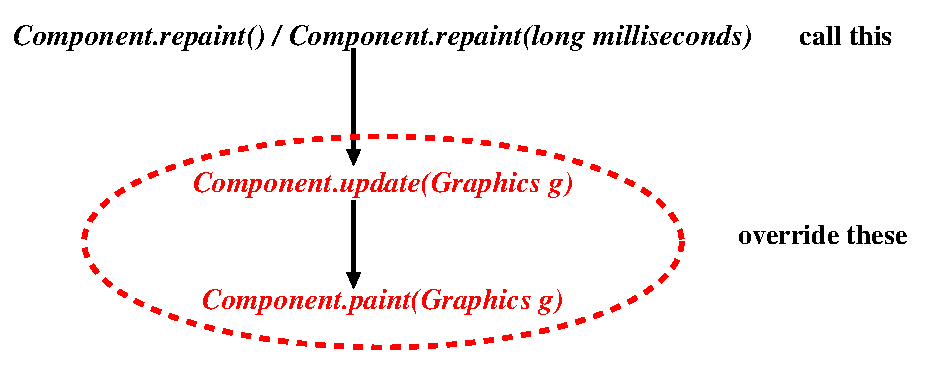
\includegraphics[width=\textwidth]{Figures/PaintMethod.eps}
    \caption{The default behaviour of the painting methods of components in the AWT package.}
    \label{fig:PaintMethod}
  \end{center}
\end{figure}

Having learned the basic graphical tools of the AWT with the help of
the most easy plot program, we can now apply what we have just learned
to the simulation of the radioactive decay.
\inputlisting{Listings_Java/RadioactiveDecay_easyplot.java}
Implementing the graphical facilities in the
\verb|RadioactiveDecay.java| code is easy. The output of 
the new program can be seen in figure \ref{fig:RDEasyPlot}.
\begin{figure}[htbp]
  \begin{center}
    \includegraphics[angle=-90,width=\textwidth]{Figures/RadioactiveDecayEasy.eps}
    \caption{The output of the easyplot version of the radioactive 
      decay program.}
    \label{fig:RDEasyPlot}
  \end{center}
\end{figure}

In the program code we immediately recognize
in the lines  56 to 81 the \verb|paint()| method. The results of the
simulation have to be scaled appropriately to fit in the Frame. The
curve is plotted with the method \verb|drawLine()|. Since we want to
plot also the exact analytical solution for the mean values in red we
set
\begin{verbatim}
  g.setcolor(Color.red)
\end{verbatim}
in line 74 before drawing the corresponding curve.

It is important to note that in the lines 21 to 24 
we have added the code
\begin{verbatim}
  frame.addWindowListener(...);
\end{verbatim}
which allows to handle the request to close the window. These ``events''
are in the \verb|java.awt.event| package and will be discussed later
in chapter \ref{sec:AWTAdvanced}. 

\subsection{Ptplot -- Extending Javas Graphics Capabilities}
The quality of the plot of the simulation results are rather poor
compared to high standards we are used to today. It is clear, that we
could now go on refining the plot with the help of the Java
AWT. Although this might be an interesting and instructive task, it is
not our primary interest in this book. Fortunately, there are advanced
2D graphics components which can be used in applets and
applications. One of these packages is Ptplot (you pronounce it
pee--tee--plot). The Ptplot package is released under the liberal UC
Berkley copyright. It has been developed by Edward A. Lee, C. Hylands,
and W. Wu. You are free to download it at
\href{http://ptolemy.eecs.berkeley.edu/java/ptolemy.plot2.0/ptolemy/plot}%
         {http://ptolemy.eecs.berkeley.edu/java/ptolemy.plot2.0/ptolemy/plot}
where you also find
the documentation and many demos of Ptplot. 

The components of Ptplot have the following properties:
\begin{itemize}
\item plots are embeddable in applets and applications
\item you may use binary or ASCII data
\item the plots are auto--ranging
\item you may label automatically or manually the axes
\item logarithmic axes
\item live, animated plots
\item infinite zooming
\item  various plot styles (connected lines, scatter plots, bars, ..)
\item various point styles (none, dots, points, ....)
\item multiple data sets and legends
\item color or black and white plots
\item error bars.
\end{itemize}
Before writing the first program using Ptplot take a look at the
class hierarchy of Ptplot in figure \ref{fig:PtplotHierarchy}.
\begin{figure}[htbp]
  \begin{center}
    \leavevmode
    \setlength{\unitlength}{.8cm}
    \input{Figures/PtplotHierarchy1.pic}\\[.3cm]
    \input{Figures/PtplotHierarchy2.pic}
    \caption{The class hierarchy of the Ptplot package.}
    \label{fig:PtplotHierarchy}
  \end{center}
\end{figure}

Let us now look at a very simple program in order to demonstrate
what you need to invoke the Ptplot methods.
\inputlisting{Listings_Java/Ptplot_Demo1.java}

We see that we have to import additionally the  Ptplot package. The
class \verb|ptplot_Demo| extends the class \verb|PlotApplet|. Again we
want to run the code as applet as well as an application so the class
does have a main method. In lines 14 to 17 we instantiate the new Frame
and activate the WindowListener as we did it in the
\verb|RadioactiveDecay_ploteasy.java| code. The actual plot routines
are in lines 28 to 33. In the \verb|init()| method we invoke the method
\verb|super.newPlot()| to create a new plot, \verb|super.init()| to
initialize it and \verb|plot().setTitle| to give the plot a title.

A second possibility of using Ptplot, which we prefer to use, is to extend
the \verb|Applet| class instead of the \verb|PlotApplet| class and 
change the lines 28 to 33 to:
\lstinputlisting[first=28,last=33]{Listings_Java/Ptplot_Demo2.java}
The difference is that the \verb|PlotApplet| class realizes a kind
of interface for an applet to start plot commands confirming to the
pxgraph commands and executes them from parameters given in the applet.
Pxgraph is a program for the X windows system to plot data using
batch files like gnuplot. The full pxgraph functionality is
included in the ptplot package and can be used. For further documentation
concerning this point, please refer to the ptplot documentation.

Next we want to draw the results of the simulation of the radioactive
decay process with the help of Ptplot and learn at the same time how
to exploit the features of Ptplot. The corresponding code can be seen
below.
\inputlisting{Listings_Java/RadioactiveDecay_ptplot.java}
The output of the code can be seen in Fig. (\ref{fig:ptplotOutput}). 
\begin{figure}[htbp]
  \begin{center}
    \leavevmode
    \includegraphics[angle=-90,width=\textwidth]{Figures/RadioactiveDecay_ptplot.eps}
    \caption{The output of the RadioactiveDecay\_ptplot.java program.}
    \label{fig:ptplotOutput}
  \end{center}
\end{figure}

The actual plotting code starts in line 55 and ends in line 79. 
There we use several methods of the \verb|ptplot.Plot|
class and of the superclass \verb|PlotBox| of the \verb|Plot| class.
All methods are called \verb|setMethod| where \verb|Method| is
self-explaining. Several other methods are implemented in the
\verb|Ptplot.PlotBox| class and its child, the \verb|Ptplot.Plot| class. 
They are summarized in table \ref{tab:PtplotMethods}. 
\begin{table}[htbp]
  \begin{center}
    \small
    \leavevmode
    \begin{tabular}{p{5cm}|p{8cm}}
      Method & Purpose \\\hline\hline
      \verb|addLegend(int, String)| & draw a legend for one plot number\\
      \verb|addXTick()| & \\
      \verb|addYTick()| & \\
      \verb|setBackground(Color)| & set the background color of plot\\
      \verb|setForeground(Color)| & set the foreground color of plot\\
      \verb|setGrid(boolean)| & draw a grid \\
      \verb|setLabelFont(String)| & font for axis labels and legend labels  \\
      \verb|setTitle(String)| & title of graph \\
      \verb|setTitleFont(String)| & set title font \\
      \verb|setXLabel(String)| & label of x axis \\
      \verb|setYLabel(String)| & label of y axis \\
      \verb|setXLog(boolean)| & x axis logarithmic scaling \\
      \verb|setYLog(boolean)| & y axis logarithmic scaling \\
      \verb|setXRange(double, double)| & x range of the plot \\
      \verb|setYRange(double, double)| & y range of the plot \\\hline
      \verb|addPoint(int, double, double, boolean)| & add a point to the plot,
      the boolean var. decides, if the point gets connected with the last one.
      The integer var. is the plot number.\\
      \verb|addPointWithErrorBars(int,| 
                     \verb|double, double, double, double, boolean)| & %
      add a point to the plot with errorbars. Th additional vars. specify the
      lower and higer y coordinate of the error bar.\\
      \verb|setBars(boolean)| & bar plotting on or off \\
      \verb|setBars(double, double)| & define width and offset for bar 
      plotting and enable bar plotting. \\
      \verb|setImpulses(boolean)| & plot impulses \\
      \verb|setMarksStyle(String)| & none, points or various \\
    \end{tabular}
    \caption{Overview of all the Ptplot methods in the Plot and PlotBox classes.}
    \label{tab:PtplotMethods}
  \end{center}
\end{table}

Although this is the most common way of using ptplot in this book, there
is another feature coming with ptplot. It can read data files and plot
the data. For this you have to write a script, which contains the
commands for the plot to be created. This scripting language
is borrowed from the \emph{pxgraph} program. It is like using ``gnuplot''
 with
its scripting facilities. For details you can look at the 
documentation coming with the ptplot package. For us it will be
easier to read the files into Java and then use ptplot to plot it on 
screen.

%%%%%%%%%%%%%%%%%%%%%%%%
\subsection{3D plots in Java -- Java3D}
Sometimes you are forced to use 3D plots to visualize your data
and therefore it is natural to ask for a package to accomplish
three dimensional plots. Unfortunately to our knowledge there is
(yet) no freely available package in Java for 3D plots. Ptplot
can only handle 2D plots and JSci can handle only some very
basic 3D plots (see chapter \ref{sec:JSci}).

There is also a program called 
\verb|SciVis|\footnote{\href{http://kopernik.npac.syr.edu:8888/scivis/}%
  {http://kopernik.npac.syr.edu:8888/scivis/}},
which is completely written in Java and allows for 2D and 3D plots
in many different ways. But up to now, there are only C and
Fortran interfaces to supply data to it. You can also read from
files, but first you have to understand the data format, which is
described in the users guide.
The authors told us they are developing a Java interface to
supply data directly to \verb|SciVis|. 

At the moment, the best solution is to write the data to a file
and use an external program available to you. The most common
denominator would possibly be ``gnuplot'', which is available for many
different platforms and can create a lot of different 3D plots.

Since Java 2, there is a new (external) API -- not included in the JDK 1.2
disribution, you have to get it seperatly -- called \emph{Java3D}. 
This is a full implementation of three dimensional routines to
produce all kinds of 3D scenes and objects and even move these scenes.
With this API it seems to be possible to write a fairly easy
3D plotting program in the near future. So this lack of features
in Java for the scientist should be gone soon. 

%%%%%%%%%%%%%%%%%%%%%%%%%%%%%
\subsection{Using (system dependent) external programs like gnuplot}
There is a last way of obtaining 3D plots ``in Java'': You can use
an external program like Gnuplot or any other command line tool and
call it from a Java program. This of course is not system independent
and is not recommended unless you are desperatly needing it.

In Java there is a class called \verb|Runtime| in the \verb|java.lang|
package, which consists of all kind of methods to change and
use the environement you are running your Java program in. This can be used
to start a subprocess of the running Java program. So starting an
external process from a Java program can be done in two steps:
\begin{itemize}
\item Get a \verb|Runtime| object of the running Java program.
\item Start a new process as a subprocess of the given \verb|Runtime| object.
  You have to use the \verb|exec(String)| instance method of the  \verb|Process|
  class for this. 
\end{itemize}
You can also read the standard output of the subprocess and use it in your 
Java program. To demonstarte how it actually works, we give two examples:
\begin{enumerate}
\item A Java program starts a Gnuplot program, which plots a sine curve.
  \inputlisting{Listings_Java/Gnuplot.java}
\item A Java program executes a ``ls -al'' command on a UNIX machine,
  which just gives the directory listing. For a Windows system you just
  use the ``dir'' command instead.
  \inputlisting{Listings_Java/DirectoryListing.java}
  This time we also wait for the execution of the process to finish and 
  then read the standard output and display it on the screen.
\end{enumerate}

%%%%%%%%%%%%%%%%%%%%%%%%%%%%
\subsection{Printing in Java and with Ptplot}
Now that we have learned how to make plots in Java, it is of great
importance to get a printed version of our graphics. For
this purpose Java has commands for initiating a print job and preparing
the output for the printer. Java always produces potscript output.
Because the procedure has changed
from Java 1.1 to Java 2, we only present the Java 1.1 version not
to confuse you. In Java 1.0 there have been no methods for 
printing in  Java, you would have to use screen capture programs
for example.

Because printing is of course system dependent, it is not as easy
as issuing a print command, but it is still managable. 
In Java printing is done basically in four steps:
\begin{enumerate}
\item Get a \verb|Toolkit| for the component you want to print. 
  Use method \verb|getToolkit()| in the \verb|java.awt.Component| class.
\item Get a \verb|PrintJob|. Use the 
  \verb|getPrintJob(Frame f, String printjobname, Properties printprops)|
  method in the \verb|java.awt.Toolkit| class.
\item Start ``printing'':
  \begin{enumerate}
  \item Get the graphics context for the component in question. Use the
    \verb|getGraphics()| method of the \verb|java.awt.PrintJob| class.
  \item Print the desired part of the component. If you want to print 
    everything contained by the component use the \verb|printAll()|
    method, otherwise use just the \verb|print()| method of the
    \verb|Component| class.
  \item Send the data to the printer or file by using the \verb|dispose()|
    method of the \verb|java.awt.Graphics| class.
  \end{enumerate}
\item Finish printing and close dialog box. Use \verb|end()| method of
  the \verb|java.awt.PrintJob| class.
\end{enumerate}
The program \verb|RadioactiveDecay_printing.java| demonstartes the use of
the printing capabilities of Java. 
\lstinputlisting[first=32,last=47]{Listings_Java/RadioactiveDecay_printing.java} 

Of course there are some drawbacks to talk about. First of all with
this code you always get the output in a size referring to your actual
picture on the screen, it does not use the full paper size. If you want
to use the whole page size available you have to scale the component
to be plotted to the full size and scale back after printing. This is
what we do in the convenience class we have written for easy printing
in the simulation package. 

So if you want to print a component scaled to the full size, you use
the \verb|PrintComponent.Dialog()| method in the simulation package.
It scales your component to the full size -- no matter if it should be
on a portrait or landscape page -- and sends the scaled picture to the
printer or a postscript file. After printing it scales back to the
size it had before. The whole code above could therefore be
substituted by the line
\begin{verbatim}
  import simulation.*;
  ....
  PrintComponent.Dialog(frame, plot, "Radioactive Decay");
\end{verbatim}
Because most of the time you need postscript (or EPS) files of the
created plots or graphics, this is the most common use of the
printing features for a scientist.

A second method of the \verb|simulation| class called \verb|DialogNoScaling()|
can be used to produce unscaled output of the component or container.
I thas the same syntax as the \verb|Dialog()| method before.

There is one caveat to mention: if you are going to insert the
produced postscript files into TeX/LaTeX, you will have to do
some editing on the postscript files. First of all you have to
add a bounding box line at the beginning of the postscript
file. You can do this by hand, put a line (for a portrait figure)
\begin{verbatim}
 %%BoundingBox:  0 0 595 840
\end{verbatim}
at the beginning of the postscript file (You can adapt the numbers
to the figure at hand and check the area by viewing it in 
ghostscript/ghostview.) or you can use a program to automatically
calculate and insert a bounding box command (like e.g. epstool,
gsview on Windows, etc.). The second change is to remove all the 
lines between \verb|%%BeginSetup| and \verb|%%EndSetup| except
a possible rotate line like \verb|90 rotate 0 -595 translate|.
This is necessary, because some strange effects appear in the
resulting \verb|.dvi| or \verb|.ps| file after "texing".

Another drawback might be the resolution of the postscript file.
This happens especially when printing GUI components and is not
present when plotting ptplot plots fortunately. Java kind of rasters
the screen display and because the screen resolution is much worse 
than the printer resolution this gives unpleasant results. It also
gives strange results if you scale a large GUI to a small A4 or Letter
format for printing, which could look very ugly or even miss some
of the displayed objects. But as already mentioned, most of the time
we only need plots in postscript files and this works great with
the code above.

In Java 2 there has been some small changes to the printing
interface. A new class has been introduced in Java2: \verb|java.awt.print|.
This class provides much more sophisticated methods and it is even
able of handling color models, which is very important for
color handling and printing. This is a big step ahead, but for the
details we refer to the API documentation, because it is also a
bit more difficult to understand.

Ptplot 2.1 printing facilities ????? (EPS)

\paragraph{Printing from an Applet}
Usually applets are not allowed to initiate printjobs, unless
a \verb|SecurityManager|, another important Java class, explicitly
allows for it. Most of the time the browser or appletviewer has
to initiate the printjob, allowed by the security manager. You can of
course always use the printing facilities of the browser and plot
the whole panel visible in the browser.


What you can do is, write a main method in the applet and start
it as an application. Do the plots  and print them from the
application. 

If you use a security manager and are allowed to print, you need a
frame for your applet, because the  \verb|getPrintJob()| command
only takes a frame and not an applet as first argument. So just
put a frame into the applet and then put the applet inside the frame.


%%%%%%%%%%%%%%%%%%%%%%%
\subsection{The Results of the Simulation}

The results of the simulation are plotted in Fig. (\ref{FIG_DECAYA}) and 
(\ref{FIG_DECAYB}).
\begin{figure}
\label{FIG_DECAYA}
\begin{center}
\includegraphics[angle=-90,width=8cm]{Figures/RadioactiveDecay_1.eps}\\
\includegraphics[angle=-90,width=8cm]{Figures/RadioactiveDecay_2.eps}
\end{center}
\caption{Two realizations of the stochastic process of the radioactive decay.
The first one with linear y axis scaling and the second one uses a logarithmic
y axis scaling. The blue lines are the exact solution and the red ones
are the simulations.
The parameters of the simulation were choosen to be $N_0 = 100; 
\quad p = \lambda \Delta t = 0.01 s^{-1}; \quad \Delta t = 1\text{s};
\quad t_{\text{end}} = 300\text{s}$}
\end{figure}
\begin{figure}
\label{FIG_DECAYB}
\begin{center}
\includegraphics[angle=-90,width=11cm,clip]{Figures/RadioactiveDecay_3.eps}\\
\end{center}
\caption{The same as figure \ref{FIG_DECAYA}, but with different parameters:
$N_0 = 1000; \quad p = \lambda \Delta t = 0.03 s^{-1}; 
\quad \Delta t = 1\text{s};  \quad t_{\text{end}} = 100\text{s}$}
\end{figure}
 It is 
immediately recognized that the simulation results fluctuate around 
the expected curve. This is of course not astonishing since the 
exact result holds for mean values. In order to achieve a better
agreement with the decay law it is necessary to run the simulation
several times and to take the average over the different 
realizations of the decay process. This can easily be achieved by 
a simple modification of the program \verb|RadioactiveDecay_ptplot.java|.
 We introduce an additional input variable, the number of realizations
\verb|nreal| and accordingly implement a loop over the different 
realizations. This can be best seen in the listing of the 
new program \verb|RadioactiveDecay_ptplot2.java|.
\lstinputlisting[first=61,last=63]%
          {Listings_Java/RadioactiveDecay_ptplot2.java}

At the end of the realizations loop
we have to perform the average. This is seen in lines 61 to 63.
(STRESS MORE THE IDEA OF REALIZATIONS!!!!; allgemeine Strategie erlaeutern.)

Note that in order to speed up the program we have modified slightly 
the algorithm  so that we can save a loop. ?????
The probability to observe one decay in time $\Delta t$ is
\begin{equation}
p = \beta \Delta t
\end{equation}
where $\beta = \lambda N$ and $\Delta t$ must be small enough so 
that $\beta \delta t \ll 1$. 
From the elementary rules of combinatorics we know that
the probability to observe $n$ decays in time $t=m\Delta t$ is therefore
given by
\begin{equation}
P = p^n(1-p)^{m-n} {m \choose n}.
\end{equation}
Inserting the definition of $p$ the above expression can be cast 
in the form
\begin{equation}
P = \left( \frac{\beta t}{m}\right)^n 
     \left( \frac{1 - \beta t}{m} \right)^{m-n}
      \frac{m!}{(m-n)! n!}.
\end{equation}
Performing the limit $\Delta t \longrightarrow 0$ (i.e. $m 
\longrightarrow \infty$) and considering that
\begin{equation}
\left(1-  \frac{\beta t}{m} \right)^{m} \longrightarrow 
            \exp(-\beta t),
\end{equation}
\begin{equation}
\left( 1- \frac{ \beta t}{m} \right)^{-n} \longrightarrow 
            1,
\end{equation}
and
\begin{equation}
\frac{m!}{(m-n)! n!} \longrightarrow m^n
\end{equation}
we obtain the result
\begin{equation}
P = \frac{\mu^n \exp(-\mu)}{n!},
\end{equation}
where $\mu = \beta t$. The above distribution is the well know
Poisson distribution.

\subsubsection{Plot Methods in the Simulation Package}
Because sometimes it is easier to use ready made routines, we
have added some plotting convenience classes and methods to
get the plots faster. If you take the shortcut presented here
or you want to use the low level ptplot interface does not 
matter, it is totally up to you.

?????
\paragraph{plot2D()}
\paragraph{errorBars()}
\paragraph{histogram()}
\paragraph{barPlots()}

It is now easy to verify that the number of decays in a given 
interval is distributed according to the Poisson distribution.
To this end we have counted the number of decays in a given 
interval. This is accomplished in the lines xy. At the end of the
program we plot in a histogram the distribution of the number of 
decays and overlay the expected Poisson
distribution.  

\subsubsection{Listing of the full Program}
\lstinputlisting{Listings_Java/RadioactiveDecay_ptplot2.java}


Run the program for the following two sets of parameters:
\begin{eqnarray*}
N_0= 100, p = 0.001 s^{-1}, \Delta t = 1s, t = 100s \\
N_0= 100, p = 0.0001 s^{-1}, \Delta t = 1s, t = 100s
\end{eqnarray*}
with nreal = 100 and nreal = 1000.

The result of  two simulations can be seen in figs. x and y.
\begin{figure}
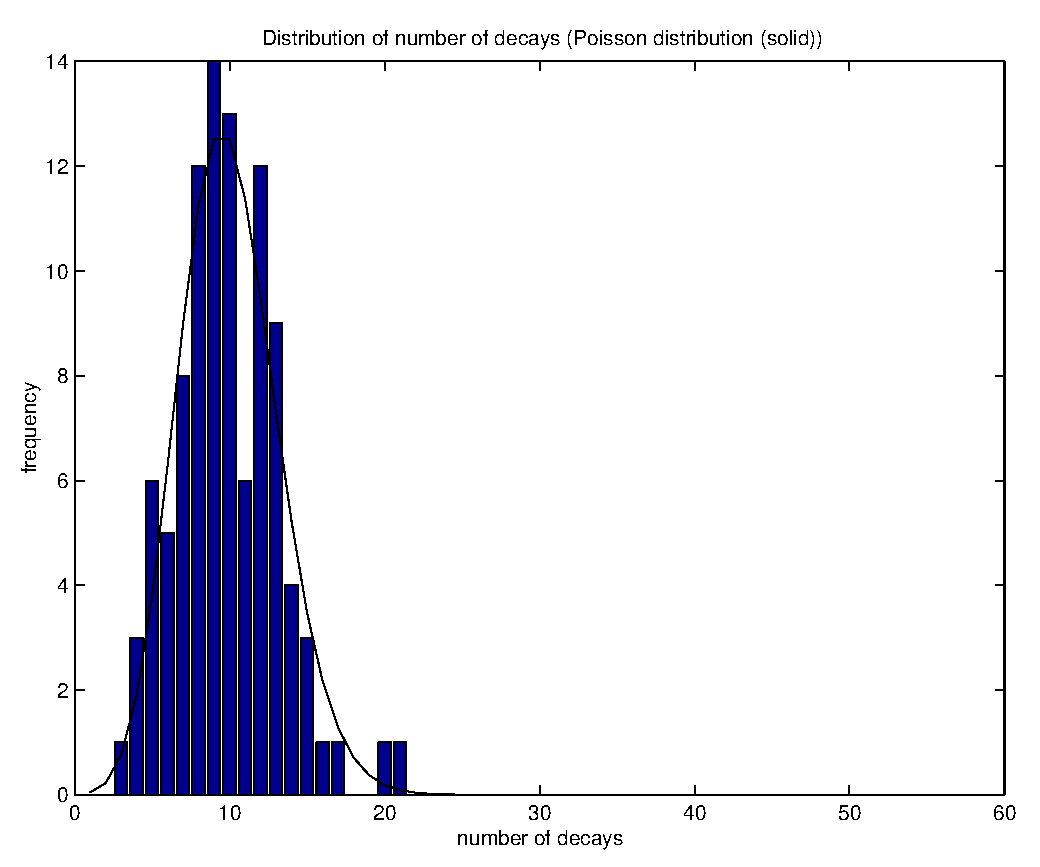
\includegraphics[width=\textwidth]{Figures/f_decay1.eps}
\caption{The distribution of the number of decays computed with 
the program decayr. 100 realizations. The simulation was run for
N0=100 and lambda=0.001.}
\end{figure}

\begin{figure}
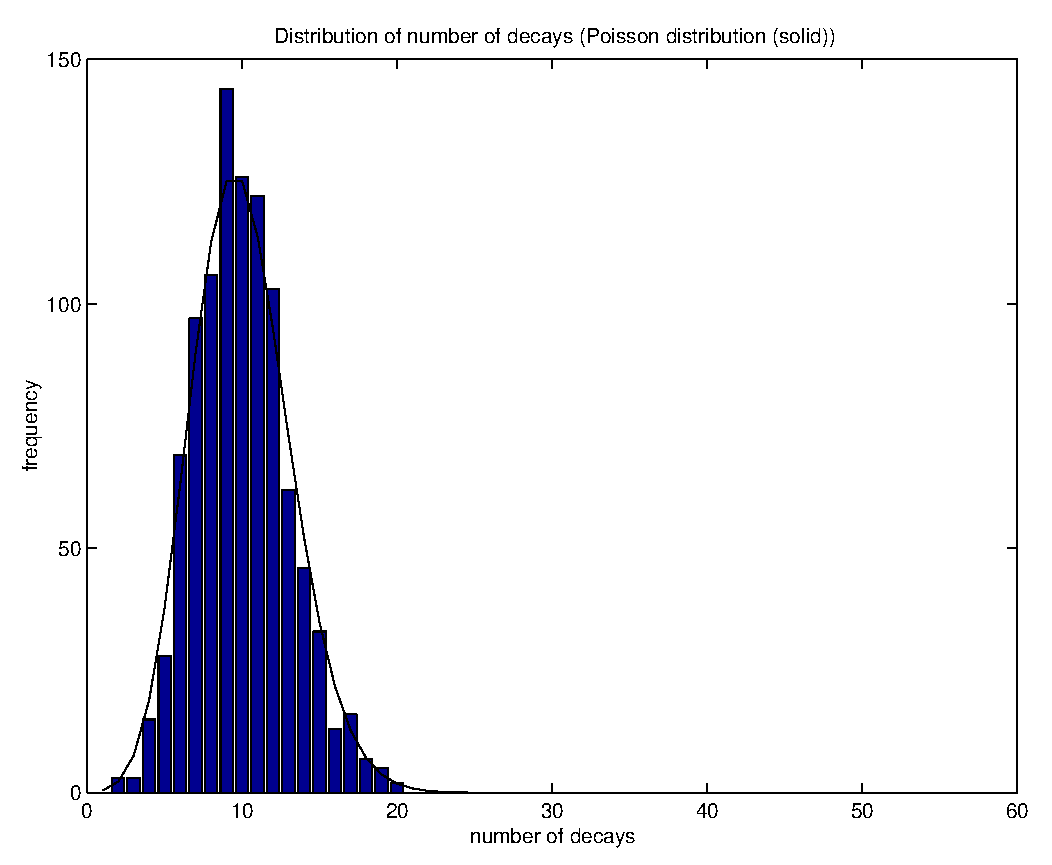
\includegraphics[width=\textwidth]{Figures/f_decay2.eps}
\caption{The distribution of the number of decays computed with 
the program decayr. 1000 realizations. The simulation was run
for N0=100 and lambda = 0.001.}
\end{figure}

%%%%%%%%%%%%%%%%%%%%%%%%%%%%%%%%%%%%%%%%%%%%%%%%%%%%%%%%%%%%%%%%%%%%%%
\section{Simple Monte Carlo Evaluation of Integrals}
It is the purpose of this subsection to introduce Monte Carlo Methods
in the context of the numerical evaluation of definite integrals.
We will see in later chapters that Monte Carlo integration is the
method of choice when treating multidimensional
integrals numerically. As a typical rule of thumb
``classical'' deterministic methods are outperformed
by Monte Carlo methods  for systems with a large number of 
degrees of freedom.
For simplicity and to stress the basic ideas 
it is convenient at the moment to consider one--dimensional definite
integrals of the form
\begin{equation}
\label{INTEGRAL}
I = \int_a^b dx f(x).
\end{equation}
Obviously such integrals can be evaluated analytically for many
integrands
$f(x)$.  However, there are as well many cases for which a numerical
evaluation is necessary.

Before introducing the Monte Carlo approach to numerical integration
let us remind the basic ``classical'' deterministic approach to
numerical integration. The standard approach is based upon the
geometrical interpretation of the integral (\ref{INTEGRAL}) as the
area under the curve of the function $f(x)$ between the points $a$ and
$b$. In the simplest algorithm this area (see figure) is approximated
as a sum over rectangles. To this end the $x$--axis is divided into
$n$ equally spaced intervals of width $\Delta x$,
\begin{equation}
\Delta x = \frac{b-a}{n}
\end{equation}
whose ends are given by
\begin{equation}
x_i = x_0 + i\Delta x
\end{equation}
for $i=1, \ldots ,n$. Of course, $x_0 = a$ and $x_n =b$. Thus in the
so--called rectangular approximation the integral is evaluated as
\begin{equation}
\label{I_CLASSICAL}
I_n = \Delta x \sum_{i=0}^{n-1} f(x_i).
\end{equation}
Of course, other more accurate approximations are possible.

How can we now evaluate the above integral by drawing random numbers?
The standard way is based on a very simple idea. 
From the introductory course in analysis we know that the Mean 
Value Theorem states that the exact value of the integral $I$ is 
given by
\begin{equation}
I= (b-a) f(\zeta)
\end{equation}
for some value of $\zeta$ in the interval $a \le \zeta \le b$. $f(\zeta)$
represents the average value of the function $f(x)$ 
in the interval $[a,b]$. Thus we could also write
\begin{equation}
I = (b-a) \langle f \rangle,
\end{equation}
where $\langle  \rangle$ denotes the mean value.
Let us draw $n$
random numbers which are uniformly distributed in the interval $[a,b]$
and let us sample the corresponding value of $f(x_i)=f_i$. The Monte Carlo
estimate $I_n$ of the integral $I$ is then the sample mean, which is
given by
\begin{equation}
\label{MCI_STANDARD}
I_n = \frac{(b-a)}{n} \sum_{i=1}^{n} f(x_i),
\end{equation}
where $n$ is the number of trials. Amazingly the form of the above
estimate is very similar to the classical formula (\ref{I_CLASSICAL}).
The fundamental difference is that now the $n$ points at which the
function $f$ is evaluated are no longer equally spaced but randomly 
distributed.

There is also the possibility to compute the integral $I$
stochastically
with the help of the ``Hit or Miss'' algorithm. The idea behind
this algorithm is again very simple. To be explicit we imagine a rectangle
of height $h$ and width $(b-a)$ such that the function $f(x)$ lies
within the rectangle (see figure; Gould, p.329). To evaluate the
integral we draw randomly pairs of uniformly distributed random
numbers $(x_i,y_i)$ such that $a \le x_i \le b$ and $0 \le y_i \le h$.
In other words the probability to draw a point within the rectangle is
given by the inverse of the area $A$ of the rectangle,
i.e. $1/(b-a)h$. It is now evident how the area under the
function $f$ may be estimated. The fraction of points $(x_i,y_i)$
which satisfy the condition $y_i \le f(x_i)$ is an estimate of the
ratio of the integral $I$ to the area $A$ of the rectangle. Hence,
drawing $n$ random pairs the estimate $I_n$ of $I$ by this ``scoring''
method is given by
\begin{equation}
I_n = A \frac{n_s}{n},
\end{equation}
where $n_s$ is the number of ``hits'', i.e., of points lying below the
curve $f(x)$.

Before writing two simple programs to elucidate the above algorithms
it is important to have in mind that both estimates are affected by
statistical errors. Let us consider for simplicity 
the standard method. Since the $f(x_i)$ are random we know 
from the elementary theory of data analysis
that an appropriate measure of the error is given by the variance
which is defined by
\begin{equation}
{\rm Var}(f) = \langle f^2 \rangle - \langle f \rangle^2.
= \langle (f -\langle f \rangle)^2 \rangle
\end{equation}
Since we draw a finite number of random numbers we can
estimate the mean value by using
\begin{equation}
\hat{f}  = \frac{1}{n} \sum_{i=1}^n f(x_i) 
\end{equation}
and correspondingly the estimate of the variance by using
\begin{equation}
{\rm Var}(f(x_1),\ldots, f(x_n)) = \frac{1}{n-1} \sum_{i=1}^n 
   (f(x_i)- \hat{f})^2 = \sigma_f^2.
\end{equation}
The quantity $\sigma_f = \sqrt{{\rm Var}(f_1, \ldots, f_n)}$ 
is also called the standard deviation. In the previous expression
we have used the short--hand
notation $f(x_i) = f_i$. However,
we are not interested in the error of $f$ but in the error of the
estimate $I_n$, which is a sum over random numbers. 

Repeating the 
simulation and hence drawing other random numbers we will get another
estimate of $I_n$. Therefore, repeating the simulation $m$ times 
we can estimate the mean of $I_n$ as
\begin{equation}
\hat{I_n} = \frac{1}{m} \sum_j^m I_n(j)
\end{equation}
and the corresponding variance as
\begin{equation}
{\rm Var}(I_n(1), \ldots, I_n(m)) = 
\frac{1}{m-1} \sum_j^m (I_n(j) - \hat{I_n})^2 = \sigma_I^2
\end{equation}
We will denote the above variance also by $\sigma_I^2$.
Of course, proceeding this way is not very practical since we
have to perform the simulation $m$ times. A much more economical
estimation of the error of the mean of $I_n$ could be achieved by 
establishing a simple relation between $\sigma_I$ and the standard 
deviation of the individual trials $\sigma_f$. To this end we 
introduce the discrepancy $\delta f_i$ between the
individual trial $f_i$ and its mean $\langle f \rangle$. The 
discrepancy $\delta I_n$ between $I_n$ and its mean value can be
obtained to first order in the $\delta f_i$ by a simple Taylor 
expansion (error propagation rules)
\begin{equation}
\delta I_n = \sum_{i=1}^n \frac{\partial I_n}{\partial f_i} \delta 
f_i.
\end{equation}
Hence, it follows from the above equation by taking the average over
$\delta I_n^2$ that
\begin{equation}
\langle \delta I_n^2 \rangle = \sum_{i,j=1}^{n}
    \frac{\partial^2 I_n}{\partial f_i \partial f_j} 
     \langle \delta f_i \delta f_j \rangle.
\end{equation}
It is plausible to assume, that 
$\langle \delta f_i \rangle = 0$
for all $i$ and that the $\delta f_i$ are not correlated
for $i \neq j$, i.e.,
$\langle \delta f_i \delta f_j \rangle = \langle f_i \rangle \langle f_j \rangle$
and that for $i=j$ we have $\langle \delta f_i^2 \rangle = \sigma_f$ 
for all $i$ it follows from the above equation that
\begin{equation}
\sigma_I^2 = \sum_{i=1}^n \left(
      \frac{\partial I_n}{\partial f_i} \right)^2 \sigma_f^2
      = \frac{1}{n^2} n \sigma_f^2 = \frac{\sigma_f^2}{n}
\end{equation}
and finally we have the useful relation
\begin{equation}
\sigma_I = \frac{\sigma_f}{\sqrt{n}}.
\end{equation}
The mean error of the mean scale with 1 over the square root of 
the number of individual trials. The precision of the estimate 
thus increases only slowly with the number of trials (remark: central
limit theorem: see Chapter 2).

Now we are in the position to write two programs to implement the above
stochastic algorithms. In order to be specific we compute the integral
\begin{equation}
I = \int_0^1 dx \sqrt{1-x^2} = \frac{\pi}{4}.
\end{equation}
In other words we want to estimate the number $\pi$ by Monte Carlo
methods.

We begin by the standard method. The listing of an according 
program can be seen below.

\subsubsection{Listing of the program mcpi.}
\inputlisting{./Listings/mcpi.m}

We run the program for $n=10, 100, 1000, 10000$. The result of the 
four simulations can be seen in Fig. xy.
\begin{figure}
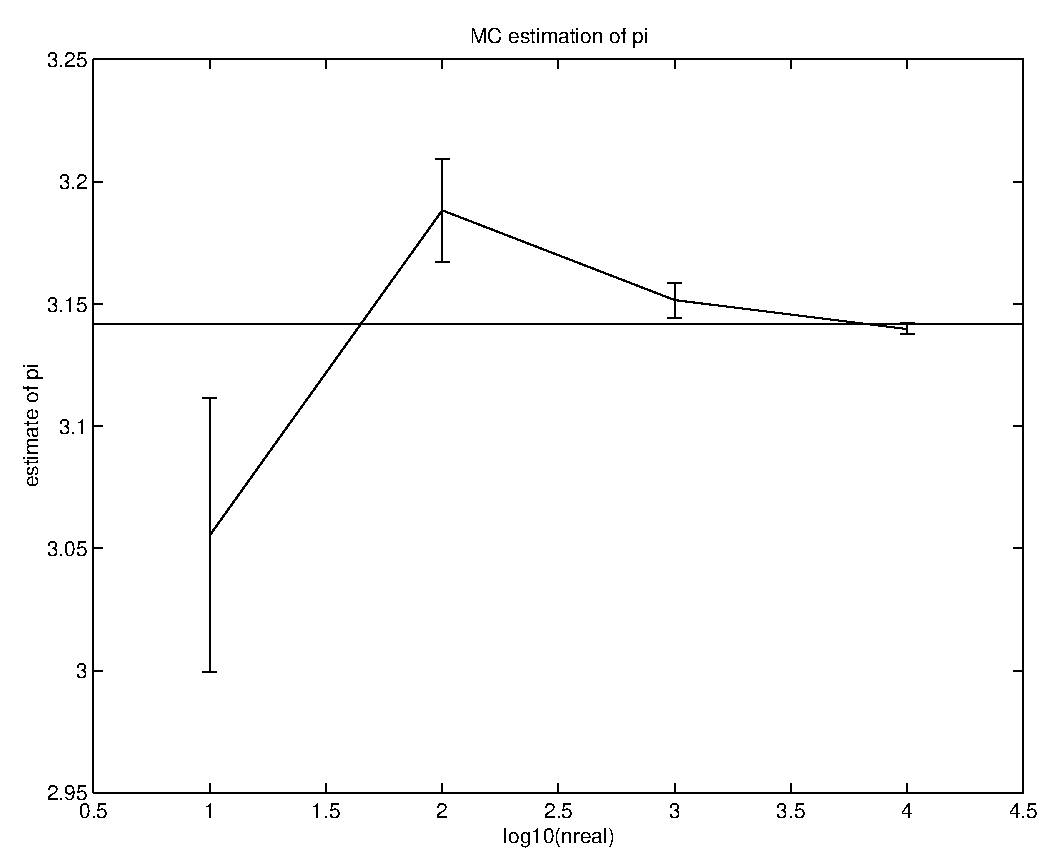
\includegraphics[width=\textwidth]{Figures/plotmcpi.eps}
\caption{The estimation of pi for n=10,100,1000,10000. The 
error bars correspond to the standard deviation of the mean of the 
estimate.}
\end{figure}

Next we write a program for the scoring  method. 

\subsubsection{Listing of the program mcpiscore.m}
\inputlisting{./Listings/mcpiscore.m}

Again we run the simulation for n=10, 100, 1000, 10000.
The result of a simulation can be seen in the next Figure.
\begin{figure}
\begin{center}
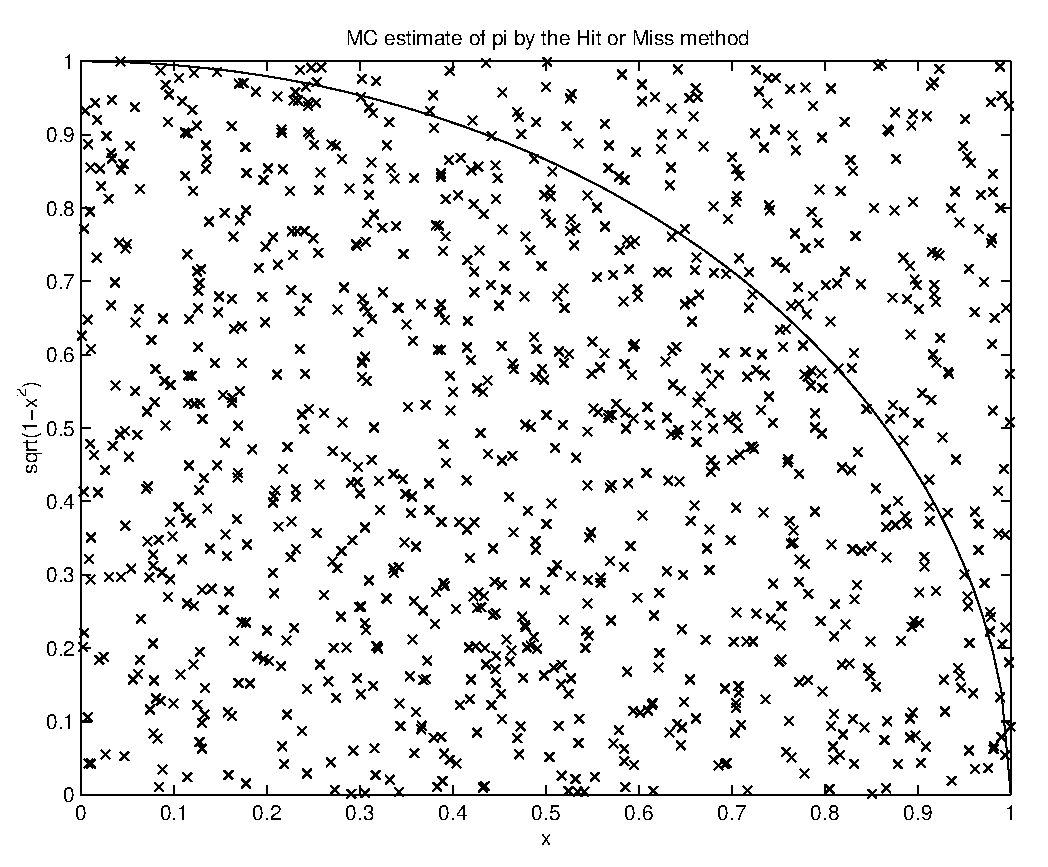
\includegraphics[width=.7\textwidth]{Figures/fmcpiscore.eps}
\end{center}
\caption{The scoring method. The continuous line represents
the function $\sqrt{(1-x^2)}$.}
\end{figure}


%%%%%%%%%%%%%%%%%%%%%%%%%%%%%%%%%%%%%%%%%%%%%%%%%%%%%%%%%%%%%%%%
\section{Beyond this chapter}


%%%%%%%%%%%%%%%%%%%%%%%%%%%%%%%%%%%%%%%%%%%%%%%%%%%%%%%%%%%%%%%%
\section{Exercises}

Use the  Matlab function \texttt{rand()}
to solve the following problems (don��t care about the quality and
the algorithm of the random number generator, for now):

\begin{Ex}
\label{Photoabsorption}
\textbf{Photoabsorption \cite[]{reif:67}} \\
Consider the absorption of photons passing through a gas in two dimensions.
We model the gas by introducing slabs of width $dx$ and density $n$ (in
particles per area), which absorb the incident photons. The slab
particles have a cross-sectional area of $\sigma$.

So the probability of a photon to be absorbed in the slab will be
($M$ is the number of particles in the slab of the height $dy$)
$$ P(\text{Photon absorbed}) = \frac{M\sigma}{dy} =
      \frac{\sigma n dx dy}{dy} = \sigma n dx  \quad .$$
We have assumed that there is no overlap between the cross-sections of
the slab particles.

Write a program to simulate this process on the computer. Take $N$
incident photons and watch the number of particles left over
against the slabs passed in a diagram. Do this simulation several
times and calculate the ensemble-average. What process you know
is similar to this behaviour and what takes the place of the spatial
dimension in that case?

%If we now have N identical slabs in a row, the probability of passing
%through all the slabs would be $(1-p)^N$, if the transmissions
%are statistically independent of each other.
%Then for a slab of finite thickness $X=N dx$ with $N\to\infty$, we
%get the Transmission probability
%$$ P(\text{transmitted through $N$ slabs}) =
%       \left(1-\frac{n\sigmaX}{N}\right)^N \quad .$$

%Now simulate the following systems:
%identical photons are absorbed in one slab ($N$ slabs)
\end{Ex}

\begin{Ex}
\label{Monte-Carlo_Integration}
\textbf{Monte-Carlo Integration -- Speed and Accuracy} \\
Write a program for the calculation of the following integral:
$$ \int_0^1 \frac{1}{1+x^2} dx\quad .$$
\begin{enumerate}
\item using the hit and miss method
\item using the standard method
\end{enumerate}
For both algorithms, calculate the mean and the standard deviation
as discussed in the lecture. Also use the analytical result of the
integral to calculate $\pi$. Compare the accuracy of both algorithms
using the approximations of $\pi$. Compare the speed of the two
programs by using the \texttt{cputime} function in Matlab.
(e.g. type the following to time the random number generator:
\texttt{t=cputime;x=rand(1000);cputime-t})

To that end, create a table and a plot with the two parameters
($n$: the number of intervals and $N$: the number of realizations)
against
the accuracy (use at least 5 values). To save time, you can first
check for a good $n$  and then do the plots only against $N$.
For the speed, plot the cputime against the achieved accuracy for
many different $N$.
\end{Ex}

\begin{Ex}
\label{Euler_Constant}
\textbf{Euler��s Constant using Monte-Carlo Algorithm %
          \cite[]{mohazzabi:98}} \\
Suppose throwing $N$ darts randomly at a dart board, which has been
divided into $R$ equal size regions. The probability of hitting one region
is $p=1/R$. Then the probability of hitting an empty region
(not already occupied by a dart) is $(1-p)^N$. Using the binomial
distribution, you can get the probability for hitting a region with
$m$ darts. If you choose
the number of regions equal to the number of darts
thrown on the board, we have $p=1/N$ and therefore
$$ P(\text{hitting an empty region}) = \left( 1-\frac{1}{N} \right)^N\quad .$$

Because the above series converges to $e$ for $N\to\infty$, we can use
the following method to get an approximation of the Euler constant:
\begin{enumerate}
\item[(i)] Throw randomly a large number of darts (say $N$) on a board, which has
  been divided into $N$ equal size regions.
\item[(ii)] Count the number of empty regions (call it $N_0$).
\item[(iii)] The fraction $N/N_0$ is a good estimate of the Euler constant $e$.
\end{enumerate}

Write a program for that algorithm and check the results. You can even
use $N/N_1$, if $N_1$ is the number of regions with the occupancy of
one dart. Check this, too. What $N$ do you need to
get the same accuracy using the formula? And how many terms of the
series for $e$ ($\sum_{i=0}^\infty 1/i! = e$)?
\end{Ex}

%%%%%%%%%%%%%%%%%%%%%%%%%%%%%%%


\bibliographystyle{peter}
\bibliography{V_98,simulit}

%%% Local Variables: 
%%% mode: latex
%%% TeX-master: "V_98"
%%% End: 


%%% Chapter 2 
%%%%%%
%%%%%% Chapter 2
%%%%%%

\chapter{Stochastic Variables}
Since the notion of random variables will be essential
for the understanding of stochastic methods this chapter will be 
devoted to the introduction of the fundamental concepts of 
probability theory.

%%%%%%%%%%%%%%%%%%%%%%%%%%%%%%%%%%%%%%%%%%%%%%%%%%%%%%%%%%%%%%%%%%
\section{The Nature of Probabilities}
In the previous chapter we have already made use of probabilistic 
notions in an intuitive way. However, we have not asked the 
following question: What are probabilities? How can we formulate 
the notion of probability in such a way that it is useful for 
physical applications?

Essentially, there are three possible definitions of probability
\cite{BRODY}:
a) the axiomatic interpretation, b) the frequency interpretation, and
c) the ensemble interpretation.


\subsection{The Axiomatic Interpretation}
The axiomatic definition \cite{FELLER} of probabilities has been proposed by 
Kolmogorov in 1933. The formal objects to which we want to 
attribute probabilities are called {\em events} and are subsets
of a basic set $\Omega$ which is called the {\em event space} or in 
physical applications the {\em phase space}. If the event $e$ 
belongs to $\Omega$, so does its complement $\Omega - e$ also; the 
null event $\oslash$ is therefore also in $\Omega$. Events 
containing only one member of $\Omega$ are called the elementary events
of $\Omega$.

A function $P(e)$, called the {\em probability} of $e$ can be 
assigned to each event $e$ in $\Omega$. The function $P(e)$ has
the following properties:

(i) $P(e) \ge 0$ for all $e$ in $\Omega$;

(ii) $P(\Omega) = 1$;

(iii) If $e_1, e_2, \ldots $ are in $\Omega$ and are pairwise
disjoint, i.e., $e_i \cap e_j = \oslash$ when $i \ne j$, then
$P(e_1 \cup e_2 \cup \ldots ) = P(e_1)+P(e_2) + \ldots$.

It follows immediately from the above three axioms that

(iv) If $\bar{e}$ is the complement of $e$, i.e., the set of all 
events which are not in $e$, then
$P(\bar{e}) = 1- P(e)$;

(v) $P(\oslash) = 0$.



\subsection{The Relative Frequency Interpretation}
In his attempt to axiomatize probability theory, von Mises
introduced in 1919 the notion of a {\em Kollektiv}, which stands
for a single infinite sequence of random events such as the 
outcomes of throwing a coin. He defined then the probability of some 
event to be the limit of its relative frequency in such a series of 
observations when the series becomes infinitely long (the 
Kollektiv) \cite{COMPAGNER,BRODY}. 
If we denote by $n$ the number of data in the series,
by $m(e)$ the number of times the event is observed in it, then
the probability $P(e)$ is defined as
\begin{equation}
P(e) = \lim_{n \rightarrow \infty} \frac{m(e)}{n}.
\end{equation}
Of course, such a series of events must have the property that any 
infinite subsequence in it must have the same limit. 

The problem with this definition is the following one: How can any 
sequence of experimental data, which will be always be finite, 
have the properties of such a Kollektiv? In practice the 
relative frequencies for subsequencies will always differ from 
that in the main sequence.

To illustrate the problems with the frequency interpretation of
probabilities we consider the following example. We throw a die 
$n$ times and
look at the relative frequency $m(4)$ of the outcome of throwing a 
4. This experiment will be simulated with the help of the 
following program.

{\bf Listing of the program relfreq.}
\inputlisting{./Listings/relfreq.m}

The result of an experiment for up to 400 throws is shown in Fig. 
(\ref{F_FRELFREQ}). Running the program again we observe 
another approach to the asymptotic
value. We recognize immediately the difficulties with von Mises 
definition of probability.
\begin{figure}
\label{F_FRELFREQ}
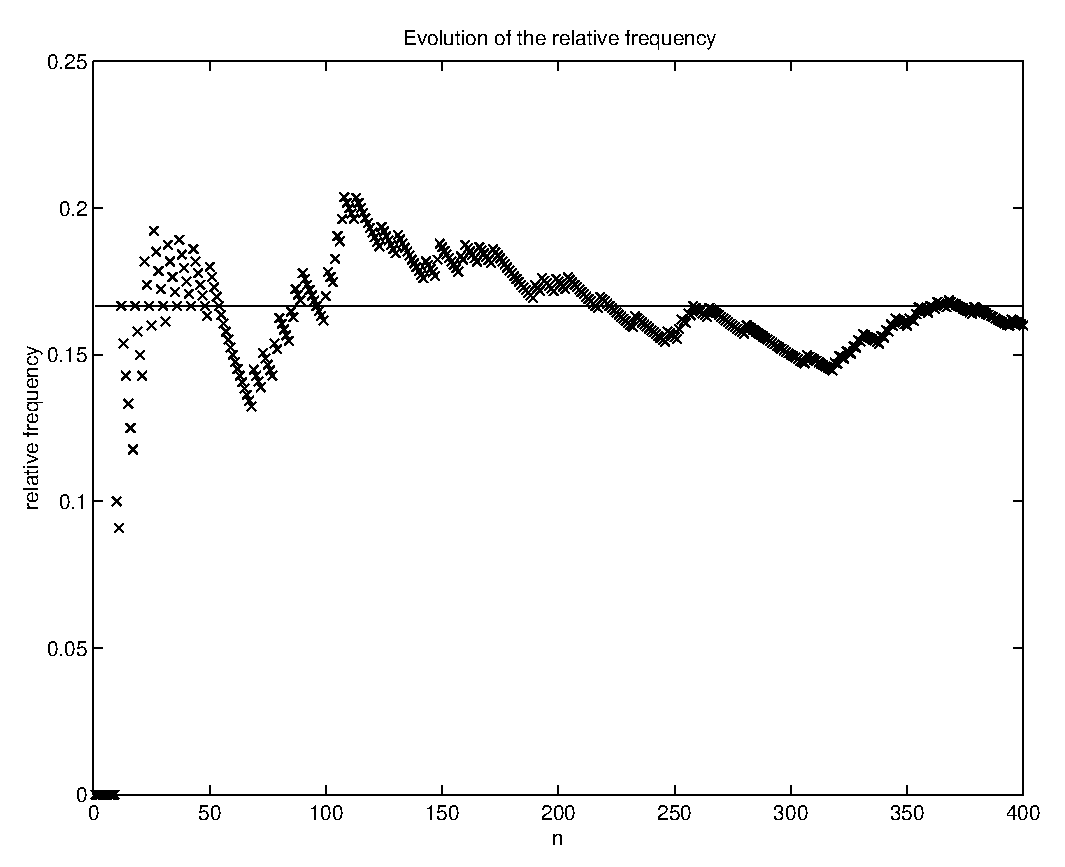
\includegraphics[width=10cm]{frelfreq.eps}
\caption{Simulation of the evolution of the relative frequency of throwing
a 4 in play of die.}
\end{figure}

\subsection{The Ensemble Interpretation}
We know from statistical mechanics  the notion of {\em ensemble}. An
ensemble is a collection of a large number $N$ of equally prepared
systems (equal models). A simple example is the microcanonical
ensemble, 
which is the
ensemble of all microstates in phase space, which are characterized by
fixing the macroscopic values for the the energy $E$, the volume $V$
and the number of particles $N$.

The abstract concept of an ensemble allows naturally the definition
of a mean value. We have to consider two cases:

(i) The ensemble contains a finite, discrete number of models: 
Let $n$ be the number of models and $Q(i)$ the interesting quantity in
model $i$. The ensemble mean value $\langle Q \rangle$ is then defined
as
\begin{equation}
\langle Q \rangle = \sum_{i=1}^n \frac{Q(i)}{n}.
\end{equation}

(ii) The models are characterized by some continuous parameter, i.e.,
the initial positions of molecules in a gas: If we name the continuous
parameter $\omega$, the phase space as $\Omega$ , and $n(w)$ a weight
function characterizing the ensemble, then
\begin{equation}
\langle Q \rangle = \frac{ \int_{\Omega} Q(\omega) dn(\omega)}
                         {\int_{\Omega} dn(\omega)}.
\end{equation}
Usually, the function $n(\omega)$ can be derived on the basis of the
theoretical model on which the ensemble relies upon. 

Let us consider as a simple example from equilibrium statistical 
mechanics a gas consisting of $N$ particles. The microstates of 
the system are the points $(q,p) = (\vec{r}_1, \vec{r}_2, \ldots, \vec{r}_N,
\vec{p}_1,\ldots, \vec{p}_N)$ in the 6--dimensional phase space.
The probability to find the microsystem at time $t_0$ in a volume 
element $dV=d^{3N}qd^{3N}p$ around $(q,p)$ is given by
\begin{equation}
dw(q,p) = \rho(q,p) d^{3N}qd^{3N}p,
\end{equation}
where $\rho(q,p)$ is the distribution function. For the 
microcanonical ensemble  the distribution function $\rho$ simply 
reads
\begin{equation}
\rho(q,p) = \left\{ 
\begin{array}{ll}
c= {\rm const}, &{\rm for} \quad E-\Delta \le H(q,p) \le E, \\
0, &{\rm otherwise}
\end{array} \right.
\end{equation}

Probabilities can be introduced as a special kind of ensemble 
average. Let $A$ be a property, which 
the members of the ensemble may have or not and let us define an indicator
function
\begin{equation}
\chi_A(\omega) = \left\{ 
\begin{array}{ll}
1, & {\rm if \quad member \quad labelled} \quad \omega {\rm \quad has 
\quad property\quad} A \\
0, & {rm if not}.
\end{array}\right.
\end{equation}
The probability of $A$ in the ensemble is  simply defined as 
the ensemble average of $\chi_A(\omega)$
\begin{equation}
P(A) = \langle \chi_A(\omega) \rangle = 
\frac{\int_{\Omega} \chi_A(\omega) dn(\omega)}{\int_{\Omega} 
dn(\omega)}.
\end{equation}
The probability is the relative weight in the ensemble of those 
members that have the property $A$. In the case of a discrete 
ensemble the above definition of probability reduces to a sum over
the members of the ensemble having the property $A$
\begin{equation}
P(A) = \sum_{i=1}^{n} \frac{\chi(i)}{n},
\end{equation}
i.e., the probability is the relative frequency of the members 
having the property $A$ in the ensemble.

It is clear that from the above definition of probability its is
possible to derive the Kolmogorov axioms of probability theory.

It is important to stress that the
ensemble is a purely theoretical construction and has to be adapted 
to the physical situation of interest as we will see in the future chapters. 
Furthermore, it is to be noted that the ensemble 
interpretation  allows the definition of time dependent 
probabilities,
i.e.,
\begin{equation}
P(A,t) = \langle \chi_A(t) \rangle,
\end{equation}
which are of fundamental importance while studying stochastic 
processes.

%%%%%%%%%%%%%%%%%%%%%%%%%%%%%%%%%%%%%%%%%%%%%%%%%%%%%%%%%%%%%%%%%%
\section{The Definition of Stochastic Variables}
A stochastic variable $X$ is an object which is defined by a space 
of states (space of events, phase space) and by a probability 
density over this set. The space of state may be discrete, e.g. 
the numbers 1,2,3,4,5,6 for a play of dice or the number of 
molecules in a chemical reaction, as well as continuous, e.g.
the velocity of a Brownian particle. Of course, the space of state
may also be discrete and continuous at the same time, e.g., the
energy of an electron in the presence of some binding centers.
When sampling a one dimensional continuous stochastic variable $X$,
the probability to find some value in the infinitesimal interval
$(x,x+dx)$ will be expressed symbolically by
\begin{equation}\label{DENSITYDEF}
P(x) dx \equiv {\rm Prob} \{X\in [x,x+dx] \},
\end{equation}
which defines the probability density $P(x)$ associated with the 
stochastic variable $X$. It follows immediately from the above 
equation and from the addition law of
probability theory that the probability to sample a value of $X$
in the interval $[a,b]$ is given by
\begin{equation}\label{DENSITYDEF2}
\int_a^b dx P(x) = {\rm Prob}\{ X \in[a,b] \}.
\end{equation}
It is evident from Eqs. (\ref{DENSITYDEF}) and (\ref{DENSITYDEF2}) that 
the probaility density is non--negative, i.e. $P(x) \ge 0$ and 
that it is normalized
\begin{equation}
\int_{-\infty}^{\infty} dx P(x) = 1.
\end{equation}
For later convenience we remark that the probability density may 
contain also sums over $\delta$--functions. For example $P(x)$ can 
also have the form 
\begin{equation}
P(x) = \sum_n p_n \delta(x-x_n) + \tilde{P}(x),
\end{equation}
where
$\tilde{P}(x) \ge 0$, $p_n \ge 0$, $\tilde{P}$ integrable  
and the normalization condition is
\begin{equation}
\sum_n p_n + \int dx \tilde{P}(x) =1.
\end{equation}

The distribution function $F$ of the stochastic variable $X$ is 
defined by 
\begin{equation}
F(x) \equiv {\rm Prob}\{X \le x\}.
\end{equation}
The density function and the distribution function are related by 
the equation
\begin{equation}
F(x) = \int_{-\infty}^x dx' P(x'),
\end{equation}
or equivalently by $F'(x)= P(x)$.

\subsection{Further Characterization of Stochastic Variables}
A stochastic variable is completely defined by the space of states 
and by the probability density function. However, it is helpful to 
introduce some other quantities in order to characterize them.

The {\em expectation value}, i.e. the average,  of any function $f(X)$ 
with respect to the stochastic variable $X$ is denoted by
$\langle f(X) \rangle$ and is defined by
\begin{equation}
\langle f(X) \rangle = \int dx f(x) P(x).
\end{equation}
Of particular importance are the {\em moments} of a distribution. The 
$m$--th moment $\mu_m$ is defined as $\langle X^m \rangle$. Of 
course, $\mu_1$ is the {\em mean}. The variance ${\rm Var}(X)$ 
is defined as
\begin{equation}
{\rm Var}(X) \equiv \langle (X - \langle X \rangle )^2\rangle
   = \mu_2 - \mu_1^2,
\end{equation}
and is the square of the standard deviation $\sigma$.

Another important quantity is the {\em characteristic function} $G(k)$. It is 
defined as
\begin{equation}
G(k) = \langle \exp(ikx) \rangle = \int_I \exp(ikx) P(x) dx,
\end{equation}
and has the obvious properties
\begin{equation}
G(0) = 1 \quad {\rm and} \quad |G(k)| \le 1.
\end{equation}
The characteristic function is also called the {\em the moment 
generating function}, because expanding the exponential function 
in a Taylor series we get 
\begin{equation}
G(k) = \sum_{n=0}^{\infty} \frac{i^n}{n!} k^n 
      \langle X^n \rangle.
\end{equation}
Thus, if $G(k)$ is known the moments are easily evaluated as
\begin{equation}
\left. \frac{d^n}{dk^n}G(k) \right| = i^n \langle X^n \rangle.
\end{equation}
The same function serves to generate the so--called cumulants
which are defined as
\begin{equation}
\ln G(k) = \sum_{n=1}^{\infty} \frac{(ik)^n}{n!} \kappa_n,
\end{equation}
and are combinations of the moments, i.e., the first three 
cumulants are given by
\begin{eqnarray}
\kappa_1 &=& \mu_1, \\
\kappa_2 &=& \mu_2 - \mu_1^2 =\sigma^2, \\
\kappa_3 & = & \mu_3 - 3 \mu_2 \mu_1 + 2 \mu_1^3.
\end{eqnarray}
It can be shown \cite{Gardiner} that the cumulant generating 
function  cannot be a polynomial of degree greater than 2, that 
is, either all but the first two cumulants vanish or there is an 
infinite number of nonvanishing cumulants.

REMARK ( kappai given then g(k) unique !!!???????????�) 

\subsection{Some Important Random Variables}
Let us first introduce and discuss briefly some important 
continuous one dimensional probability densities.

\subsubsection{The Uniform Density}
The simplest density is the uniform density which is constant if $x$
lies within the interval $[a,b]$ and zero otherwise, i.e.,
\begin{equation}
P(x) = 1/(b-a).
\end{equation}
It is easy to check that the mean of the uniform distribution is
\begin{equation}
\langle X \rangle = \frac{a+b}{2}
\end{equation}
and that the standard deviation of a uniformly distributed random variable 
is
\begin{equation}
\sigma = \frac{b-a}{2\sqrt{3}}.
\end{equation}
As we will see the uniform probability density will play a 
fundamental role in the forthcoming chapters.

\subsubsection{The Exponential Density Function} 
The exponential density function is defined as
\begin{equation}
P(x) = a \exp(-ax),
\end{equation}
where $a$ is any positive constant. It is easy to verify that
the mean and the standard deviation of an exponentially distributed random 
variable are equal
\begin{equation}
\langle X \rangle = \sigma = \frac{1}{a}.
\end{equation}

\subsubsection{The Gaussian or Normal Density Function}
The most important density function for physics is the 
gaussian probability density. It has the form
\begin{equation}
P(x) = (2\pi a^2)^{-1/2} \exp[-(x-x_0)^2/2a^2],
\end{equation}
for $a$ positive and $-\infty < x_0 < \infty$.
The mean and the standard deviation of the Gaussian probability 
density are given by $\mu_1 = x_0$ and by $\sigma =a$, 
respectively. The characteristic function of the Gaussian density reads
\begin{equation}
G(k) = \exp(i \mu_1k - \frac{1}{2} \sigma^2 k^2),
\end{equation} 
which means that $\kappa_1 = \mu_1$, $\kappa_2 = \sigma^2$ and 
that all higher cumulants vanish.

\subsubsection{The Cauchy or Lorentz Density} 
The Cauchy or Lorentz density is defined as
\begin{equation}
P(x) = \frac{1}{\pi} \frac{a}{(x-x_0)^2 + a^2}
\end{equation}
for positive $a$ and $-\infty <x_0 < \infty$. It is an example of 
a probability density which does not have a finite variance. In 
fact, not even the integral defining  the mean value converges. 

Let us now discuss some typical discrete probability densities.
The discrete random variable will be denoted by $N$.

\subsubsection{The Discrete Uniform Probability Density} 
The discrete uniform probability density is defined by
\begin{equation}
P(n) = \frac{1}{n_2 -n_1 +1}
\end{equation}
for $n_1 \le n \le n_2$ and zero otherwise. Of course,
$n_1$ and $n_2$ are integer numbers and $n_1 \le n_2$.
Its mean value is
\begin{equation}
\langle N \rangle = \sum_n n P(n) = \frac{n_1 +n_2}{2} 
\end{equation}
and its variance
\begin{equation}
\sigma^2 = \frac{(n_2 -n_1)(n_2 -n_1+2)}{12}.
\end{equation}
The above equations are easily proven with the help of the 
relations
\begin{equation}
\sum_{n=1}^N n= \frac{N(N+1)}{2}; \sum_{n=1}^{N} n^2 = \frac{N(N+1)(2N+1)}{6}. 
\end{equation}

\subsubsection{The Binomial Distribution}
Let us assume that the random variable $Y$ 
can take only two values $\{y_1,y_2\}$, the probability for the 
value $y_1$ being $p$ and correspondingly for $y_2$ (1-p). If we 
consider $N$ realizations of the stochastic variable $Y$ the 
probability to find the value $y_1$ $N$ times under the $n$ results
is the binomial density $P(n)$
\begin{equation}
P(n) = \frac{N!}{n!(N-n)!} p^n(1-p)^{(N-n)},
\end{equation}
for $0 \le n \le N$.
The mean and variance of the binomial density are given by
\begin{equation}
\langle n \rangle = Np,
\end{equation}
and
\begin{equation}
\sigma^2 = Np(1-p).
\end{equation}
It is easy to check the normalization of the binomial distribution since
\begin{equation}
1 = [p + (1-p)]^n = \sum_{n=0}^N \frac{N!}{n! (N-n)!}
        p^n (1-p)^{(N-n)}.
\end{equation}

\subsubsection{The Poisson Density}
The Poisson density as we already know
is defined as
\begin{equation}
P(n) = \frac{\exp(-a) a^n}{n!},
\end{equation}
for $n > 0$ and $a \in R$. The mean value and the variance
of the Poisson density are equal,
\begin{equation}
\langle n \rangle = \sigma^2 = a.
\end{equation}
As we already know from the discussion of the radioactive decay the 
Poisson density is a limit of the 
binomial probability density for $N \rightarrow \infty$, $p \rightarrow 
0$ while $Np=a={\rm const}$. Another limit of the Poisson density
which deserves consideration is the limit $a \gg 1$: In this limit
the Poisson density will be essentially different from zero only 
for $n \approx a$. For $n \gg 1$  the Stirling formula 
holds
\begin{equation}
n! \approx (2 \pi n)^{1/2} n^n \exp(-n)
\end{equation}
so we can write
\begin{equation}
\ln\left[ \frac{\exp(-a) a^n}{n!} (2\pi a)^{1/2} \right] 
\approx (n-a) -n\ln\left(\frac{n}{a}\right).
\end{equation}
Setting $\epsilon=(n-a)/2$ and since, 
for $\epsilon \ll 1$ $\ln(1+\epsilon) \approx \epsilon -
\epsilon^2/2$ and for $n\approx a$
we can write
\begin{equation}
\ln\left[ \frac{\exp(-a) a^n}{n!} (2\pi a)^{1/2} \right] \approx
-(n-a)^2\frac{1}{2a}.
\end{equation}
So that finally for $a \gg 1$
\begin{equation}
\frac{\exp(-a) a^n}{n!} \approx \exp\left( - 
\frac{(n-a)^2}{2a}\right).
\end{equation}
Thus, in the limit $a \gg 1$ the Poisson density resembles a
Gaussian density with mean $a$ and variance $a$.

\subsection{Multivariate Random Variables}
Up to now we have considered only one dimensional stochastic 
variables. Obviously, $n$ random variables $X_1, X_2, \ldots, X_n$ 
which are sampled simultaneously can be interpreted as the 
components of an $n$--dimensional stochastic variable $X$.
Their joint density function
$P_n(x_1, \ldots, x_n)$ is defined through the statement
\begin{equation}
P_n(x_1, \ldots, x_n)dx_1 dx_2 \ldots dx_n \equiv
{\rm Prob}\{ X_i \in (x_i,x_i+dx_i) \quad \text{for 
each} \quad i=1, \ldots , n\}.
\end{equation}
If we look at the subset of stochastic variables $X_1, \ldots 
X_s$, for $s>n$ we can easily write down with the help of the
elementary laws of probability theory the joint density function for 
this set irrespective of $X_{s+1}, \ldots, X_n$
\begin{equation}
P_s(x_1, \ldots, x_s) = \int P_n(x_1, \ldots, x_s, x_{s+1}, \ldots 
x_n) dx_{s+1} \ldots dx_{n}.
\end{equation}
$P_s$ is a so--called {\em marginal distribution}.

The {\em conditional density} 
$P_{s|n-s}(x_1,\dots,x_s|x_{s+1},\ldots,x_n)$ is the joint 
density of $X_1, \ldots , X_s$
given that $X_{s+1}=x_{s+1}$, \ldots , $X_n = x_n$ and is easily 
shown to be given by Bayes rule
\begin{equation}
P_{s|n-s}(x_1,\dots,x_s|x_{s+1},\ldots,x_n) =
\frac{P_n(x_1, \ldots, x_n)}{P_{n-s}(x_{s+1}, \ldots, x_n)}.
\end{equation}

Two subsets $(X_1, \ldots, X_s)$ and $(X_{s+1}, \ldots, X_n)$ are 
said to be statistically  independent if $P_n$ factorizes
\begin{equation}
P_n(x_1, \ldots, x_n)=P_s(x_1, \ldots, x_s)P_{n-s}(x_{s+1}, \ldots, 
x_n).
\end{equation}
In this case $P_s$ is the marginal as well as the conditional 
probability density.

The definition of moments is easily generalized to the  
multivariate case
\begin{equation}
\langle X_1^{m_1} \ldots X_n^{m_n} \rangle =
\int x_1^{m_1} \ldots x_n^{m_n} P(x_1, \ldots, x_n) dx_1 \ldots 
dx_n.
\end{equation}
Accordingly, the characteristic function is given by
\begin{equation}
G(k_1, \dots, k_n) = \left\langle 
\exp[i(k_1X_1 + \ldots +k_n X_n)]\right\rangle.
\end{equation}
Again the multivariate Taylor expansion in the variables $k_i$ 
generates the moments
\begin{equation}
G(k_1, \dots, k_n) = \sum \frac{(ik_1)^{m_1} \ldots (ik_n)^{m_n}}
                  {m_1! \ldots m_n!} 
       \langle X_1^{m_1} \ldots X_n^{m_n} \rangle.
\end{equation}
For completness we mention that the cumulants 
$\kappa(X_1^{m_1} \ldots X_n^{m_n})$ are defined as
\begin{equation}
\log G(k_1, \dots, k_n) = {\sum}' \frac{(ik_1)^{m_1} \ldots (ik_n)^{m_n}}
                  {m_1! \ldots m_n!} 
       \kappa(X_1^{m_1} \ldots X_n^{m_n}),
\end{equation}
where the symbol $\sum'$ idicates that we do not have to sum when 
all $m$ vanish. As an example we give the $n \times n$ covariance
matrix $\kappa(X_i X_j)$
\begin{eqnarray}
{\rm Cov}(X_i, X_j) &=& 
 \langle (X_i-\langle X_i \rangle)(X_j-\langle X_j \rangle)\rangle 
 \\
 & = & \langle X_i X_j \rangle - \langle X_i \rangle \langle X_j 
           \rangle.
 \end{eqnarray}
The diagonal elements of the covariance matrix are, of course, the 
variances, whereas the off--diagonal elements are called the 
covariances.
With the help of the covariance matrix it is possible to define a 
correlation coefficient
\begin{equation}
\rho_{ij} = \frac{\kappa(X_i X_j)}{\sqrt{\kappa(X_i^2) 
\kappa(X_j^2)}}.
\end{equation}
For $n=2$ the statistical independence of $X_1$ and $X_2$ can be 
expressed through one of the following criteria: 

(i) All moments 
factorize, i.e., $\langle X_1^{m_1} X_2^{m_2}\rangle= 
\langle X_1^{m_1}\rangle \langle X_2^{m_2}\rangle$. 

(ii) The 
characteristic function factorizes, i.e., $G(k_1,k_2) = 
G(k_1)G(k_2)$. 

(iii) All cumulants $\kappa(X_1^{m_1}X_2^{m_2})$ 
vanish when both $m_1$ and $m_2$ differ from zero. Two variables $X_1$
and $X_2$ are called uncorrelated if their covariance is zero. 
This condition is weaker than statistical independence.

A typical example of a multivariate density is the density of the multivariate 
Gaussian distribution
\begin{equation}
\label{MULTI_GAUSS}
p(\vec{x}) = \frac{(2\pi)^{-n/2}}{(\det A)^{1/2}}
     \exp\left( -\frac{1}{2} (\vec{x} - \vec{\mu})_i (A^{-1})_{ij} 
     (\vec{x}-\vec{\mu})_j \right),
\end{equation}
where $A$ is a symmetric, positive definite matrix with elements 
$A_{ij}$. It is straightforward to check that the mean value of $\vec{X}$
is given by
\begin{equation}
\langle \vec{X} \rangle = \vec{\mu},
\end{equation}
that the covariance matrix is given by
\begin{equation}
{\rm Cov}(X_i, X_j) = A_{ij},
\end{equation}
and that the generating function is
\begin{equation}
G(\vec{k}) = \exp(-\frac{1}{2} k_i A_{ij} k_j + i \mu_ik_i).
\end{equation}

%%%%%%%%%%%%%%%%%%%%%%%%%%%%%%%%%%%%%%%%%%%%%%%%%%%%%%%%%%%%%%%%%%
\section{The Random Variables Transformation Theorem}
We will discuss in this subsection a very helpful theorem by 
Gillespie. The proof of the theorem can be found in the book by
Gillespie \cite{GILLESPIE} or in his paper \cite{GILLESPIE_THEOREM}. 

We know already that a stochastic variable is defined by 
specifying its space of states and its probability density.
Here, we consider the $n$--dimensional random variables $X=(X_1, \ldots, X_n)$ 
which are specified by their joint probability density function
$P(x_1, \ldots, x_n)$. Let $f_i$ be functions of the $n$ variables. With the 
help of the $f_i$ we map the $n$ random variables $X_1, \ldots, X_n$ 
onto $m$  new random variables $Y_1, \ldots, Y_m$ by
\begin{equation}
Y_i = f_i(X).
\end{equation}
The random variable transformation theorem now states that the 
probability density of the new stochastic variable $Y$ is given by
the expression
\begin{eqnarray}
\label{RVT}
P(Y_1, \ldots, Y_m) &=& \int dx_1 \ldots dx_n \prod_{i=1}^{m} 
\delta(y_i - f_i(x_1, \ldots, x_n)) P(x_1, \ldots, x_n).
\end{eqnarray}
The integrals extend over the range of all $X_i$.
For a proof of the random variable transformation theory see 
Gillespie.

\subsection{The Addition of Stochastic Variables}
As a first simple example of the application of the random 
variable theorem we consider the addition of two stochastic 
variables $X_1$ and $X_2$ with joint probability density
$P(x_1,x_2)$. The probability density $P(Y) $ of a new stochastic variable
$Y$ which is defined as the sum of $X_1$ and $X_2$ 
\begin{equation}
Y = X_1 + X_2
\end{equation}
is then given by
\begin{equation}
P(y) = \int \int \delta(x_1 +x_2 -y) P(x_1,x_2) dx_1 dx_2.
\end{equation}
We can perform the integration over $x_1$ to obtain
\begin{equation}
P(y) = \int P(x_1,y-x_1) dx_1.
\end{equation}

For the special case of two statistically independent random 
variables $X_1$ and $X_2$ the above equation simplifies to the 
following expression
\begin{equation}
P(y) = \int P_{X_1}(x_1)P_{X_2}(y-x_1) dx_1.
\end{equation}

It is now easy to check that the following equations hold
for the mean value and for the variance of the new stochastic 
variable $Y=X_1 + X_2$
\begin{equation}
\mu(X_1 +X_2) = \mu(X_1) + \mu(X_2)
\end{equation}
and
\begin{equation*}
{\rm Var}(X_1 + X_2) = {\rm Var}(X_1) + {\rm Var}(X_2) +
            2 {\rm Cov}(X_1,X_2).
\end{equation*}
The last equation implies that only for uncorrelated stochastic 
variables we have the simple relation 
${\rm Var}(X_1 + X_2) = {\rm Var}(X_1) + {\rm Var}(X_2)$.

The above results for the mean values and variances can easily be 
generalized to the so called linear combination theorem. For any
set of random variables $X_1, \ldots, X_n$ and any set of 
constants $a_1,\ldots, a_n$ we have
\begin{equation*}
\mu\left\{  \sum_{i=1}^n a_i X_i \right\} =
     \sum_{i=1}^n a_i \mu(X_i) 
\end{equation*}
and
\begin{equation*}
{\rm Var}\left\{  \sum_{i=1}^n a_i X_i \right\} = 
    \sum_{i=1}^n a_i^2 {\rm Var}(X_i) + 
    2 \sum_{i=1}^{n-1} \sum_{j=i+1}^n a_i a_j {\rm Cov}(X_i,X_j).
\end{equation*}



\subsection{One--to--One Transformations}
Let us consider the following application of the random variables
transformation theorem. Let $X$ be a random variable with
probability density $P(x)$ and let the random variable $Y$ be 
defined as $Y=f(X)$. Then the density function of $Y$ is given by
\begin{equation}\label{ONE_TO_ONE}
P(y) = \int_{-\infty}^{\infty} dx P(x) \delta(y-f(x)).
\end{equation}
For the case that the function $f$ is a smooth, one--to--one
transformation the equation $y=f(x)$ can be solved uniquely for $x$
as $x=f^{-1}(y)$. Let us now change the integration variable in 
Eq. (\ref{ONE_TO_ONE}) from $x$ to $z=f(x)$
\begin{equation*}
P(y) = \int_{-\infty}^{\infty} dz \left| {f^{-1}}'(z) \right|
      P(f^{-1}(z)) \delta(y-z),
\end{equation*}
where we have made use of
\begin{equation*}
dx = \left|{f^{-1}}'(z) \right| dz.
\end{equation*}
Integrating over $z$ yields
\begin{equation*}
P(y) = P(f^{-1}(y)) \left|{f^{-1}}'(y) \right|.
\end{equation*}
Since $x=f^{-1}(y)$, then $|dx/dy|=|{f^{-1}}'(y))|$, and we can 
rewrite the above equation as
\begin{equation*}
P(y) = P(x) \left|  \frac{dx}{dy} \right|
\end{equation*}
which is a very important formula in the theory of stochastic 
variables which we will use, e.g., in the next chapter.

The previous result is easily generalized to many dimensions.
If the transformations $Y_i =f_i(X_1, \ldots, X_n)$ for $i=1,\ldots,n$ are 
one--to--one, then the probability density of the variables $Y_i$ 
is given by
\begin{equation*}
P(y_1, \ldots, y_n) = P(x_1, \ldots, x_n) 
     \left|  \frac{\partial(x_1, \ldots, x_n)}
     {\partial(y_1, \ldots, y_n)} \right|.
\end{equation*}

BEMERKUNG: ANALOGIE ZUR ANALYSIS !!!!!!!

\subsection{The Central Limit Theorem}
As an essential application of the random variable transformation 
theorem we prove the central limit theorem.
Let us consider $N$ statistically independent random variables $X_i$
with the same probability density $P$, and, of course, the same mean $\mu$
and the same variance $\sigma^2$. With the help of the $X_i$ we 
define a new random variable $Z_n$ as
\begin{equation}
Z_N \equiv \frac{1}{\sqrt{N}} \sum_{j=1}^N (X_j - \mu).
\end{equation}
Since the $X_i$ are assumed to be mutually statistically 
independent their joint probability density is
$P(x_1) \cdots P(x_N)$. By the random variable transformation 
theorem the probability density of $Z_N$ is given by
\begin{equation}\label{PZN}
P(z_N) = \int dx_1 \ldots dx_N \prod_{i=1}^N P(x_i) 
    \delta\left(z_N -\frac{1}{\sqrt{N}} \sum_{j=1}^N (X_j -\mu) 
    \right).
\end{equation}
Using the integral representation of the $\delta$--function
\begin{equation}
\delta(x-x_0) = \frac{1}{2\pi} \int ds \exp[is(x-x_0)]
\end{equation}
the $\delta$--function in Eq. (\ref{PZN}) can be written as
\begin{eqnarray}
&&\delta\left(z_N -\frac{1}{\sqrt{N}} \sum_{j=1}^N (X_j -\mu) 
    \right) \\
&=& \frac{1}{2\pi} \int_{-\infty}^{\infty} ds \exp(isz_N) \prod_{j=1}^N 
    \exp[-isN^{-1/2}(x_j - \mu)].
\end{eqnarray}
Inserting the above equation into Eq. (\ref{PZN}) and changing the 
order of the $x$ and $s$ integrations we obtain
\begin{eqnarray}
P(z_N) &=& \frac{1}{2 \pi} \int ds \exp(isz_N) \nonumber \\
    & & \times \prod_{j=1}^N \int dx_j P(x_j) 
        \exp[-isN^{-1/2}(x_j - \mu)].
\end{eqnarray}
The above expression can be written more concisely in the form
\begin{equation}\label{PZMITG}
P(z_N) = \frac{1}{2\pi} \int ds \exp(isz_N) 
[G(\frac{s}{\sqrt{N}})]^N,
\end{equation}
where we have introduced the characteristic function $G$ by
\begin{equation}
G(\chi) \equiv \int dx P(x) \exp[-i\chi(x-\mu)].
\end{equation}
The function $G$ can be expanded in a Taylor series
\begin{equation}\label{TAYLORG}
G(\chi) = G(0) + \chi G'(0) + \frac{\chi^2}{2} G''(0) + O(\chi^3).
\end{equation}
Since the $n$--th derivative of $G$ is given by
\begin{equation}
G^{(n)}(\chi) = 
    \int_{-\infty}^{\infty} dx P(x) [-i(x-\mu)]^n \exp[-i\chi(x-\mu)].
\end{equation}
For $\chi=0$ the above expression evidently reduces to
\begin{equation}
G^{(n)}(0) = (-i)^n \langle (X-\mu)^n\rangle.
\end{equation}
In particular we find $G(0) =1$, $G'(0)= 0$ and $G''(0) = 
-\sigma^2$.
Therefore, Eq. (\ref{TAYLORG}) can simply be written as
\begin{equation}
G(\chi) = 1 - \frac{\sigma^2\chi^2}{2} + O(\chi^3).
\end{equation}
Inserting the above equation into Eq. (\ref{PZMITG}) 
and putting $\chi=s/{\sqrt{N}}$ we get
\begin{equation}\label{PZNFG}
P(z_N) = \frac{1}{2\pi} \int ds \exp(isz_N)
   \left( 1- \frac{\sigma^2s^2}{2N} + 
   O(\frac{s^3}{N^{-3/2}})\right)^N.
\end{equation}
In the limit $N\rightarrow \infty$ we have, of course,
\begin{equation}
\lim_{N\rightarrow \infty} \left( 1 - 
\frac{\sigma^2s^2}{2N}\right)^N = \exp(-\frac{\sigma^2 s^2}{2}).
\end{equation}
Therefore, for sufficiently large $N$ we can write Eq. (\ref{PZNFG}) 
as
\begin{equation}
P(z_N) \approx \frac{1}{2\pi} \int ds \exp(isz_N)
      \exp(-\frac{\sigma^2s^2}{2}).
\end{equation}
The above integral can easily be evaluated
with the help of the formula
\begin{equation}
\int_{-\infty}^{\infty} dx \exp(ibx)\exp(-a^2 x^2) =
 \frac{\pi^{1/2}}{|a|} \exp\left(-\frac{b^2}{4a^2} \right)
\end{equation}
 to give
\begin{equation} \label{CLT}
P(z_N) \approx \frac{1}{\sqrt{2\pi \sigma^2}} 
    \exp(-\frac{z_n^2}{2 \sigma^2}).
\end{equation}
Eq. (\ref{CLT}) is the {\em central limit theorem}. It states that the 
random variable $z_N$ asymptotically becomes a Gaussian distributed
random variable with zero mean and variance given by $\sigma^2$.
It is to be remarked that we have only assumed that the random 
variables $X_i$ have mean $\mu$ and variance $\sigma^2$. This is 
the reason for the foremost importance of the Gaussian 
distribution.

\subsection{The $\chi^2$--Distribution}

%%%%%%%%%%%%%%%%%%%%%%%%%%%%%%%%%%%%%%%%%%%%%%%%%%%%%%%%%%%%%%%%%%
\section{Examples}
In this section, we will learn how to use random variables for
a simple example of a Monte Carlo simulation: the 
discrete--time random walk.

Before we look at the mathematical and physical part of this section, 
it is time to look at file operations in Java. We want to use these
to save all the data produced in the random walk program, which
will be too much to store in memory, to the harddisk. Then it can
be further analyzed and plotted by other specialized programs available (like 
GNUPlot, PVWave, Octave, etc.). You could of course also use the graphical
capabilities of Java (Ptplot) to get the figures, but often in 
simulations it is of great importance to read and write data to
disk for later usage, maybe also in a Java program. Later on in  
\ref{sec:Symphony} we will apply these methods for Symphony, a
program to solve a problem in parallel.

A short comment upfront: to use file I/O in Java you have to use
eception handling, but we still have not discussed it. Because it is
still possible to understand I/O operations, we start with this. 
In the next section we will tell you how to handle and
understand exceptions.
 
\subsection{File Input/Output in Java}
\label{FileIO}
The Java I/O package is one of the largest and for the beginner
one of the most difficult core package at a first glance. But after a while
you feel comfortable and it will be easy to use.

In figure \ref{fig:FileIOClasses} you can see the main classes of the
package, which are all subclasses of the \verb|java.lang.object| class.
\begin{figure}[htbp]
  \begin{center}
    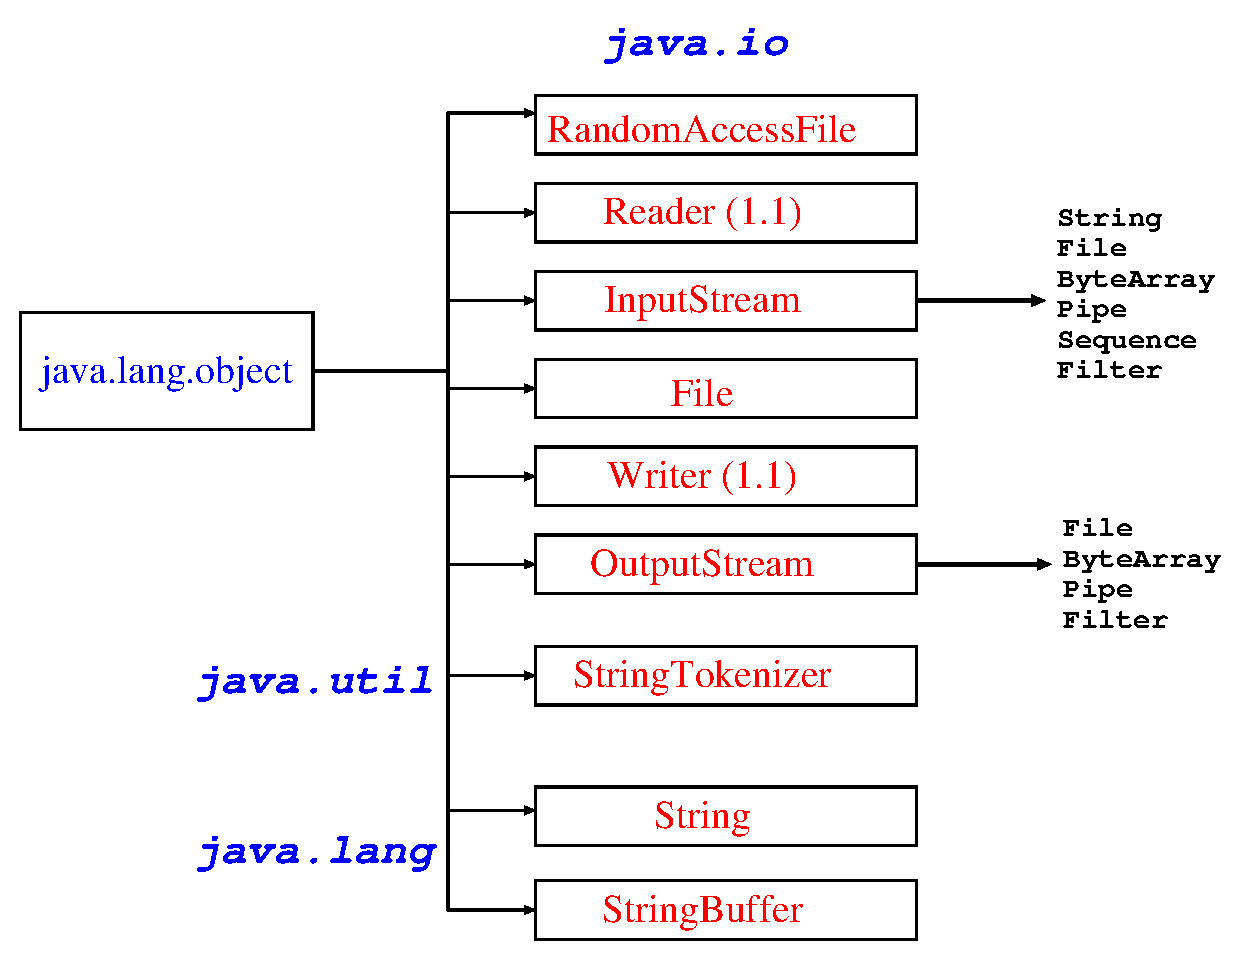
\includegraphics[width=\textwidth]{Figures/IOClasses.eps}
    \caption{Overview of the \texttt{io} package in Java 1.1 and 
      related classes.}
    \label{fig:FileIOClasses}
  \end{center}
\end{figure}
Except the \verb|Reader| and \verb|Writer| classes, all classes were
already introduced in Java 1.0. In Java 1.1 the two additional
classes just mentioned were added, because the \verb|InputStream|
and \verb|OutputStream| classes are using 8 bit characters and
the new classes use 16 bit unicode characters for international
languages support. In Java 2 only small changes have taken place
and therefore you can still stick to the Java 1.1 standard, but
should avoid using Java 1.0 I/O syntax if possible. 
This is also because the Java 1.1 Reader and Writer classes are
faster than the old ones.
Because File I/O almost always means handling strings, we have to
discuss this also in more detail. 

\paragraph{The concept of Streams}
The basic concept of input and output in Java is the \emph{stream}.
A stream is a collection of data in a certain order, which has to be
transported from a source to a sink. For example you want to
read data froma file, then you need a stream from the file, which
is the source, to a sink, which could be an array. This array can
of course be printed on screen to be read by the user. Thnis can also
be seen as a stream using the array as a source and the screen as the
sink. And really the \verb|System.out| method already familiar with
is derived froma stream (the \verb|PrintStream| class).

For any data communication from one ``point'' to another you
always have to use a stream in Java (like in C++). A nice feature
of streams is, that you can put two streams behind each other,
meaning to put the output of the first stream to the input of the 
second stream (see figure \ref{fig:ConnectingStreams}). 
\begin{figure}[htbp]
  \begin{center}
    \setlength{\unitlength}{.7cm} 
    \input{Figures/StreamsConnect.pic}
    \caption{Connecting two streams together to get advanced functionality.}
    \label{fig:ConnectingStreams}
  \end{center}
\end{figure}
This is the reason why modern programming languages
prefer to use streams to realize a very flexible input/output
API.  

You can even create very easily your own streams realizing very complex
filtering methods, but after reading this section you should be
able to understand the basics of streams and go to the online
API documentation and find your way through the classes yourself. 

\paragraph{ASCII Files}
But let us start with the most simple problem: We have an array 
of double values, for example the x coordinates of the discrete--time
random walk discussed afterwards and want to save them in a file
in the format \verb|time  x-coordinate|. To that end we need
to open a file for writing, write the array in it and close the file.

You probably would tend to look at the \verb|File| class for reading and 
writing files, but this class is only responsible for managing
files, directories and paths. We can use it to create a name
for our fiole to be created. For file access, you have to use the
\verb|Reader| and \verb|Writer| classes. So our small sample
program would look like:
\lstinputlisting{Listings_Java/FileWriteSimple.java}

First of all you realize that instead of just using the \verb|FileWriter|
class we ``pipe'' it to a \verb|BufferedWriter|, which buffers
the outgoing data between the disk and the memory. This is always
desirable and should therefore always be used. Otherwise you get
a very bad performance. Because it is inconvenient to remember all
this, we have written a convenience class in our \verb|simulation|
package. So you can have the same program, only lines 17-18 (or 19)
have to be changed to (and you have to import the simulation package,
see program \verb|FileWriteConvenience.java|.):
\begin{lstlisting}{}
    FileOut out = new FileOut( filename ); // open a buffered File stream
\end{lstlisting}
You can use a second argument to this constructor, which is a boolean
variable and indicates if ythe data should be appended to
the already existing file or not. The full syntax of the method
is therefore \verb|FileOut(String filename, boolean append)|.

Now we want to read the contents of the file back in. We use the
classes \verb|FileReader| and \verb|BufferedReader| as you may have
already guessed. The whole program looks like:
\lstinputlisting{Listings_Java/FileReadSimple.java}
Again you can use the convenience class \verb|FileIn| from the
simulation package, changing again the lines 17-18 (or 19) by:
\begin{lstlisting}{}
    FileIn in = new FileIn ( filename ); // open a File stream
\end{lstlisting}

Important remark:
\begin{quote}
Java always overwrites old files without notification as the default
behaviour! If you want to check if an old file already exists under
this name, you have to do that by yourself. If you want to append the
new data to the old one, use the second argument when creating a
new \verb|FileWriter| instance.
\end{quote}


\paragraph{Using a StringBuffer}
In the above examples and in all the \verb|System.out.println()| methods,
we make use of the concatenation operator \verb|+|. So here seems to
be the right place to discuss the fundamentals of string construction
a bit more in detail.

Often you are in the need of constructing a string from scratch, by
putting lots of small pieces (strings) together. Actually the same
problem as concatenating strings for (formatted) output. You could
always use the Lava Rocks methods, here especially the \verb|sprintf()| 
method explained in the next apragraph and in section \ref{sec:Symphony}.
But here we want to discuss how this can be implemented in  core Java.

The basic feature enabling string concatenation is the concept of a 
\verb|StringBuffer|. This is a standard class in the \verb|java.lang|
package and contains methods to manipulate strings. The \verb|String|
class itself (also in the \verb|java.lang| package) provides basic
functionality for fixed (non-changing) strings. As I already
mentioned every time you use the concatenation operator, you are
implicitly using the \verb|StringBuffer| methods. 

If you want to create a string, which contains all the output you want
to write to a file in one string, you could use a \verb|StringBuffer|.
Here is the same class as above for writing a double array to a file,
but this time we use the \verb|StringBuffer| to create a string
containing all the output and write this string to the file.
\lstinputlisting{Listings_Java/StringBufferDemo.java}
Now you have to take care of the length of the buffer yourself,
but if there is not enough space left Java automatically
enlarges the buffer itself, so you do not have to care.

Using a \verb|StringBuffer| is much faster and much less memory
extensive than just the concatenation operator, if you are
interested in the final string. If you just use it for output
it does not matter.

\paragraph{Stream- and StringTokenizer}
These two classes in the \verb|java.io| and the \verb|java.lang|
packages respectivly can be used to split up a stream of
characters or a string into words. You can define the word
separator yourself, the default is a white space. It is very
convenient for analyzing keyboard inputs or sentences.
You get the next word by using the \verb|nextToken()| method.
The \verb|StringTokenizer| is very simple and the \verb|StreamTokenizer|
is much more flexible and powerful.

\paragraph{Formatting the output in a file}
A common problem for writing files is the form of the produced
output. Like in the case of formatted screen output, you can use
one of the C language motivated \verb|printf| methods supplied by the
Lava Rocks package (see section \ref{sec:LavaRocks}). But instead
of using \verb|printf()| you have to use \verb|fprintf()| this time.

If you are a (former) C programmer, you might miss the third
output version of the formatting methods: in Lava Rocks it is also called
\verb|sprintf()|. 

A simple example of these routines would be to save
a double array, which is e.g. the x-coordinate of a particle, and 
the corresponding time in a file.
\lstinputlisting{Listings_Java/FileSaveFormatted.java}

\paragraph{Binary Files}
We are now familiar with writing ASCII files, but sometimes it is
necessary to write or read files in binary format, where the 
values are stored in the way they are kept in memory of the computer.
This makes it faster and most of the time it produces smaller
output files than using ASCII output.

The difference to other languages, where you have these two choices
too, is that in Java on all platforms the binary format is the
same, when it is saved. So here you do not have to mind using 
binary data files on different machines and operating systems as
long as you stick to Java.

All of the basic I/O classes implement writing bytes to a stream,
so you could actually use them. But there are two classes, which 
already implement the conversion of the different data types to 
a series of bytes and write these bytes to the desired stream.
The first one is \verb|DataInputStream| and the second one is
the \verb|DataOutputStream| class. They implement methods like
\verb|writeDouble()| (\verb|readDouble|), \verb|writeBoolean()|
(\verb|readBoolean()|), etc. There are also methods for
writimg strings (\verb|readLine()|) in these two classes, but
avoid them, because they do not convert the byte stream correctly
to character streams. Instead use the above discussed writer and reader
classes. 

As an example we look at the same example as above and write 100 
double variables to a file, so the file will be 800 bytes long
(on all computers and operating systems).
\lstinputlisting{Listings_Java/FileBinary.java} 
Please note that we have used unbuffered I/O here and for your
applications you should always use buffered I/O by inserting
a \verb|BufferedInputStream| (\verb|BufferedOutputStream|) between
the two streams used in the listing.

This paragraph was the way to write files introduced in Java 1.0,
the Reader and Writer classes were first introduced in Java 1.1.
There are also classes to convert the old streams to the new reader/writer
streams (classes). The \verb|InputStreamReader| class converts
an \verb|InputStream| 
to a \verb|Reader| class and the \verb|OutputStreamWriter| class 
converts an \verb|OutputStream| to a \verb|Writer| class.


\paragraph{Handling Files -- The File Class}
Sometimes you need to delete, rename or copy files or must check
if a file is already there or you have to seek in directories.
For all these problems you have to refer to the \verb|File| class 
(since Java 1.1) of
the \verb|java.io| package. Take a look at the extensive list
of methods available in this API and you will certainly find
something suitable. 

As a short example we want to discuss how show how to check if
a file with a certain filename is already available and 
how to handle directories and files therein.
\lstinputlisting{Listings_Java/FileCheck.java}

\paragraph{Direct File Access}
Since Java 1.1 
there is also a class called \verb|RandomAccessFile|, which is for
creating and accessing files directly. This means you can store
kind of data records and position the file exactly to a certain
record instead of reading the whole file sequentially. Because
in scientific applications this kind of file access is rather
seldom, we do not discuss this feature. You have to consult the
online API documentation for details. 

\paragraph{Redirecting Standard Input and Ouput}
You can redirect the standard output, input or error
to a file for example or whatever you like (since Java 1.1). 
This is of great use,
because often you run long simulations and want to save the
standard output or error to a file for later use. This can be
done easily on UNIX systems, but still you have to do it manually.
In Java you just use methods from the \verb|java.lang.System| class.
For example to redirect the standard output and error to a file
called \verb|Standard.out| of a program, use:
\lstinputlisting{Listings_Java/RedirectStandard.java}
The similar method for the standard input is called
\verb|System.setIn(InputStream)|.

\paragraph{Compressing Files}
File compression is not only important for transfering files or applets 
across the internet, it is also of concern for many scientists, who have
large data sets and have to write these sets to disk for 
postprocessing. 

Since the advent of the zlib compression library\footnote{%
\href{http://www.zlib.org}{http://www.zlib.org}} freely available under
the GNU license, it is pretty easy to use compression in your 
own programs in Fortran or C. But in Java the compression library is 
already made available in the standard Java API \verb|java.util.zip|.
As the name suggests not only the zlib compression algorithm used
in the famous GZIP program -- mostly used on UNIX systems using the
\verb|.gz| ending -- but also the algorithm of the famous zip
program -- mostyl used on Windows based systems and has the ending
\verb|.zip| -- is available in Java directly.

The only drawback is that it is implemented on top of the old
Java 1.0 I/O API and sometimes you have to mix the old Java 1.0
and the new Java 1.1 I/O syntax. 

The most easy interface is the GZIP one, so for most applications you 
should use GZIP. The Zip interface allows for multiple program 
compression in one file, but it is more cumbersume to use. Because
most of the time you have to compress a single stream of data, we
explain only the GZIP interface.

Let us discuss the probelm ofg saving an array to a file again, but
this time we want to store them compressed as a GZIP file.
\lstinputlisting{Listings_Java/GZIPSaveArray.java}
The first part stores it as a binary GZIP file \verb|test.bin.gz|
and you will see that it
does not save a lot of memory, because we are storing an array with random
numbers, which is already (almost) best represented by the binary
format. The second part produces an ASCII GZIP file \verb|test.asc.gz|,
which is much smaller than the uncompressed file. You can check this by
using the GZIP utility and uncompress the files. 

Reading of GZIP files works the same, you just have to use
the \verb|GZIPInputStream()| constructor and all the file I/O works
like usual file handling.

We have also implemented convenience classes for these complicated
structures to open a GZIP file for writing and reading. They are
called \verb|GZFileOutBin()| (\verb|GZFileOutAscii()|) and
\verb|GZFileInBin()| (\verb|GZFileInAscii()|) and are used like
the ones without compression. You can also take a look at the
program \verb|GZIPReadArray.java|.

\paragraph{Reading Files into Applets}
Because of security reasons there is (almost) no way of reading files or
writing files from within an applet. One way of doing it would be
to use the security features of Java. In this case the browser has 
to tell the applet explicitly that it is allowed to do file I/O. This
can be accomplished by signing an applet, prepared in a jar file. Then
the browser can check the signature and if the browser setup allows
file I/O for this signature it works.

A second way would be to use the network features of Java and
access a file from a FTP server, probably the same computer
the applet was coming from. Of course there is still the problem
of a password to be transmitted unsecurely to the FTP server, but
it is fairly easy to setup. The code to use is a freely available
program called \verb|LinLyn.java|. We have included the code in
our simulation package. The documentation is included in the Java file
or you can study the simulation package documentation. 

%%%%%%%
\subsection{Exception Handling in Java}
We have made extensive use of exceptions in the last section, but
now we have to understand what we did there. Exceptions are
``thrown'' if an exceptional condition or error occurs in a part
of a Java program. This can be a division by zero, a file not
found error or something else, which the JVM does not know 
how to handle. So it is up to you to write code, which takes
care of unusual conditions, which is called catching an exception 
-- the most common situations are already
caught by the standard Java implementation. 

If a piece of code produces an exception it is checked if the
code block surrounding the exception producing point is able
of handling the exception. If not, the exception is propagated
up to the next higher (calling) code block (method, class, etc.).
If none of the code up to the main method catches the exception,
an error message is shown on the command line and the program stops
with a stacktrace showing the last commands executed. This propagation
is a great simplification, because you can catch all of the exceptions
in one place and not distributed through the whole class hierarchy.

The exception handling is located in the \verb|java.lang.Throwable| class.
Exceptions are objects and there are two types: Errors and Exceptions.
Errors are usually not recoverable and the program has to exit with
an error message. From exceptions you can recover, e.g. 
``Array out of Bounds'', or ``IO Exception'', etc. The exceptions,
which are automatically caught are the \verb|RuntimeExceptions|.

The way of handling exceptions is easily seen in the above examples
about file I/O. You put the code, which can throw an exception in a
\verb|try { }| clause and use the \verb|catch() {}| clause afterwards
to define what has to be done, if an exception occurs in the try block.
\begin{verbatim}
try {
   // Code which throws exceptions.
} catch ( java.lang.Throwable e ) {
   // Code which catches/recovers from exceptions.
} finally {
   // Code which should be executed, no matter if an exception
   // occured or not, before global catching of the exceptions 
   // takes place.
}
\end{verbatim}
The \verb|java.lang.Throwable| keyword in the catch clause has to be
exchanged by one of the exceptions in table \ref{tab:Exceptions}. 
\begin{table}[htbp]
  \begin{center}
    \begin{tabular}{lcp{.6\textwidth}}
      Exception name & RTE & Ocurrence/Reason \\\hline
      IOException & N & Some IO problem (has lots of subclasses). \\
      ArrayIndexOutOfBoundsException & Y & array is out of bounds \\
      ArtihmeticException & Y & Integer division by zero \\
      NullPointerException & Y & If a \verb|null| instead of an object is used\\
      NegativeArraySizeException & Y & if you trie to create a negative sized array\\
    \end{tabular}
    \caption{Some of the important exceptions in the 
      \texttt{java.lang.Throwable} class. A detailed list is in the 
      API documentation. RTE means \texttt{RuntimeException} and therefore
      do not have to be catched.}
    \label{tab:Exceptions}
  \end{center}
\end{table}

Instead of explicitly catching exceptions you can also just
write \verb|throws IOException| after the class definition, before
the actual code. Then the exceptions are handed to the next higher 
instance and if there is no calling class anymore an error is
displayed. With this you can propagate all your exceptions to the
parent class of all of the classes and catch the exceptions there.

If you ask how do you know what exceptions to catch (if some of the
code is not written by you or is very complex), there are only
two possibilities: read the whole code and look for exeptions, which
can be thrown by it or wait for the exceptions to occur on the
standard output. 

You can even use your own exceptions very easily by using the keyword
\verb|throw| and your own name of an exception. That is an easy way
of handling exceptional conditions in your own code, like energy
turns zero or step size/accuracy gets too large, e.g.
\begin{verbatim}
  try {
       energy = newEnergy(energy);
       if (energy == 0 ) {
           throw  new EnergyZeroException(); 
       }
  } catch (EnergyZeroException e) {
       // do something about zero energy
  } catch (OtherExceptions e) {
       // maybe another exception to be caught
  } finally {
       // Always do something here, even if a certain exception
       // has been thrown, but not catched yet
  }
\end{verbatim}


%%%%%%%%%%%%
\subsection{The Discrete--Time Random Walk}
A drunkard leaves a pub. His house is at the end of a straight
street. Each time  he moves he walks one
step to the direction of his home  or one step in the opposite direction
with equal probability. The question we want to consider in this 
subsection is: What is the probability for the drunkard to be at 
home in $r$ steps? 

In a more formal language we want to associate with each step
a stochastic variable $X_i$ ($i=1,\ldots,r$) assuming only the 
values $+1$ and $-1$ with probability $1/2$ each. If he starts at
$n=0$, all possible positions are integers $-\infty < n <
\infty$. The position after $r$ steps will be
\begin{equation*}
Y = X_1 + X_2 + \cdots + X_r.
\end{equation*}
It is easy to check that $\langle Y \rangle = 0$ and since
the steps are mutually independent
\begin{equation*}
\langle Y^2 \rangle = r \langle X^2 \rangle = r.
\end{equation*}
The above relation expresses the very typical behaviour of a 
diffusive process: The mean squared displacement is proportional 
to the number of steps. To put it differently the variance of the 
mean of the velocity tends to zero  for long times
\begin{equation*}
\left\langle \left( \frac{Y}{r}\right)^2\right\rangle =
\frac{1}{r} \longrightarrow 0 \quad \text{as} \quad 
   r \longrightarrow \infty.
\end{equation*}

In order to find the probability distribution of $Y$ we make use
of the characteristic function
\begin{equation*}
G_Y(k,r) = [G_X(k)]^r = [\frac{1}{2}\exp(ik) + 
                   \frac{1}{2}\exp(-ik)]^r.
\end{equation*}
The probability that $Y$ has the value $n$ is the coefficient
of $\exp(ink)$
\begin{equation*}
p_n(r) = \frac{1}{2^r} {r \choose {\frac{(r-n)}{2}}}.
\end{equation*}

In order to make clearer these concepts we want to write a program 
to simulate the random walker in discrete time steps. The program
is called {\sf rwdt} and its listing can be seen below.

\subsubsection{Listing of the program rwdt.m}

\inputlisting{./Listings/rwdt.m}

In the program we have obviously to generate an integer valued random 
variable which can assume with equal probability the values $+1$ 
and $-1$. One way of generating an $n$--dimensional vector $x$ of 
such random numbers is
\begin{verbatim}
x = sign(rand(n,1)-0.5)
\end{verbatim}
We run the program for 1000 steps, i.e., we choose the parameter 
$nstep=1000$.
Two realizations of the one--dimensional random walk can be seen 
in Figs. (\ref{F_RWDT_1}) and (\ref{F_RWDT_2}). 
\begin{figure}
\label{F_RWDT_1}
\includegraphics[width=10cm]{./Figures/f_rwdt_1.eps}
\caption{One realization of a one--dimensional random walk.}
\end{figure}

\begin{figure}
\label{F_RWDT_2}
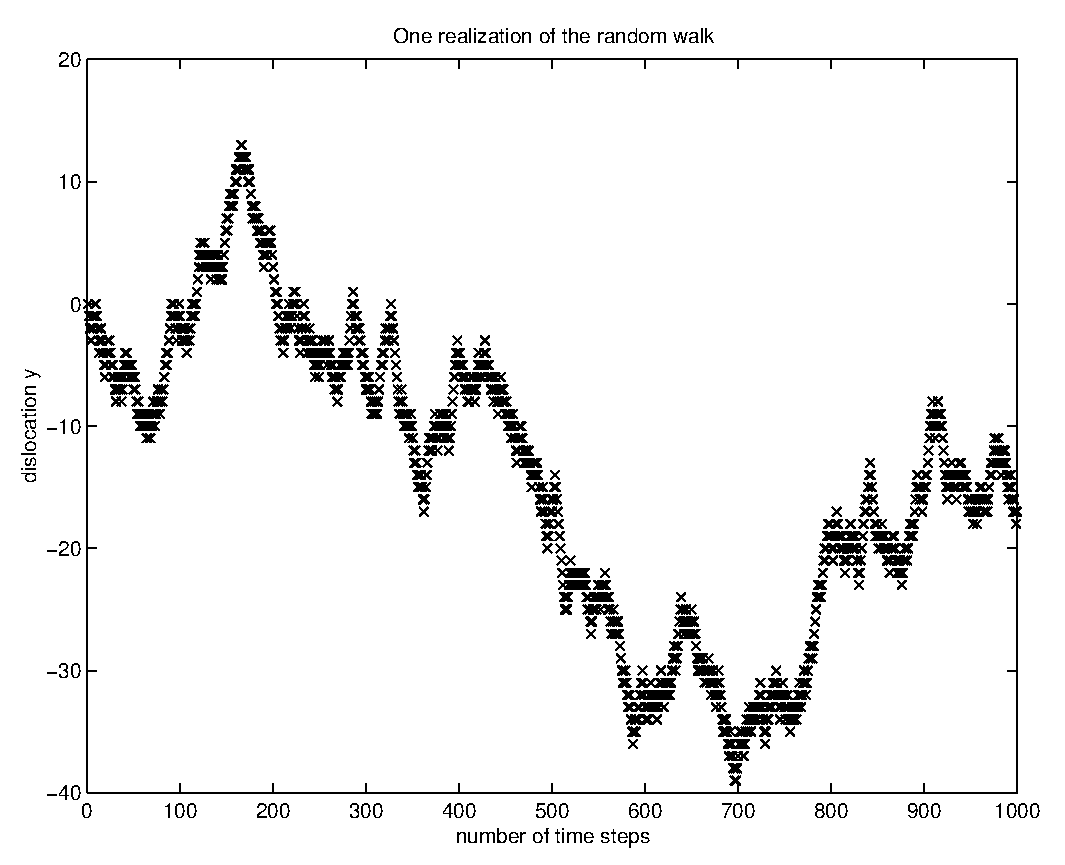
\includegraphics[width=10cm]{./Figures/f_rwdt_2.eps}
\caption{Another realization of a one--dimensional random walk.}
\end{figure}

In order to check the theoretical prediction that the mean square
displacement is proportional to the number of steps we generalize the program
{\sf rwdt} to allow for the generation of more realizations and 
the estimation of the mean value and variance. The new program is called 
{\sf rwdtn} and generates {\sf nreal} realizations of the 
stochastic process.
Its listing can be seen below.

\subsubsection{Listing of the program rwdtn.m}
\inputlisting{./Listings/rwdtn.m}
We run the program for $nstep=100$ and $nreal=1000$. The estimated
mean value of 0.274 and the estimated variance of 103.304 are in quite
good agreement with the theoretical expected vales of 0 nd 100, respectively.
It is interesting to look also at the distribution of the end points of 
the random walk. This can be seen in Fig. (\ref{F_RWDTN}).
\begin{figure}
\label{F_RWDTN}
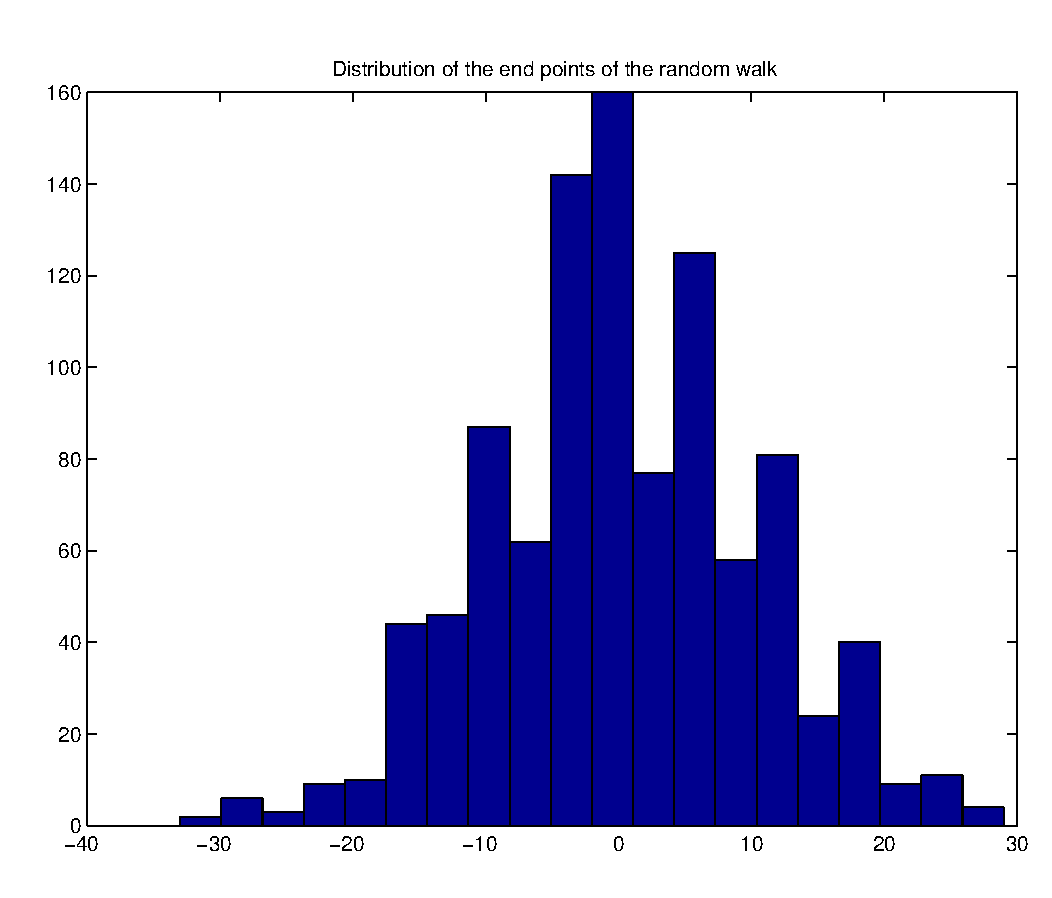
\includegraphics[width=10cm]{./Figures/f_rwdtn.eps}
\caption{The distribution of the end--points of the one--dimensional 
random walk. the program {\sf rwdtn} was run for nstep=100 and 
nreal=1000.}
\end{figure}
\subsection{Generation of Gaussian Random Numbers}
As a simple demonstration of the central limit theorem we want to 
generate Gaussian distributed random numbers by adding uniformly 
distributed ones.

We know that uniformly distributed random numbers on the interval
$[0,1)$ have $p(x) =1$ for $x\in[0,1)$. Then it is easy to show 
that 
\begin{equation*}
\langle X\rangle = \frac{1}{2}
\end{equation*}
and
\begin{equation*}
{\rm Var}(X) = \int_0^1 x^2 dx - \langle X^2\rangle = \frac{1}{3} 
        -\frac{1}{4} = \frac{1}{12}.
\end{equation*}
Now let us consider the transformed random variable $X'$
\begin{equation*}
X' = (X - \frac{1}{2})\sqrt{12} \sigma
\end{equation*}
which has mean $0$, variance $\sigma^2$, and is uniformly 
distributed on the interval 
$[-\frac{1}{12} \sqrt{12} \sigma, \frac{1}{12} \sqrt{12} \sigma].$
Let us now draw $N$ such random numbers $X'_1,\ldots, X'_N$
and let us construct
the new stochastic variable $Z$
\begin{equation*}
Z= \frac{1}{\sqrt{N}} (X'_1 + \ldots + X'_N).
\end{equation*}
Then the central limit theorem states that the variable $Z$ is a Gaussian
variable with mean $0$ and variance $\sigma^2$.

With the help of the program {\sf cltgen} we want to demonstrate 
that already for $N=12$ we get Gaussian distributed random numbers
in a very good approximation.

\subsubsection{Listing of the program cltgen.m}
\inputlisting{./Listings/cltgen.m}

In Fig. (\ref{F_CLTGEN}) we see the distribution of the Gaussian 
random numbers generated with the help of the program {\sf 
cltgen}. The number of random numbers $Z$ was chosen to be 1000.
\begin{figure}
\label{F_CLTGEN}
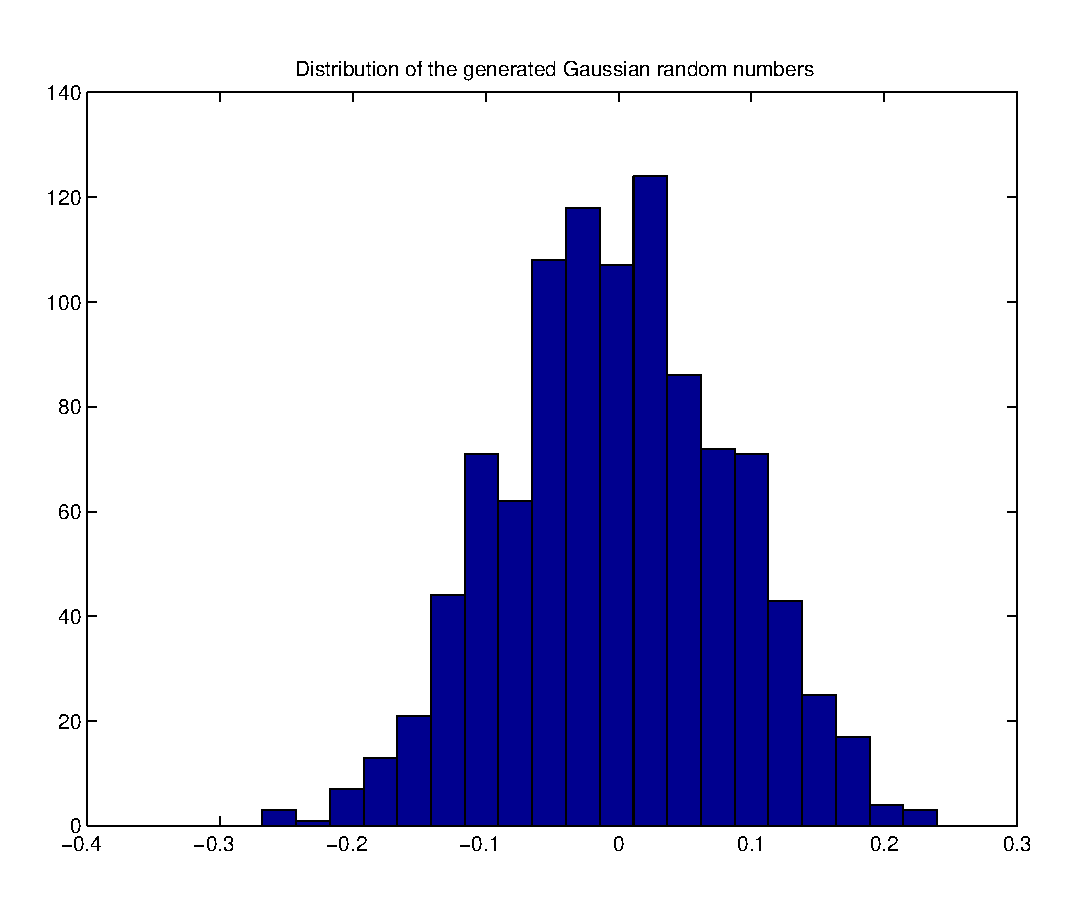
\includegraphics[width=10cm]{./Figures/f_cltgen.eps}
\caption{The distribution of the Gaussian random numbers generate
with the help of the program {\sf cltgen}. The number of random numbers 
drawn was chosen to be $n=1000$.}
\end{figure}

\subsection{Estimation}
{\em Experimental data are random numbers!} An experiment provides
realizations of some random variable $X$. We call an $N$--fold
realization of $X$ a sample of size $N$. It is of fundamental
importance to distinguish between the estimate for the mean and the
variance made on the basis of the sample, which we will denote by $m$
and by $s$, respectively and the corresponding quantities for the
(infinite) underlying population, the ensemble.

Of course, estimates should be unbiased, i.e., for very large samples
the estimate based on the sample size $N$ should converge to the
ensemble averages.

\subsubsection{Mean Values}
Let us consider $N$ copies $X_1, \ldots, X_N$  of a random variable
$X$ and let us build the new stochastic variable
\begin{equation*}
Z = \frac{1}{N}(X_1 + \cdots + X_N).
\end{equation*}
$Z$ is the mean value of the $N$ realizations. Assuming that the $X_i$
are uncorrelated we obtain for the cumulants of $Z$
\begin{equation*}
\kappa_n(Z) = \frac{1}{N^n} \sum_{i=1}^N \kappa_n(X_i) =
      N^{-n+1}  \kappa_n(X).
\end{equation*}
In particular we have
\begin{eqnarray*}
\kappa(Z) & = & \langle Z \rangle = \langle X \rangle \\
\kappa_2(Z) & = & {\rm Var}(Z) = \frac{1}{N} \kappa_2(X) = \frac{1}{N}
                  {\rm Var}(X) \\
\kappa_n(Z) & = & O(N^{-2}) \;\;\; {\rm for} \;\; N>2.
\end{eqnarray*}
In other words the mean value of $Z$ is a random variable with a
distribution which has the same mean value as $X$, but with a variance
which is smaller by a factor of $N$. Up to terms of the order
$O(N^{-2})$ the distribution of $Z$ is Gaussian.

\subsubsection{Estimating Mean and Variance}
Let us consider to have the sample $x_1, \ldots, x_N$. A natural
estimator of the mean value $\mu$ is the sample mean
\begin{equation*}
m= \frac{1}{N} \sum_{i=1}^N x_i.
\end{equation*}
An estimate for the variance could, in analogy, naturally assumed to
be
\begin{equation*}
  \bar{\sigma}^2 = \frac{1}{N} \sum_{i=1}^N (x_i -m)^2.
\end{equation*}
Unfortunately, the above estimator is biased, because we make use of
the already known $m$ instead of the unknown $\mu$. As can easily be
seen
by adding and subtracting $\mu$ in each term in the above equation we
get
\begin {eqnarray*}
 \bar{\sigma}^2 &=& \frac{1}{N} \sum_{i=1}^N [x_i - \mu -(m-\mu)]^2 \\
                & = & \frac{1}{N} \sum_{i=1}^N (x_i - \mu)^2
                              -2(m-\mu)\frac{1}{N} \sum_{i=1}^N (x_i
                                   - \mu)
                           +(m-\mu)^2 \\
               & = & \frac{1}{N} \sum_{i=1}^N (x_i - \mu)^2 - (m-\mu)^2.
\end{eqnarray*}
Now, by taking expectation values averaging over an infinity of samples
of size $N$ we have
\begin{eqnarray*}
E[\bar{\sigma}^2] &= & E\left[\frac{1}{N} \sum_{i=1}^N (x_i - \mu)^2
                                \right]
            - E\left[(m-\mu)^2 \right] \\
       & = & \sigma^2 - \sigma_m^2.
\end{eqnarray*}
If we assume, that there are no correlations we have $\sigma^2_m=
\sigma^2/N$, an unbiased estimate of $\sigma^2$ is
\begin{equation*}
s^2 = \frac{N}{N-1} \bar{\sigma}^2 = \frac{1}{N-1} \sum_{i=1}^N 
      (x_i - m)^2.
\end{equation*}
In computations, if the sample is large, rounding errors can be large
because $(x_i - m)$ is small. In
these cases it is convenient to use the 
"corrected two--pass algorithm" for $s^2$
\begin{equation*}
s^2 = \frac{1}{N-1} \left\{ \sum_{i=1}^N 
      (x_i - m)^2 - \frac{1}{N} \left[\sum_{i=1}^N 
      (x_i - m) \right]^2  \right\}.
\end{equation*}
The function of the additional second term which would be identically
equal to zero if $m$ were exact is to correct the rounding errors of
the first term \cite{PRESS}.

\subsubsection{Confidence Levels}
It is important to have also a quantitative characterization of the
goodness of the estimation. To this end we assign to every 
estimation a certain confidence interval, which is to be chosen in 
such a way that the true value lies within this interval at some
predetermined level of confidence. Since we know, by virtue of the
central limit theorem, that the mean value is Gaussian distributed
a criterion for the error can be directly derived from the 
geometric properties of the distribution. Assuming that the
mean value is $m$ and that the standard deviation is
$\sigma_m$ then the probability to find the true value in the
interval $[m-\sigma,n+\sigma]$ is given by the surface 
under a normal probability density
between  $\mu-\sigma_m$ and $\mu + \sigma_m$
\begin{equation*}
{\rm Prob}(\mu \in [m-\sigma,n+\sigma]) =
\int_{m-\sigma}^{m+\sigma} \frac{1}{\sigma \sqrt{2\pi}}
       \exp\left( - \frac{(x-m)^2}{2\sigma^2}\right)
       = 0.683.
\end{equation*}
Thus, in $68.3 \%$ of
samples a value lying within $\pm \sigma_m$  of the population mean
$\mu$ would be found. Conversely, there is $68.3 \%$ probability that
the interval $[m-\sigma_m, m+\sigma_m]$ contains the population mean.

In general we have...

\section{Beyond this Chapter}

%%%%%%%%%%%%%%%%%%%%%%%%%%%%%%%%%%%%%%%%%%%%%%%%%%%%%%%%%%%%%%%%%%
\section{Exercises}

\begin{Ex}
\label{Random-Number_Generator_Check}
\textbf{Random-Number Generator Check \cite[]{knuth2:81}} \\
To test the random number generator of Matlab, we calculate the first
10 moments of the distribution generated from \texttt{rand()}.
Compare these with the exact results for a uniform distribution.

Plot a histogram to check for a uniform distribution.

Use the Poker-Test for testing \texttt{rand}: Create many series of 5
random numbers between 1 and 13. Then count the fractions of hands
with two, three and four identical (numbers) cards. Compare the
result with the predictions:
\begin{center}
  \begin{tabular}{lrr}
hand & number of ways& probability\\\hline
all different (no pair) & 1,302,540 & 0.50117739\\
two of a kind & 1,098,240 & 0.42256903\\
three of a kind & 54,912 & 0.021128451\\
four of a kind & 624 & 0.000240096 \\\hline
Total number of possibilities & 2,598,960 & 1
\end{tabular}
\end{center}
For a rigorous check you have to use the chi-squared test for
your results. If you are interested, take a look at the book of D. Knuth.   
\end{Ex}

\begin{Ex}
\label{Galton_Board}
\textbf{Galton Board and Pascal Triangle \cite[]{whitney:90}} \\
Write a program to simulate a Galton Board on the computer.

\begin{center}
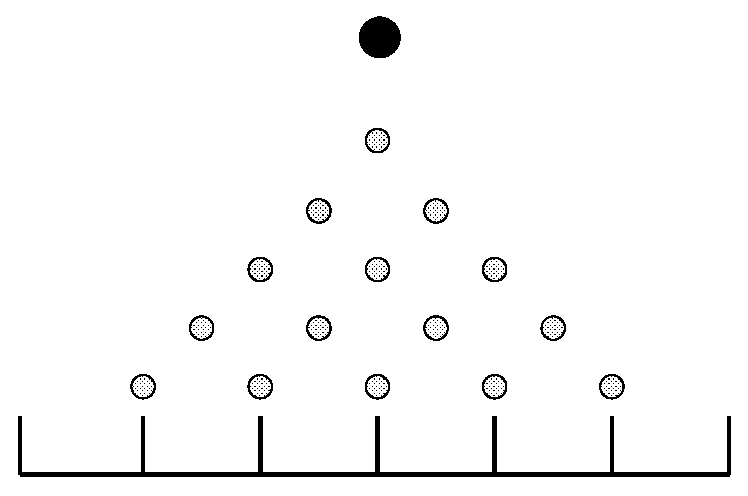
\includegraphics[height=4cm]{Galton_Board.eps}
\end{center}

That is a device where you introduce a ball at the top. The ball
falls down towards the bottom, bouncing off the pins to the right
or left at each level. The only random effect is the bouncing at
the pins at each level. The probability of bouncing to the right or
left is always $0.5$. Therefore it is a simple model for a symmetric
random walk in one dimension.

How can you extract the number of ways to get to one particular
box at the end of the board out of the estimated probabilities above?
What is the connection to the Pascal Triangle?

Change the program to simulate a asymmetric random walk in one
dimension.
\end{Ex}

\begin{Ex}
\label{Standard_Deviation}
\textbf{The Standard Deviation } \\
Compare the four possibilities to calculate the standard deviation
(or the variance):
\begin{enumerate}
\item using the definition: \\
  $$\sigma^2 = \frac{1}{N-1} \sum_{i=1}^N \left( x_i-\overline{x} \right)^2,
    \quad \overline{x} = < x > = \frac{1}{N} \sum_{i=1}^N x_i .$$
\item using the moments: \\
  $$ \sigma^2 = < x^2 > - < x >^2, \quad < x^2 > = \frac{1}{N} 
     \sum_{i=1}^N x_i^2 .$$
\item using the formula (\cite[]{scariano:91}):
  $$ \sigma^2 = \frac{1}{N^2} \sum^N_{\substack{i=1 \\ i<j}} 
      \left( x_i-x_j\right)^2.$$
\item using the corrected two-pass formula \cite[]{recipes}:
  $$ \sigma^2 = \frac{1}{N-1} \left\{\sum_{i=1}^N (x_i-\overline{x})^2
     -\frac{1}{N} \left(\sum_{i=1}^N(x_i-\overline{x}) \right)^2 \right\}.$$
\end{enumerate}
The first and the second method require the computation of the first or
the first and the second moments. The third moment doesn�t require any
precomputed values at all and the last one uses again only the first moment.
The last one corrects for the roundoff errors, encountered when using large
sample sizes. The last one is analytically exact only if $\overline{x}$
would be exact. 

Write a program including all four methods and compare the results.
Find out which method the Matlab function \texttt{std} uses.
Check the calculation with a uniform, a normal and a Cauchy (Lorentz)
distribution. Can you find an example where the two-pass algorithm
is superior to the other ones?

By the way, the variance is not the only value to estimate the
spreading of a sample. Statisticians often use the estimate
$$ \text{adev}\, = \frac{1}{N} \sum_{i=1}^N \left| x_i - \overline{x}\right|$$
as a measure for the distribution width around the mean value.
\end{Ex}

%%%%%%%%%%%%%%%%%%%%%%%%%%%%%%%%%%%%%%%%%%%%%%%%%%%

{\bf Exercise 2} Random variable transformation theorem: (a) Consider 
the linear transorm of X: Y=bX+c. (b) the log--normal 
distribution.
Lit. Gillespie, Am. J. Phys. 51 (1983) 520.
lichkeitstheoretische Grundbegriffe; typische 
Verteilungen (Poisson, Gauss, Binomial); 

%%%%%%%%%%%%%%%%%%%%%%%%%%%%%%%%%%%%%%%%%%%%%%%%%%%%%%%%%%%%%%%%%%


\bibliographystyle{peter}
\bibliography{V_98,simulit}

%%% Local Variables: 
%%% mode: latex
%%% TeX-master: t
%%% End: 


%%% Chapter 3 
%%%%%
%%%%% Chapter 3
%%%%%
\chapter{Simple Sampling of Probability distributions Using Random numbers}
This Chapter is devoted to the following question: How can we 
generate sequences of random numbers which are distributed 
according to some given distribution?

A simple answer to this question would be to exploit some 
intrinsically random physical process. For example, one could 
record a sequence of the decay times of some radioactive substance 
and use this truly random sequence of numbers in a Monte--Carlo
simulation. Although tables of millions of such true random 
numbers exist in practice this approach turns out not to be very
practical. Monte--Carlo simulations need very long sequences of 
random numbers, so that we have to find more efficient ways to 
generate them. In order to satisfy this requirement we have to 
be satisfied with the use of so--called pseudo--random numbers.
Pseudo--random numbers are generated numerically with the help of 
some simple algorithm on some computer. Consequently, they are
reproducible. This is, however, not a drawback. In fact, the 
reproducibility may be very useful if we want to check our 
simulation algorithms. 

Pseudo--random numbers are, the name already underlines it, not 
truly random. However, their statistical properties are very 
similar to the statistical properties of truly random numbers. So, 
for all practical purposes pseudo--random numbers appear to be 
random. Let us now see how such pseudo--random numbers can be 
generated.

\section{The generation of uniformly distributed random numbers}
We will begin with the generation of uniformly distributed random 
numbers on the interval $[0,1)$. In the following we will often 
omitt the prefix pseudo. 

The best known algorithm for the generation of uniformly 
distributed random numbers is the linear congruential method, 
which given an initial integer "seed" value $I_1$ produces random 
integers recursively from the formula
\begin{equation*}
I_{n+1} = (aI_n +c) \mod M,
\end{equation*}
where $a$, $c$, and $M$ are integer constants which have to be 
chosen appropriately. 
The randomness of the above algorithm results from the fact that 
after some multipications with $a$ the result exceeds $M$ and is 
consequently truncated. Since the integers $I_n$ lie between 1 and 
$M$ a random number $R$ uniformly distributed 
between 0 and 1 is obtained as
\begin{equation*}
R = \frac{I_n}{M}.
\end{equation*}
Unfortunately, MATLAB does not have integer arithmetic so the above algorithm 
has to be implemented using the {\sf rem} (remainder) function 
instead of the modulo function. A corresponding code could be
\begin{verbatim}
I(n+1) = floor( rem(a*I(n) + c,M) ).
\end{verbatim}
In order to get familiar with this algorithm we want to generate a 
sequence of pseudo--random numbers for the following parameters:
we choose the multiplier to be $a=$, the increment $c=3$, and the 
modulo $M=8$. Obviously the longest period of random numbers will
have the length 8. The generation of the random sequences will
be achieved with the program {\sf trandom1}.

\subsubsection{Listing of the program trandom1.m}
%%%%% trandom1 %%%%%%%%%%%%%%%%
\begin{verbatim}
% trandom1 - Program to demonstrate the generation of random numbers
% using the linear congruential method
clear; help trandom1 %clear the memory and print header
seed = input('Enter the seed (1) - ');
m = input('Enter the modulus (8) - ');
a = input('Enter the multiplier (5) - ');
c = input('Enter the increment (1<=c<7) - ');
% Set starting value
R(1) = seed;
% Generate vector of m random numbers
for j=1:m
   R(j+1) =floor(rem(a*R(j)+c,m));
end
%R=R/M;
disp('The generated series is:')
disp(R)
plot(R,'x')
title('The series of generated random numbers');
xlabel('Term, i'); ylabel('Value');
\end{verbatim}
%%%%%%%%%%%%%%%%%%%%%%%%%%%%%%%%%%%%%%%%%%%%%%%%%%%%%%%%%%%%%%%

Run with the above parameters the program generates the sequence
\begin{equation*}
1, 0, 3, 2, 5, 4, 7, 6, 1, 0, 3, 2 \ldots
\end{equation*}
which has also been plotted in Fig. (\ref{F_TRANDOM1}).
\begin{figure}
\label{F_TRANDOM1}
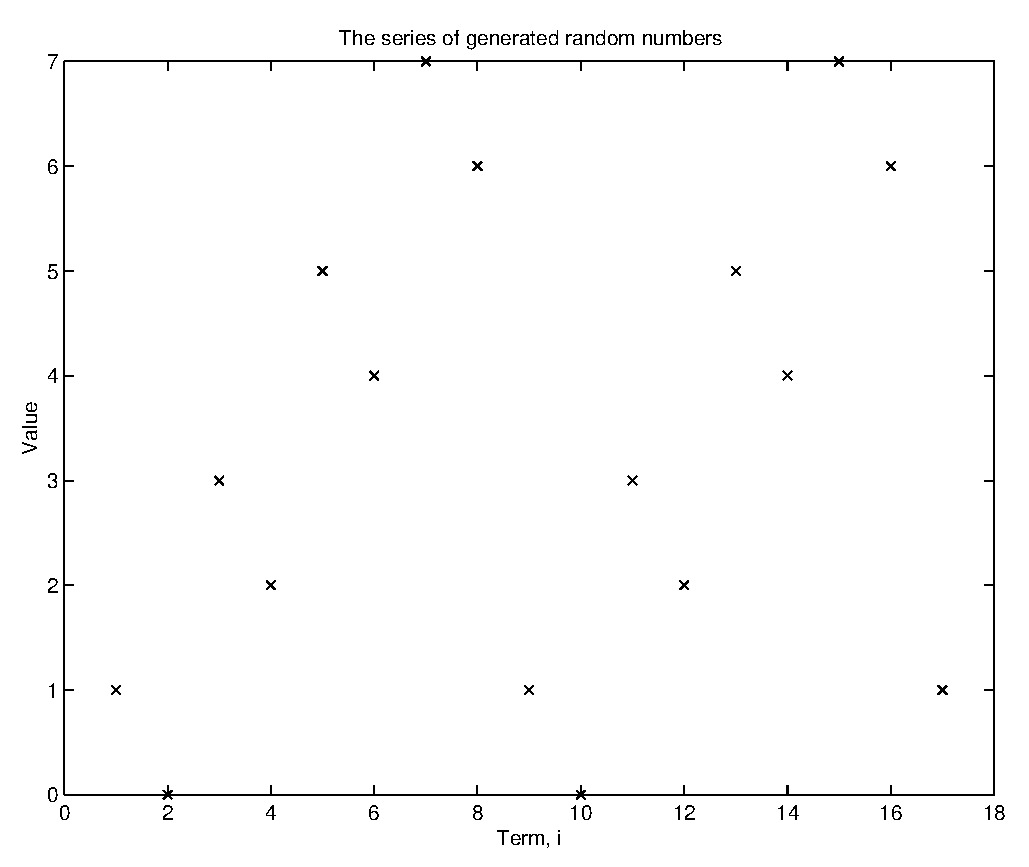
\includegraphics[width=10cm]{./Figures/f_trandom1.eps}
\caption{Successive values in a series of random numbers generated
for a=5, c=3, M=8. Note that the even numbers are always one less 
then the odd ones!}
\end{figure}
It might be instructive to run the program keeping the multiplier 
and the modulo fixed while changing the increment. The result of 
these runs are summarized in Table \ref{T_LCG}.

\begin{table}
\label{T_LCG}
\caption{Series of random numbers for the linear congruential 
generator of the form $I_{n+1} = (5I_n +c) \mod 8$}
\begin{tabular}{ccc} \hline
c &  $I_n$ & Period  \\ \hline
1 & 1,6,7,4,5,2,3,0 & 8 \\
2 & 1,7,5,3,1,7,5,3 & 4 \\
  & 4,6,0,2,4,6,0,2 & 4 \\
3 & 1,0,3,2,5,4,7,6 & 8 \\
4 & 1,1,1,1,1,1,1,1 & 1 \\
  & 2,6,2,6,2,6,2,6 & 2 \\
  & 3,3,3,3,3,3,3,3 & 1 \\
  & 4,0,4,0,4,0,4,0 & 2 \\
  & 5,5,5,5,5,5,5,5 & 1 \\
  & 7,7,7,7,7,7,7,7 & 1 \\
5 & 1,2,7,0,5,6,3,4 & 1 \\
6 & 1,3,5,7,1,3,5,7 & 4 \\
  & 2,0,6,4,2,0,6,4 & 4 \\
7 & 1,4,3,6,5,0,7,2 & 8
\end{tabular}
\end{table}
It is evident that a wrong  choice of the constants leads to a 
very poor random sequence.

It can be shown that (Knuth)  that in the case $c=0$ the full 
period, 1 to $M-1$ can be achieved by choosing $M$ as aprime 
number and for $a$, a primitive element modulo $m$, i.e., for all 
prime divisors, $p$, of $(M-1)$, 
\begin{equation*}
a^{(M-1)/p} {\rm mod} M \ne 1.
\end{equation*}
For the case of $c\ne 0$ the full period is obtained if the 
following three conditions are satisfied:

(i) $c$ and $M$ are relatively prime,

(ii) $a {\rm mod} p = 1$ for each prime factor $p$ of $M$,

(iii) $a {\rm mod} 4 = 1$ if 4 divides $M$.

It is evident that the greater the modulus the longer the period.
For example the MATLAB random number generating function uses
\begin{equation*}
a= 16807; c=0; M=2^{31}-1.
\end{equation*}
This chioce has been suggested by Park and Miller (Lit. Press).
The period of the generator is $2^{31}-2 \approx 2.1 \times 10^9$.
Another poupular popular random generator uses
\begin{equation*}
a= 65539; M=2^{31}-1; c=0,
\end{equation*}
and will be used in the following program {\sf trandom2.m}. There 
we will draw a number $n=xxx$ of random numbers using the linear 
congruential method. In the program we will check the quality of 
the generator by plotting the 1D, 2D, and 3D distribution of the 
pseudo--random numbers. The results of the test can be seen in 
Figs. (\ref{F_TRANDOM2_1}), (\ref{F_TRANDOM2_2}), 
(\ref{F_TRANDOM2_3}), and (\ref{F_TRANDOM2_4}).



\subsubsection{Listing of the program trandom2.m}
\begin{verbatim}
% trandom2 - Program to test random number generators
% The program makes use of the random number generator random1
clear; help trandom2; % clear memory and print header
% Enter dimension of random vector
n= input('Enter value of n-'); % 
% generate random vector
R1=random1(n);
% plot random vector
plot(R1)
title('random numbers'); xlabel('random variable');
disp('Histogram: press any keyboard key');
pause;
% plot histogram of random numbers
x=(0.05:0.1:0.95);
[m,xout] = hist(R1,x);
bar(xout,m)
xlabel('random number');
title('1D distribution: Histogram');
disp('2D plot: press any keyboard key');
pause;
% 2D plot: correlation of consecutive numbers
R2x=R1(1:2:n-1);
R2y=R1(2:2:n);
plot(R2x,R2y,'x')
title('2d distribution')
disp('3D plot: press any keyboard key');
pause;
% 3D plot: correlation of consecutive numbers
R3x=R1(1:3:n);
R3y=R1(2:3:n);
R3z=R1(3:3:n);
%R3=random1(n,3);
plot3(R3x,R3y,R3z,'x')
title('3D distribution');xlabel('Random number');
\end{verbatim}

\subsubsection{Listing of the function {\sf random1}}
%%%%%%%%%%%%%%%%%%%%%%%%%%%%%%%%%%%%%%%%%%%%
\begin{verbatim}
function R = random1(n)
% function to generate random numbers
a=65539;
M=2^(31)-1;
R(1) = 12345678;
for j=1:n-1
%   for i=1:n-1
   R(j+1) =floor(rem(a*R(j),M));
%end
end
R=R/M;
\end{verbatim}

\begin{figure}
\label{F_TRANDOM2_1}
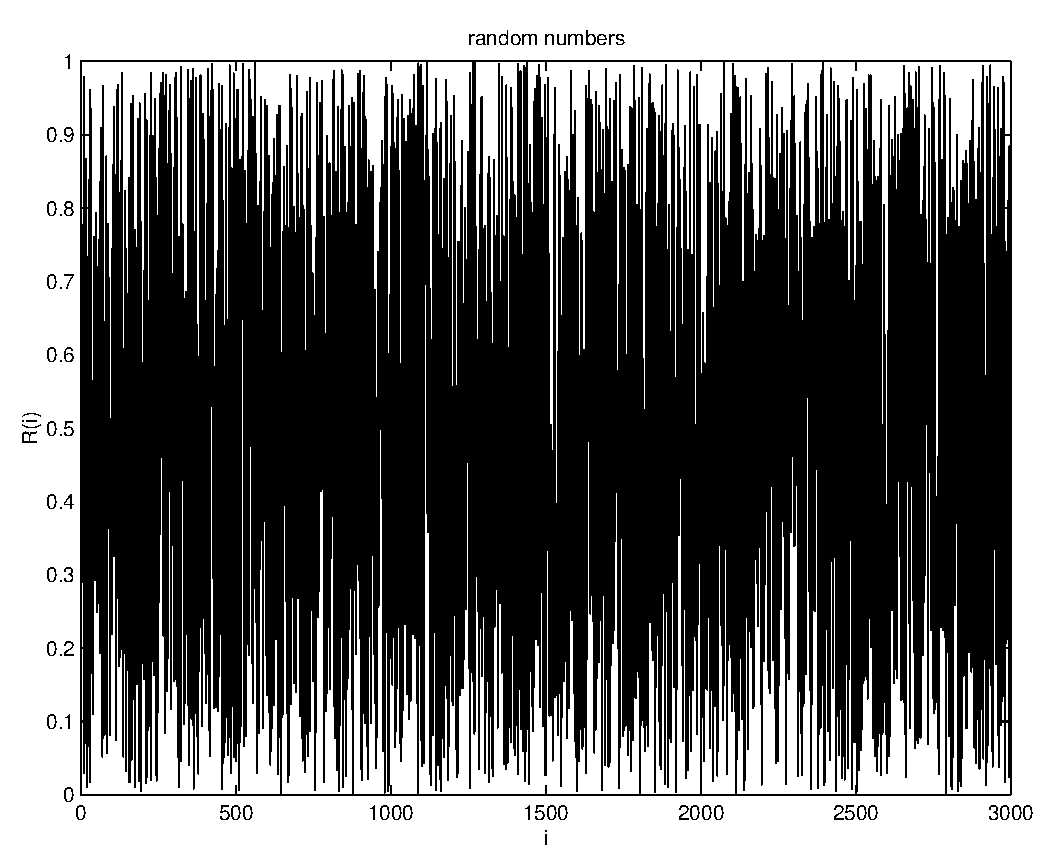
\includegraphics[width=10cm]{./Figures/f_trandom2_1.eps}
\caption{Successive values in a series of 3000 random numbers generated
for $a=65539$, $c=0$, $M=2^{31}-1$.}
\end{figure}

\begin{figure}
\label{F_TRANDOM2_2}
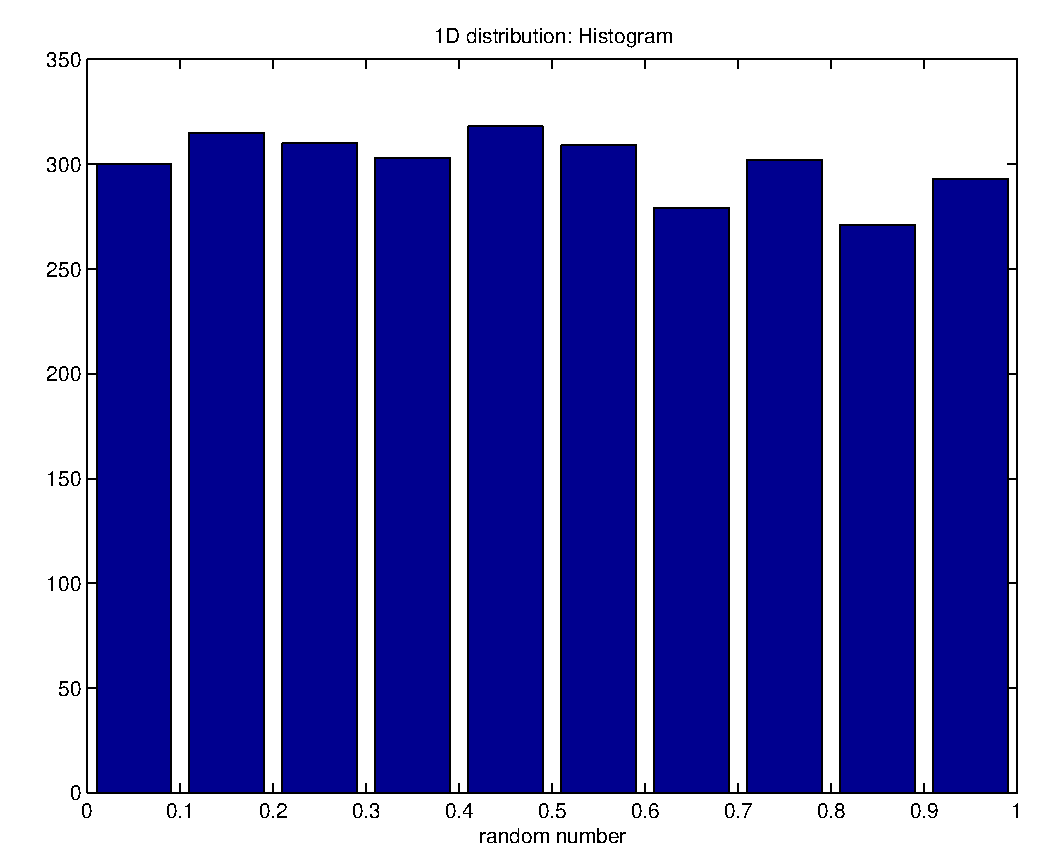
\includegraphics[width=10cm]{./Figures/f_trandom2_2.eps}
\caption{Histogram for a series of 3000 random numbers generated
for $a=65539$, $c=0$, $M=2^{31}-1$.}
\end{figure}

\begin{figure}
\label{F_TRANDOM2_3}
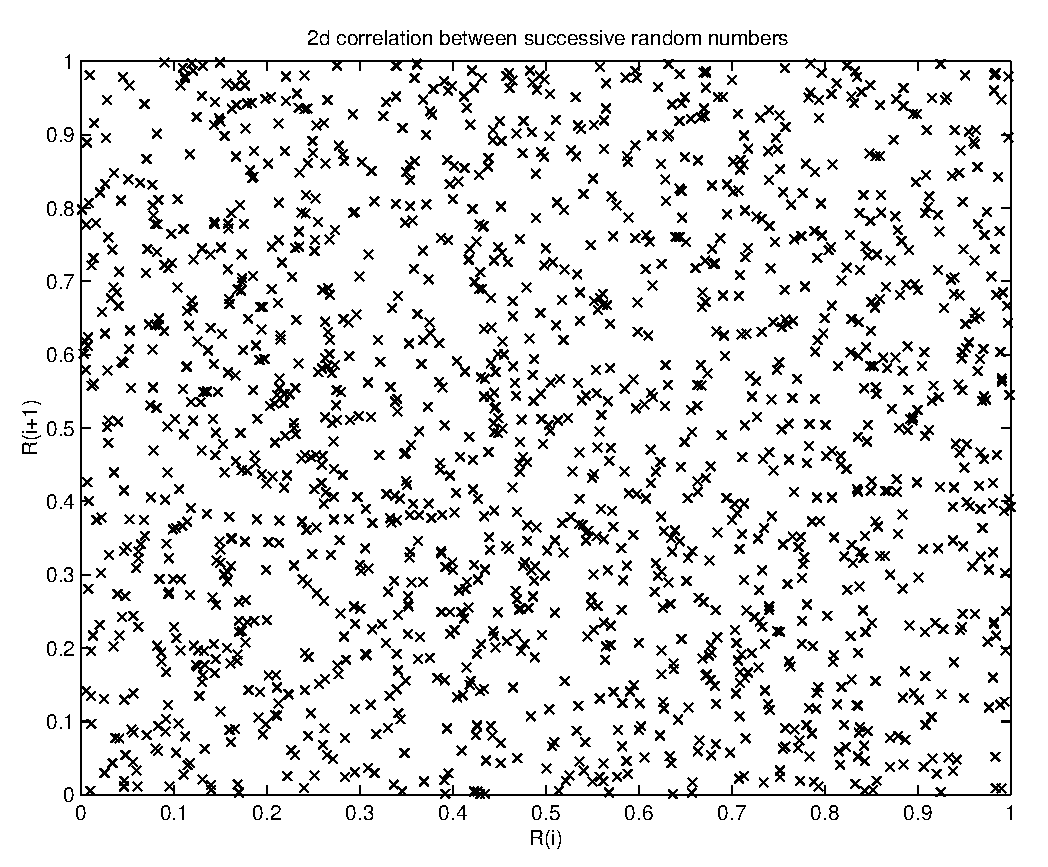
\includegraphics[width=10cm]{./Figures/f_trandom2_3.eps}
\caption{Correlation between successive values in a series of 3000 
random numbers generated for $a=65539$, $c=0$, $M=2^{31}-1$.}
\end{figure}


\begin{figure}
\label{F_TRANDOM2_4}
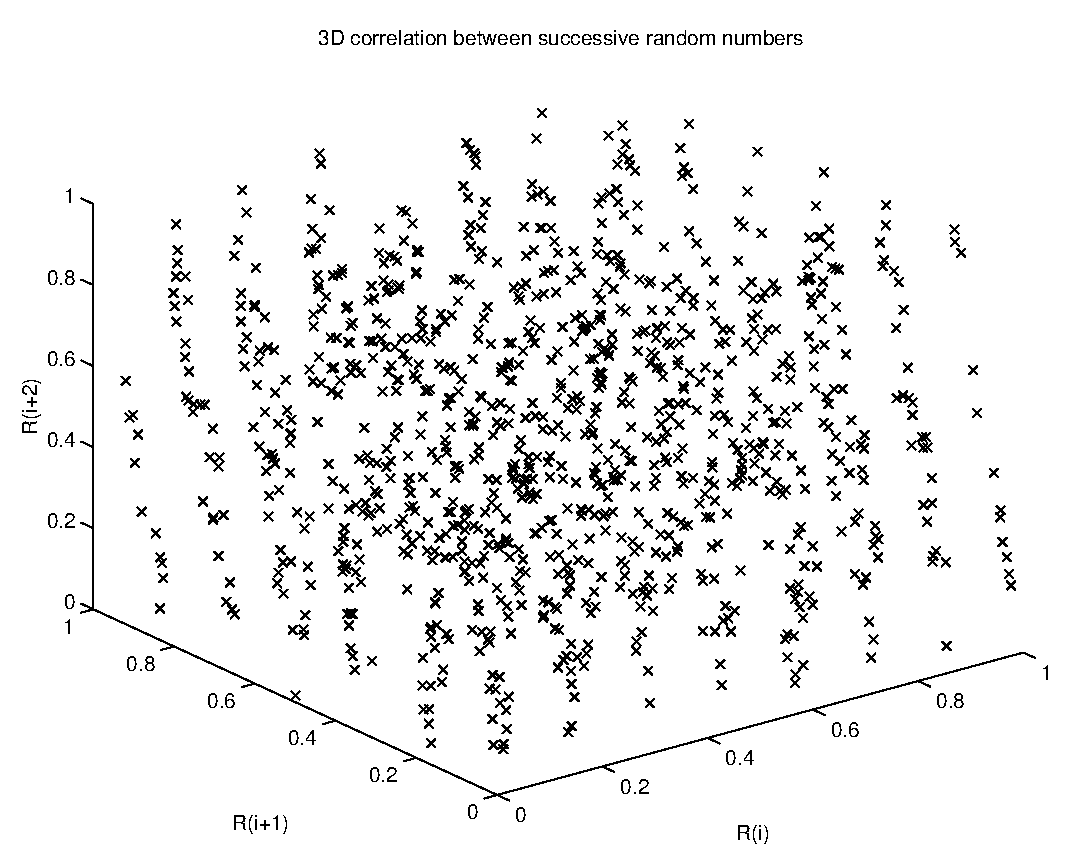
\includegraphics[width=10cm]{./Figures/f_trandom2_4.eps}
\caption{Correlation between successive values 
$R(i),R(i+1), R(i+2)$ in a series of 3000 random numbers generated
for $a=65539, c=0, M=2^{31}-1$.}
\end{figure}

The figures clearly reveal that the generator is not perfect.
In the exercise we will learn that choosing $a=16807$, the minimal
standard generator, 
significantly improves the performance. The performance of 
this minimal standard generator can be increased by shuffling
the output to remove low--order serial correlations (EXERCISE!!!!)
({\sf ran1} of Numerical Recipes).

In the book by Press et al. other "Quick and Dirty" linear 
congruential generators
are presented. Furthemore, serial correlations can be broken up by 
combining two linear congruential generators.

There are also other algorithms for the generation of random 
numbers: Shift--register generators (Lit: Kirkpatrick and Stoll), 
Fibonacci generators (lit: Knuth, James) or quasi--random numbers 
and we refer the reader to the original literature.

\section{The Transfomation method: Invertible distributions}
In the previous section we have learned how to generate random 
numbers with a uniform probability distribution, so that the 
probability $p(x)dx$ to generate a random number between $x$ and $x+dx$
is given by
\begin{equation*}
P(x)dx = \left\{ \begin{array}{ll}
                   dx & 0<x<1 \\
                   0   & {\rm otherwise}.
                  \end{array}
         \right.
\end{equation*}
With the help of the random variable transformation theorem it is easy
to transform uniform deviates into random numbers which are 
distributed according to invertible, one--to--one, distributions.
We know from Chap. 2 that if we take a uniform deviate $x$ and then 
transform it to a new variable $y(x)$ the probability distribtion
of $y$ is given by
\begin{equation}
p(y) = p(x) \left| \frac{dx}{dx}\right|.
\end{equation}
We want to derive a transformation which generates random numbers 
which are distributed according to a given
$p(y)$. Since $x$ is uniformly distributed the 
above equation reduces to
\begin{equation}
\label{INVERTIBLE}
\frac{dx}{dy} = p(y),
\end{equation}
which can be easily integrated
\begin{equation*}
x(y) = P(y) = \int^y p(y')dy'.
\end{equation*}
Hence, the transformation we are looking for is given by the 
inverse of $P(y)$. Thus, a random variable $Y$ with density $p(y)$
can be generated by uniform deviates trough
\begin{equation*}
Y = Y(X) = P^{-1}(X).
\end{equation*}
In the following we will apply this method to generate 
exponentially and gaussian distributed random numbers.

\subsection{Exponential distribution}
Let $p(y)= w\exp(-wy)$ for positive $y$. It follows from Eq. (\ref{INVERTIBLE})
that
\begin{equation*}
\frac{dx}{dy} = w \exp(-wy).
\end{equation*}
Therefore we get immediately
\begin{equation*}
x(y) = \int_0^{\infty} dy'w\exp(-wy') = 1-\exp(-wy).
\end{equation*}
The above expression is easily inverted
\begin{equation*}
y=-\frac{1}{w}\ln(1-x),
\end{equation*}
and since $x$ is equally distributed in $[0,1]$ we can generate 
exponentially distributed random numbers with the help of the 
formula
\begin{equation}
y = - \frac{1}{w} \ln(x).
\end{equation}
It is clear that in MATLAB such an exponentially distributed 
random number $Y$ can be generated with the help of the following 
line of code
\begin{verbatim}
y = - log( rand(1) )/w
\end{verbatim}
With the help of the simple program {\sf expdistr} we want to 
generate 1000 exponentially distributed random numbers and compare
them with the prescribed distribution. We check also the mean 
value and variance and compare them with the analytical expectation 
values.

\subsubsection{Listing of the program expdistr.m}

In Fig. (\ref{F_EXPDISTR}) we see the histogram of 1000 drawn exponentially 
distributed random numbers.
\begin{figure}
\label{F_EXPDISTR}
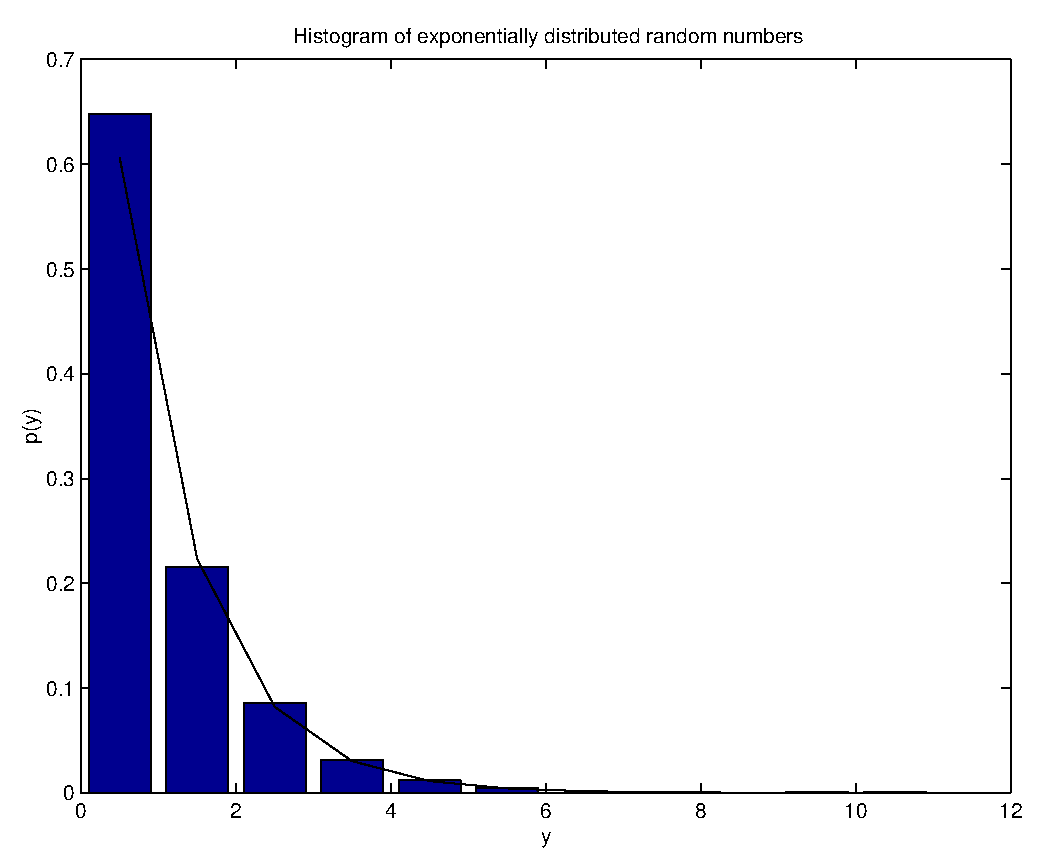
\includegraphics[width=10cm]{./Figures/f_expdistr.eps}
\caption{Histogram of 1000 exponentially distributed random numbers with
mean 1 generated according to the transformation method. The continuous
line represents the expected exponential distribution.}
\end{figure}

\subsection{Gaussian distributed random numbers}
Gaussian distributed random numbers can be obtained with the help 
of the multidimensional random variable transformation theorem.
Let us consider the transformation
\begin{eqnarray}
\label{GAUSS-GEN1}
y_1 & = & \sqrt{-2\log(x_1)} \cos(2 \pi x_2) \\
\label{GAUSS_GEN2}
y_2 & = & \sqrt{-2\log(x_1)} \sin(2 \pi x_2),
\end{eqnarray}
where $X_1$ and $X_2$ are uniformly distributed random numbers on 
the interval $[0,1)$. Equivalently we can write
\begin{eqnarray*}
x_1 & = & \exp[-\frac{1}{2}(y_1^2+y_2^2)] \\
x_2 & = & \frac{1}{2 \pi} \arctan\left( \frac{y_1}{y_2}\right).
\end{eqnarray*}
it is now straightforward  to show that the Jacobian determinant
reads
\begin{equation*}
\frac{\partial(x_1,x_2)}{\partial(y_1,y_2)} = 
   - \left[ \frac{1}{\sqrt{2 \pi}} \exp(-y_1^2/2)\right]
   \left[ \frac{1}{\sqrt{2 \pi}} \exp(-y_2^2/2)\right].
\end{equation*}
The right hand side of the above equation corresponds to the 
product of two independent Gaussian distributions. Thus it follows
from the multidimensional version of the random variable 
transformation  theorem for invertible distributions that the
two random number generated according to Eqs. (\ref{GAUSS-GEN1}) 
and (\ref{GAUSS-GEN2}) are Gaussian distributed. This algorithm 
which allows the generation of two Gaussian random numbers from 
two uniformly distributed ones is called the Box--Muller method.

It is clear that it easy to implement the above algorithm in 
MATLAB. This is done in the program {\sf gaussdistr.m} which generates
gaussian random numbers with mean value $mu$ and variance $sigma$.

\subsubsection{Listing of the program gaussdistr.m}

The corresponding histogram obtained by running the program for
n=1000, mu=0, sigma=2 can be seen in Fig. (\ref{F_GAUSSDISTR}).
\begin{figure}
\label{F_GAUSSDISTR}
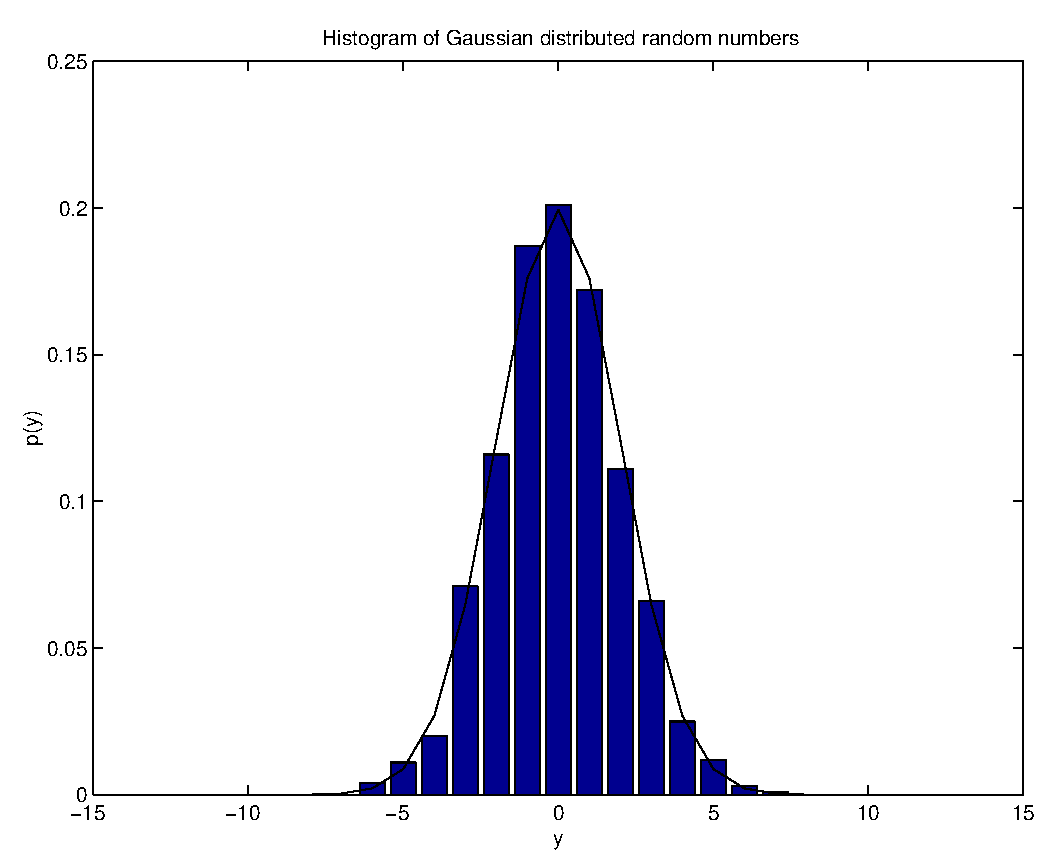
\includegraphics[width=10cm]{./Figures/f_gaussdistr.eps}
\caption{Histogram of 1000 Gaussian distributed random numbers with
mean 0 and variance 2 generated according to the Box-Muller method. 
The continuous line represents the expected Gaussian density.}
\end{figure}

Let us end this subsection by mentioned that normal distributed
random numbers can be generated in MATLAB with the help of 
the function {\sf randn}.

\section{The acceptance--rejection technique}
The acceptance--rejection technique is a method of wide 
applicability. In its original formulation it is due to 
von--Neumann. The basic idea is to sample a random number
from some known and appropriate probability distribution and to 
perform a test to determine whether or not it is acceptable for 
use or not. We follow Rubinstein but consider for simplicity only
the one--dimensional case.

Let us assume that the stochastic variable $X$ is defined on the 
interval $a \le x \le b$ and is distributed according to the
probability density $p(x)$. We write this probability distribution 
as
\begin{equation*}
p(x) = C d(x) q(x),
\end{equation*}
where $C$ is a normalization constant $C \ge 1$, $q(x)$ is also a 
probability distribution and $0 \le d(x) \le 1$. The probability 
distribution $q(x)$ is the importance function, and  we are 
supposed to know how to generate random variates distrubuted 
according to it.

The accepatnce--rejection method works as follows. We generate two
random variates, $\xi$ is uniformly distributed on the interval
$[0,1)$ and $Y$ is distributed according to $q(y)$. Then we test
whether or nor the equality
\begin{equation*}
\xi \le d(y)
\end{equation*}
holds or not. If  the conditione $\xi \le d(y)$ is satisfied, 
then $Y$ is accepted as 
a random variate distributed according to $p(x)$.  If
the condition is not satisfied, the pair $(\xi,y)$ is rejected, 
and we have to try again.

It is easy to demonstrate that the above methd works. Let us apply
Bayes'formula to the conditional probability $p(x|\xi \le d(y)$:
\begin{equation}
\label{A-R-BAYES}
p(x|\xi \le d(y) = \frac{{\rm Prob}(p(x|\xi \le d(y)|Y=x)q(x)}
                  {{\rm Prob}(\xi \le d(y))}.
\end{equation}
It is straightforward to compute
\begin{eqnarray*}
{\rm Prob}(p(x|\xi \le d(y)|Y=x) &=& {\rm Prob}(\xi \le d(x)) = 
          d(x) \\
{\rm Prob}(\xi \le d(y)) & = & \int {\rm Prob}(\xi \le d(Y|Y=x)) q(x) dx \\
               &= & \int q(x) d(x)dx = \int dx \frac{p(x)}{C} = 
                   \frac{1}{C}.
\end{eqnarray*}
Inserting into (\ref{A-R-BAYES}) we obatin finally
\begin{equation*}
p(x|\xi \le d(y) = p(x),
\end{equation*}
which completes the proof.

The above discussion also makes evident the role of the constant
$C$. The efficiency of the method depends on the inequality $\xi \le 
d(y)$, for independent trials the probability of success is given 
by $1/C$. $C$ represents the average number of passes which must 
be made with the algorithm in order to select a variate. It is 
clear, that in order for the method to be efficient it must be 
easy to generate random numbers according to $q(x)$ and the 
efficiency should be large, i.e., $C$ should be close to one.

In the original formulation by von--Neumann the comparison 
function was simply chosen to be the uniform distribution. If
$M$ is the maximum of $p(x)$ then we choose
\begin{eqnarray*}
q(x) & = & \frac{1}{b-a} \\
d(x) & = & \frac{p(x)}{M} \\
C & = & M(b-a).
\end{eqnarray*}
The von--Neumann algorithm then simply reads \\
1. Generate $\chi_1$ and $\chi_2$ uniformly distributed in 
    $[0,1)$. \\
2. Evaluate $Y=a+\chi_2(b-a)$. \\
3. If $\chi_1 \le p(x)/M$ then $Y$ is a variate distributed 
    according to $p(x)$. \\
4. Go to 1.

As a simple example we want to generate random numbers on $[0,1)$    
distributed according to
\begin{equation*}
p(x) = 3x^2; \;\;\; 0 \le x <1.
\end{equation*}
We choose $C=3$ and apply the von--Neumann algorithm. \\
1. Generate $\chi_1$ and $\chi_2$ uniformly distributed in 
    $[0,1)$. \\
2. Test the inequality $\chi_1 \le \chi_2^2.$     \\
3. If the equality holds we accept $\chi_2$ as a random number 
generated according to $p(x)$.

The above algorithm has been implemented in MATLAB in the program
{\sf neumann.m}, which we run for $n=1000$ and $n=5000$. The 
result of the latter run can be seen in Fig. (\ref{F_NEUMANN}).
\begin{figure}
\label{F_NEUMANN}
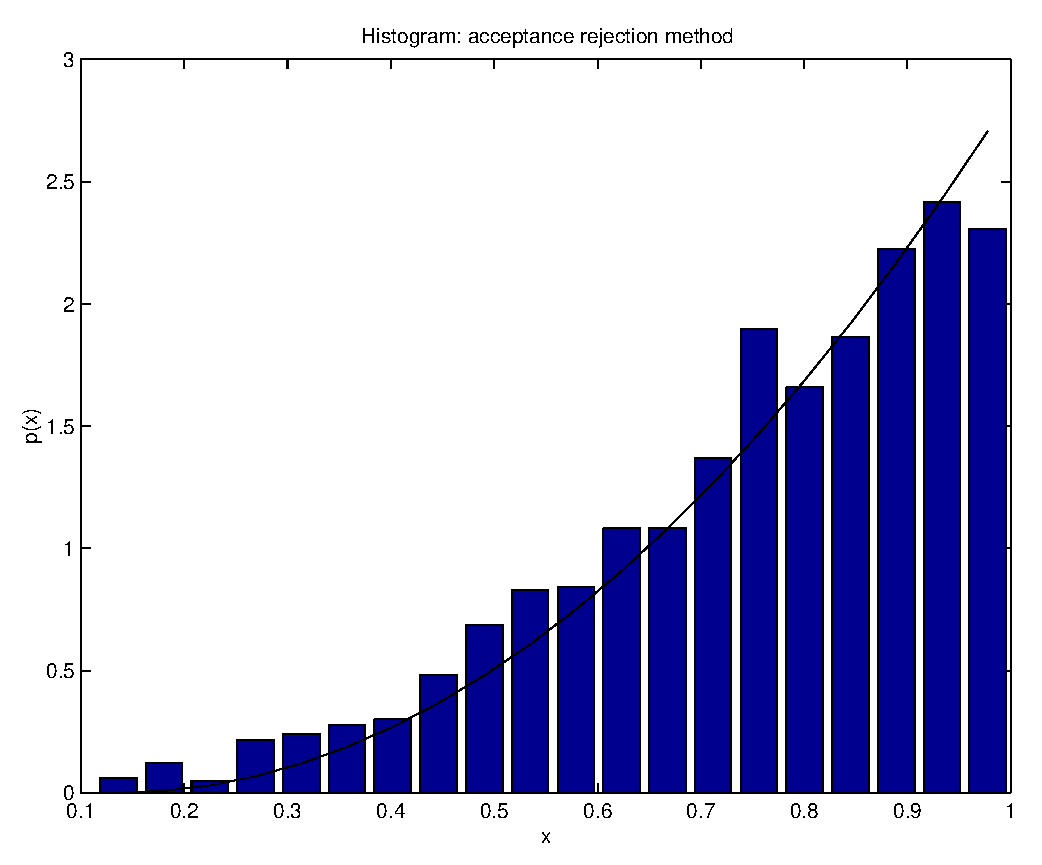
\includegraphics[width=10cm]{./Figures/f_neumann.eps}
\caption{Histogram of 5000 random numbers distributed
according to $p(x) = 3x^2$ generated with the von--Neumann
acceptance--rejection technique.
The continuous line represents the exact density $p(x)$.}
\end{figure}
In the program we count the number of successful trials. The ratio
of successful trials to the total number of drawn random pairs for 
the run shown
is 0.3328, which is in good agreement we the expected theoretical
value of $1/C=1/3$.

\subsubsection{Listing of the program neumann.m}




%\subsection{Poisson distributed random numbers}

\section{Variance reduction: Importance Sampling}
In this section we will see how the Monte--Carlo integration
algorithms can considerably be improved. The importance sampling 
technique will be our first encounter with a so--called variance 
reduction technique. We already know that the estimation of 
integrals by the Monte--Carlo method is affected with errors. The
basic idea of variance reduction techniques is to use known 
informations about the problem in order to improve the efficiency 
of the simulation. Obviuosly, if nothing is known about the 
problem no variance reduction can be achieved. On the other 
extreme, if we have full knowledge the variance will be reduced to 
zero, and there will be no need for a simulation. It is always 
important to be aware of what is known about the system.

We now consider the problem of estimating the integral
\begin{equation}
\label{INT_VARRED}
I = \int dx f(x).
\end{equation}
The central idea of importance sampling is to select random 
variates from regions in proportion to the importance these 
regions make to the integral we want to evaluate, instead of 
spreading them evenly. To this end we rewite the integral 
(\ref{INT_VARRED}) in the form
\begin{equation*}
I = \int \frac{f(x)}{p(x)} p(x) dx = \langle 
\frac{f(x)}{p(x)}\rangle,
\end{equation*}
where $X$ is a random variable with probability density $p(x)$.
$P(x)$ is called the importance sampling distribution.  Since the
integral is obviously the expectation value of the function $f(x)/p(x)$
it can be estimated using $N$ random numbers $X_i$ distributed 
according to $p(x)$
\begin{equation*}
\hat{I}_N = \frac{1}{N} \sum_{i=1}^N \frac{f(x_i)}{p(x_i)}.
\end{equation*}
The function $p(x)$ has to be chosen in such a way that the 
variance of $f(x)/p(x)$ 
\begin{equation*}
{\rm Var} = \langle (\frac{f(x)}{p(x)}-I)^2\rangle
   = \int_a^b \frac{f^2(x)}{p(x)}dx - I^2
\end{equation*}
is minimal. If $f(x)>0$ it follows from the above equation that
${\rm Var}=0$ if we choose $p(x)$ as $p(x) = f(x)/I$. 
Unfortunately, this choice implies that we have to know already 
the integral we want to solve. In general, the variance can 
essentially be reduced if $p(x)$ is chosen to resemble $f(x)$.

As an example we consider the integral
\begin{equation}
\label{I_MCI_IS}
I= \int_0^1 dx \exp(-x^2).
\end{equation}
In the first two columns of table (\ref{T_MCI_IS}) we show
the results of two estimates of the above integral with the 
help of the standard Monte--Carlo integration. In the third column 
we show the results of the importance sampling integration.

\begin{table}\label{T_MCI_IS}
\caption{Monte--Carlo estimates of the integral (\ref{I_MCI_IS})
using the standard method $p(x)=1$ and the importance sampling method
$p(x)=a\exp(-x)$}
\begin{center}
\begin{tabular}{llll}
 ~             & $p(x) =1$ & $p(x) =1$ & $p(x)=a\exp(-x)$ \\ \hline
$N$            & 1000      & 16384      & 1000           \\
$I$            & 0.736087  & 0.74504    & 0.748340        \\
$\sigma_I$     & 0.00131   & 0.000317   & $9.65 \times 10^{-5}$ \\
CPU time/trial (s) & 0.000660  & 0.003837   & 0.000860  \\
total CPU time (s) & 0.66      & 62.86      & 0.86 
\end{tabular}
\end{center}
\end{table}
The simulation was performed with the help of the program
{\sf mciis.m} whose listing can be seen below.

\subsubsection{Listing of the program mciis.m}
%\includelistings{.\Listings\mciis.m}

The importance sampling function is chosen to be $p(x)=a\exp(-x)$,
where the constant $a$ is chosen such that $p(x)$ is normalized
on the  unit interval. Accordingly the $N$ random numbers $X_i$
distributed according to $p(x)$ are generated with the help of the
inversion method. Since
\begin{equation*}
P(x) = \int_0^x dx' p(x') = a[1-\exp(-1)]
\end{equation*}
the exponentially distributed random numbers on the interval $[0,1)$
are generated according to
\begin{equation*}
X = - \log(1- \chi/a),
\end{equation*}
where the $chi$ are uniformly distributed random numbers on the 
interval $[0,1)$. The generation of these random numbers is 
performed in lines x to y.

It is important to remark that although the computation time per
trial is larger in the importance sampling technique the total CPU 
time is smaller compared to the standard Monte Carlo algorithm 
because a much smaller number of realizations is required in order
to achieve a desired accuracy (variance).





\section{Self--Avoiding random walks}
\subsection{Simple sampling}
\subsection{Importance sampling}
%%%%%%%%%%%%%%%%%%%%%%%%%%%%%%%%%%%%%%%%%%%%%%%%%%%%
%%%%%%%%%%%%%%%%%%%%%%%%%%%%%%%%%%%%%%%%%%%%%%%%%%%%%
%%%%%%%%%%%%%%%%%%%%%%%%%%%%%%%%%%%%%%%%%%%%%%%%%%%%%
%%%%%%%%%%%%%%%%%%%%%%%%%%%%%%%%%%%%%%%%%%%%%%%%%%%%%
%%%%%%%%%%%%%%%%%%%%%%%%%%%%%%%%%%%%%%%%%%%%%%%%%%%%%
%%%%%%%%%%%%%%%%%%%%%%%%%%%%%%%%%%%%%%%%%%%%%%%%%%%%%
%%%%%%%%%%%%%%%%%%%%%%%%%%%%%%%%%%%%%%%%%%%%%%%%%%%%%
\chapter{Stochastische Prozesse}
Master-Gleichungen

\chapter{Monte Carlo Methoden in der statistischen Mechanik}
Metropolis; Ising; Finite-Size Effects; Random Walks; SAW (?)
Simulated annealing; travelling salesman;

\chapter{Non-equilibrium MC}
Chemische Reaktionen, Diffusion; Reaktions-Diffusion, Turbulenz.

\chapter{Brownsche Dynamik Simulationen}
Omega-entwicklung; SDE;


\chapter{Rest}
stochastische Resonanzen; Muster Erkennung; random Walks;

\chapter{Stochastische Wellenfunktionsmethoden}


%%% Chapter 4 
\chapter{Markov processes and master equations}
This chapter is devoted
to the introduction of some mathematical concepts, which allow the
correct treatment of time--dependent probabilistic phenomena. 
Such processes occur in many branches of physics. A typical example,
is for instance, the dynamics of the velocity field in a turbulent fluid.
We will introduce stochastic processes as time dependent stochastic 
variables and we will 
learn how the dynamics of a particular class of stochastic 
processes, the so--called Markov processes  is described 
with the help of differential Chapman--Kolmogorov equations. 
These concepts will be applied
in the next chapters to typical examples from statistical physics.

\section{Stochastic processes}
We have already learned in Chap. 2 that once a stochastic variable 
$X$ has been defined it is possible to define other stochastic 
variables, say $Y$, as functions of $X$ by some mapping $f$. In 
particular, the quantity $Y$ may be a function of an additional
time variable $t$, i.e.,
\begin{equation*}
Y(t) = f(X,t).
\end{equation*}
Sloppy speaking, such a quantity $Y(t)$ is called a {\em stochastic
processes}. If we insert for $X$ one of its possible values $x$
we obtain an ordinary function
\begin{equation*}
y(t) = f(x,t),
\end{equation*}
which is a {\em realization} of the stochastic process
\cite{VAN_KAMPEN}. It is 
customary in statistical physics to regard the stochastic process 
as an {\em ensemble} of such realizations.

It follows immediately from the random variable transformation 
theorem that the probability density for $Y(t)$ to take the value
$y$ at time $t$ is given by
\begin{equation*}
P_1(y,t) = \int dx  \delta(y-f(x,t)) P(x)
\end{equation*}
and, accordingly, the joint probability density that $Y$ has the
value $y_1$ at time $t_1$, the value $y_2$ at time $t_2$, 
$\ldots$, and the value $y_n$ at time $t_n$ is given by
\begin{eqnarray*}
\lefteqn{P_n(y_1,t_1;y_2,t_2; \ldots, y_n,t_n)} \\
&& = \int dx \delta(y_1-f(x,t_1))\delta(y_2-f(x,t_2)) \cdots 
   \delta(y_n-f(x,t_n))  P(x).
\end{eqnarray*}
In such a way an infinite hierarchy of joint probability densities
$P_n$ $(n=1,2,\ldots)$ is defined, which allows the evaluation of 
expectation values like
\begin{eqnarray*}
\lefteqn{<Y(t_1) Y(t_2) \cdots Y(t_n)>} \\
&& = \int dy_1 \int dy_2 \cdots \int dy_n 
        y_1 y_2 \cdots y_n P_n(y_1,t_1;y_2,t_2; \ldots, y_n,t_n).
\end{eqnarray*}
It has been shown by Kolmogorov (\cite{VAN_KAMPEN}) that the 
hierarchy of joint probability densities introduced above 
completely specifies
a stochastic process if the following four consistency conditions 
are satisfied \\
(i) $P_n \ge 0$; \\
(ii) $P_n$ is a symmetric function of the pairs $(y_1,t_1)$, 
$\ldots$, $(y_n,t_n)$; \\
(iii) $\int dy_n P_n(y_1,t_1; \ldots , y_n,t_n) =
     P_{n-1}(y_1,t_1; \ldots ; y_{n-1},t_{n-1})$; \\
(iv) $\int dy_1 P(y_1,t_1) =1$.

Thus, the hierarchy of joint probability densities constitutes an 
alternative way to define stochastic processes. 
With increasing $n$ the description of the stochastic process gets
more precise. It is important to 
make the following remarks.  The condition (iii) implies that each 
density $P_n$ includes the knowledge of all previous densities
$P_k$ with $k<n$. Furthermore, the density $P_n$ does have the 
following property if two time arguments are identical
\begin{equation*}
P_n(x,t;y_1,t;y_2,t_2; \ldots ; y_{n-1},t_{n-1}) = 
P_{n-1}(x,t;y_2,t_2; \ldots ; y_{n-1},t_{n-1})
\delta(x-y_1).
\end{equation*}
The hierarchy of probability densities is also the starting point 
for the classification of stochastic processes. A stochastic 
process is said to be purely random if events at different times 
are not correlated. In this case the joint probability density 
factorizes, i.e. we have
\begin{eqnarray*}
P_2(y_1,t_1;y_2,t_2) &=& P_1(y_1,t_1) P_1(y_2,t_2) \\
P_3(y_1,t_1;y_2,t_2;y_3,t_3) &=& P_1(y_1,t_1) P_1(y_2,t_2)P_1(y_3,t_3) 
\\
\text{and so on.} &&
\end{eqnarray*}
This means that the value of $Y$ at time $t$ is completely 
independent of its values in the past and in the future. An even
more special case occurs when the $P_1(y_i,t_i)$ are independent 
of $t_i$. In this case the same probability law governs the 
process for all times. Such processes are called
{\em Bernoulli trials} (\cite{gardiner}). In the next section we 
will introduce the next most simple class, the {\em Markov processes},
in which the knowledge of only the presents determines the future.


\section{Markov processes}
In order to define the class of stochastic processes, which will be 
of central importance in the forthcoming theoretical discussions 
and in the examples of the next chapters, we will formulate
the {\em Markov assumption}. This assumption is formulated in 
terms of conditional probability densities which we 
will denote by
$T_n(x,t|y_1,t_1;y_2,t_2; \ldots, y_n,t_n)$. This quantity gives 
the probability that the stochastic process takes the value $x$ at 
time $t$ given that it had the value $y_1$ at time $t_1$, $y_2$
at time $t_2$, $\ldots$, $y_n$ at time $t_n$, where we assume that
$t_1< \cdots <t_n < t$.  The conditional probability density has 
the following properties \\
(i) $T_n \ge 0$, \\
(ii) $\int dx T_n = 1$,  \\
(iii) $T_n(x,t|y_1,t;y_2,t_2; \ldots, y_n,t_n) = \delta(x-y_1)$.\\
As we already know the joint probability density $P_n$ can be 
expressed with the help of Bayes' theorem through the conditional 
probability density $T_{n-1}$ as
\begin{eqnarray*}
\lefteqn{P_n(x,t;y_1,t_1;y_2,t_2; \ldots, y_{n-1},t_{n-1})} \\
&& = P_{n-1}(y_1,t_1;y_2,t_2; \ldots, y_{n-1},t_{n-1})
T_{n-1}(x,t|y_1,t_1;y_2,t_2; \ldots, y_{n-1},t_{n-1}).
\end{eqnarray*}
Now we are in the position to define the class of Markov 
processes. Let $t_1< \cdots <t_n < t_{n+1}$ be an ordered sequence 
of times. A Markov process is defined through the following 
condition for the conditional probability density of the
stochastic process
\begin{equation*}
T_{n}(y_{n+1},t_{n+1}|y_1,t;y_2,t_2; \ldots, y_{n},t_{n})
= T_{1}(y_{n+1},t_{n+1}|y_{n},t_{n}).
\end{equation*}
In other words, the conditional probability density at $t_{n+1}$
given the value of $y_n$ at time $t_n$ is uniquely determined and 
is not affected by any value of $y$ at earlier times. Thus, the
conditional probability density is determined completely by the 
knowledge of the most recent condition.
The above definition implies that for a Markov process all
$T_n$ with $n \ge 1$ can be determined from the
conditional probability density $T_1$, which will also be called
the one step 
transition probability density. As an immediate consequence a Markov 
processes is completely characterized by the knowledge of the
one step transition probability and by the probability density
$P_1$. With the help of these two functions we can reconstruct the 
whole hierarchy of probability densities. For example, we
have
\begin{eqnarray}
\label{P3}
P_3(y_1,t_1;y_2,t_2;y_3,t_3) &=& 
      P_2(y_1,t_1;y_2,t_2) T_2(y_3,t_3|y_1,t_1;y_2,t_2)   
         \nonumber \\
    & = & T_1(y_3,t_3|y_2,t_2) T_1(y_2,t_2|y_1,t_1)
           P_1(y_1,t_1).
\end{eqnarray}
Integrating the above equation (\ref{P3}) over $y_2$ we obtain 
\begin{equation}
P_2(y_1,t_1;y_3,t_3) = P_1(y_1,t_1) 
       \int dy_2 T_1(y_3,t_3|y_2,t_2) T_1(y_2,t_2|y_1,t_1).
\end{equation}
Dividing both sides by $P_1(y_1,t_1)$ we obtain an identity which 
must be obeyed by the transition probability of any Markov process
\begin{equation}
\label{CHAPMAN_KOLMOGOROV}
T_1(y_3,t_3|y_1,t_1) =  
       \int dy_2 T_1(y_3,t_3|y_2,t_2) T_1(y_2,t_2|y_1,t_1).
\end{equation}
The above identity is called the {\em Chapman--Komogorov 
equation}. It has a simple interpretation. The transition 
probability between two states $y_1$ and $y_3$ with $t_1 <t_3$
corresponds to the product of the transition probability between 
the initial state and some intermediate state and the transition 
between this intermediate state and the final state integrated
over all intermediate states.

As we already noted the functions $P_1$ and $T_1$ uniquely define 
a Markov process. However, these two functions are not arbitrary.
They must satisfy the Chapman--Kolmogorov equation and the obvious
consistency condition
\begin{equation}
\label{CONSISTENCY}
P_1(y_2,t_2) =  
       \int dy_1  T_1(y_2,t_2|y_1,t_1) P_1(y_1,t_1).
\end{equation}
For the sake of a compact notation we will write now $P=P_1$ and 
$T=T_1$.


\section{The differential Chapman--Kolmogorov equation}
We now derive a differential  form of the Chapman--Kolmogorov 
equation which is more practical for physical applications.
We will proceed in two steps. First, we introduce the concept
of generator of a stochastic process. Second, we will construct
with the help of the generator an equation of motion for the
transition probabilty density.

\subsection{The generator of a Markov process}
We consider the time evolution of the expectation value
of  a function $f(y)$.
Thus,
\begin{eqnarray*}
\frac{\partial}{\partial t} \langle f(y) \rangle &=&
 \frac{\partial}{\partial t} 
    \left\{  \int dy f(y) P(y,t)  \right\}  \\
 &= & \lim_{\Delta t \rightarrow 0} \frac{1}{\Delta t}
       \left\{  \int dy f(y) \left[P(y,t+\Delta t) - P(y,t) \right]  
       \right\}.
\end{eqnarray*}
Making use of the consistency condition (\ref{CONSISTENCY}) 
in the first term 
on the right--hand side of the above equation we obtain
\begin{equation*}
\frac{\partial}{\partial t} \langle f(y) \rangle =
   \lim_{\Delta t \rightarrow 0} \frac{1}{\Delta t}
    \left\{  \int dy \int dy' f(y) T(y,t+\Delta t|y',t) P(y',t) 
         - \int dy f(y) P(y,t) 
       \right\}.
\end{equation*}
We rename the integration variables in the positive 
term of the right--hand side of the above equation ($y \rightarrow y'$,
$y' \rightarrow y$) to obtain
\begin{equation*}
\frac{\partial}{\partial t} \langle f(y) \rangle =
   \lim_{\Delta t \rightarrow 0} \frac{1}{\Delta t}
    \left\{  \int dy  \int dy' \left[ f(y') T(y',t+\Delta t|y,t) 
         - \delta(y-y') f(y') \right] P(y,t) 
       \right\},
\end{equation*}
which we can also write as
\begin{equation*}
\frac{\partial}{\partial t} \langle f(y) \rangle =
\int dy P(y,t) \lim_{\Delta t \rightarrow 0} \frac{1}{\Delta t}
\left\{ \int dy' \left[ f(y') T(y',t+\Delta t|y,t) 
         - \delta(y-y') f(y') \right].
\right\}
\end{equation*}
At this point it is convenient to introduce the infinitesimal 
generator of a Markov process ${\cal{A}}$ as
\begin{equation}
\label{DEF_GENERATOR}
{\cal{A}}(t) f(x) = \lim_{\Delta t \rightarrow 0}
    \frac{1}{\Delta t} 
    \left[\int dy f(y)T(y,t+\Delta t|x,t) - f(x)  \right].
\end{equation}
$f(y)$ is some measurable function for which the above 
limit exists. Evidently ${\cal{A}}$ is a linear operator, which 
can be determined from the transition probability density. 
When the operator ${\cal{A}}$ operates on $f$ it describes the
change of the expectation value of $f$ in an infinitesimal time 
step. As a consequence of the Chapman--Kolmogorov equation each time 
step $t-t_1$ can be decomposed into a sequence of smaller time 
steps. So it is plausible to characterize the Markov
process by regarding infinitesimal time steps. 
The importance of the generator ${\cal{A}}$ lies in the fact
that together with some initial condition $P(x,t=0)$ it specifies
uniquely the Markov process.
The time evolution equation for the expectation value can be written 
in the compact and suggestive form
\begin{equation}
\label{EQ_EXPECTATION}
\frac{\partial}{\partial t} \langle f \rangle = 
\langle {\cal{A}} f \rangle.
\end{equation}


\subsection{The differential Chapman--Kolmogorov equation}
With the help of the generator we derive an equation of motion for
the transition probability $T$.
Multiplying equation (\ref{DEF_GENERATOR}) 
with $T(x,t|x',t')$ ($t'<t$) and 
integrating over $x$ we obtain
\begin{eqnarray*}
\lefteqn{\int dx \left[ {\cal{A}}(t) f(x) \right] T(x,t|x',t')} \\
&& = \lim_{\Delta t \rightarrow 0}
    \frac{1}{\Delta t} 
    \left[\int dy f(y)T(y,t+\Delta t|x',t') - 
        \int dx f(x) T(x,t|x',t')  \right],
\end{eqnarray*}
where we made use of the Chapman--Kolmogorov equation.
We now rename the variable $y$ on the right--hand side of the above 
equation and call it $x$ and perform the limit $\Delta t \rightarrow 
0$
\begin{equation}
\label{KOL_FORWARD_0}
\int dx \left[ {\cal{A}}(t) f(x) \right] T(x,t|x',t') =
  \int dx f(x) \frac{\partial}{\partial t} T(x,t|x',t').
\end{equation}
It is convenient to introduce the adjoint operator ${\cal{A}}^{\dagger}$
to the generator ${\cal{A}}$ according to the following definition
\begin{equation}
\label{ADJOINT}
\int dx \left[ {\cal{A}}(t) f(x) \right] T(x,t|x',t') \equiv
\int dx f(x) \left[ {\cal{A}}^{\dagger}(t)  T(x,t|x',t') \right].
\end{equation}
We will see in the next sections how the adjoint operator is
explicitely constructed.
Inserting Eq. (\ref{ADJOINT}) into Eq. (\ref{KOL_FORWARD_0})
and considering that (\ref{ADJOINT}) holds for any 
function $f(x)$ we conclude that the equation of motion for the 
transition probability is given by
\begin{equation}
\label{KOL_FORWARD}
\frac{\partial}{\partial t} T(x,t|x',t') =
{\cal{A}}^{\dagger}(t) T(x,t|x',t').
\end{equation}
We will call the above equation the {\em differential 
Chapman--Kolmogorov equation}. The differential 
Chapman--Kolmogorov equation is the central equation of this 
chapter. Together with some initial probability distribution it 
defines completely a Markov process. With its help it is possible
to compute time--dependent expectation values and multi--time 
correlation functions. Because of its importance, it is sometimes
named the {\em master equation} in the physical literature.


Let us end this subsection with an overview of this chapter. In Fig. 
(\ref{F_CHAP$_OVERVIEW}) we have schematically summerized the theory
of stochastic processes.  Particular emphasis is given to Markov
processes
which will be at the center of the present and of the next chapters.
In the next section we will construct
the differential Chapman--Komogorov equation for deterministic Markov 
processes, for jump processes and for diffusion processes.
\begin{figure}
\label{F_CHAP$_OVERVIEW}
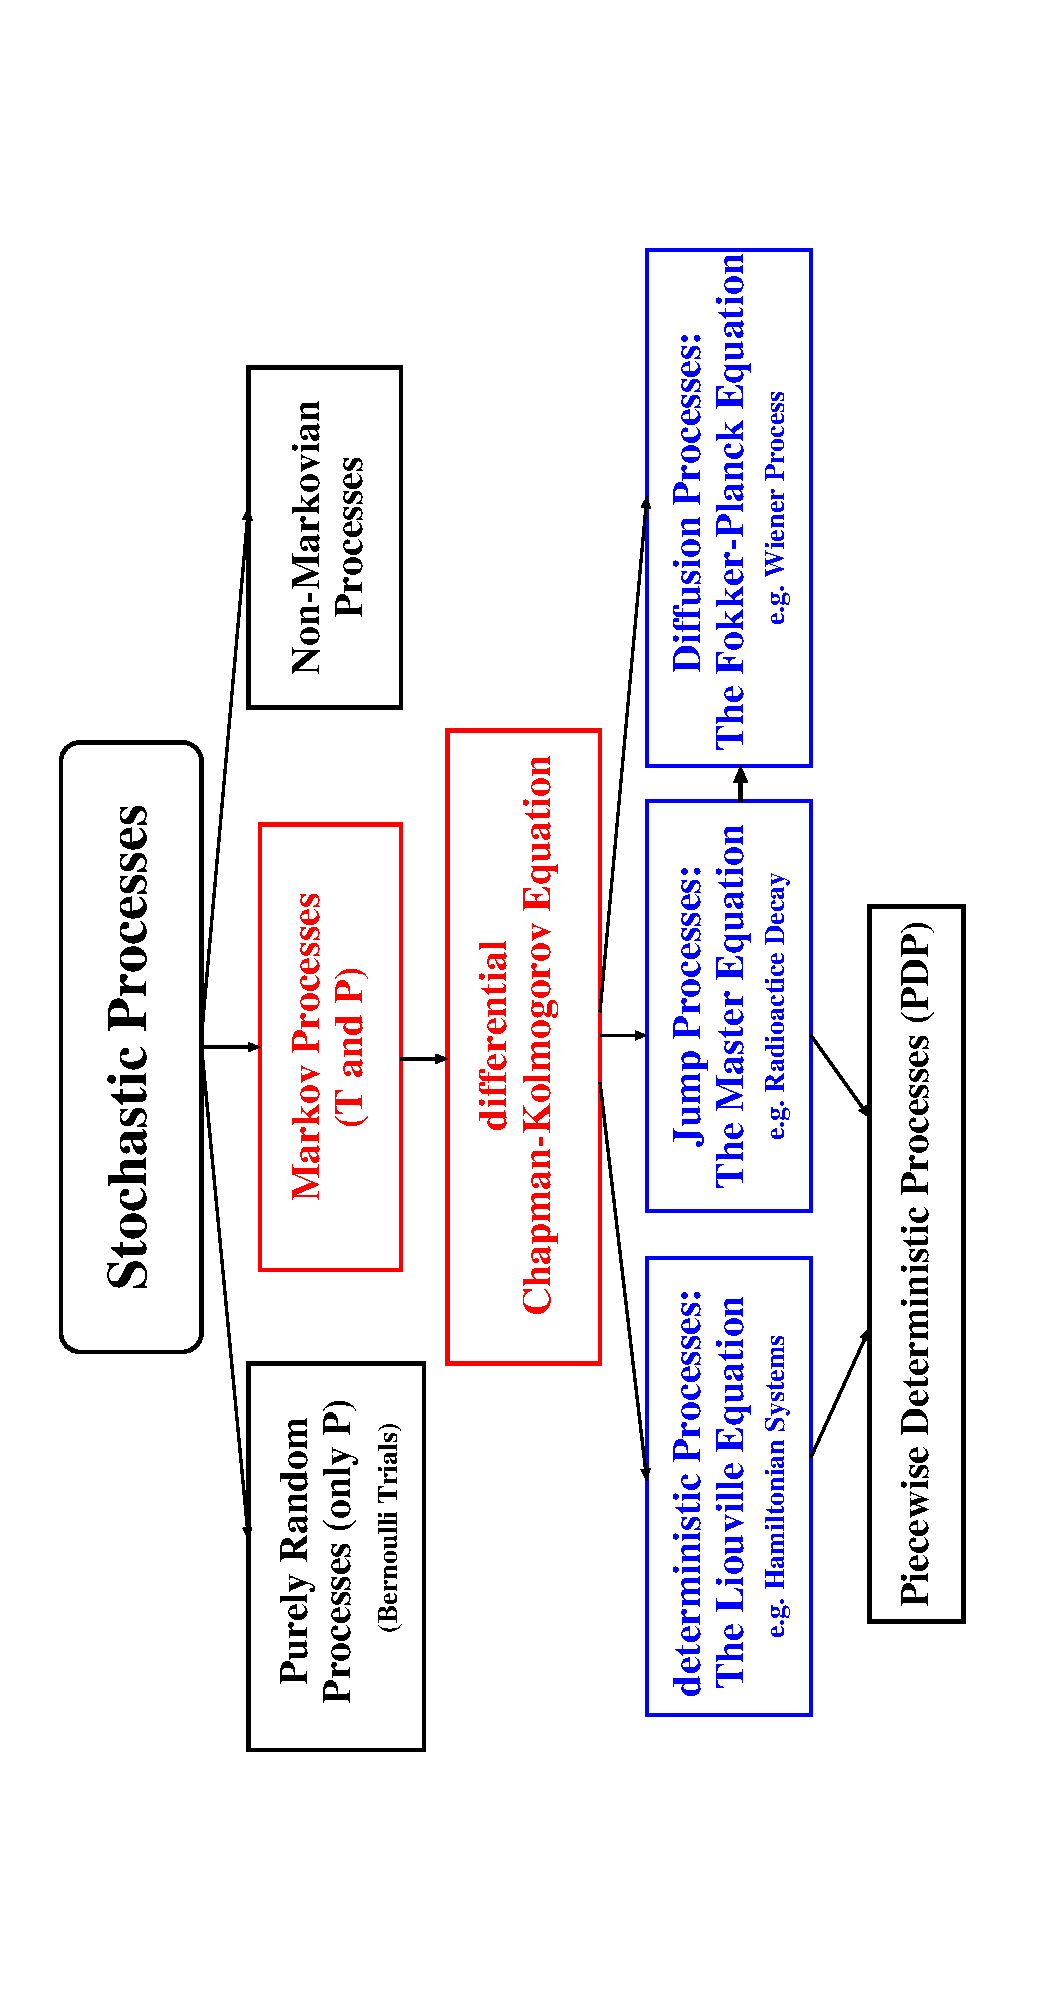
\includegraphics[width=10cm]{./Figures/f_chap4_overview.eps}
\caption{Overview of the theor of stochastic processes.}
\end{figure}

\section{The Liouville equation}
Let us consider a physical system whose dynamics is described
by a system of ordinary differential equations of first order
\begin{equation}
\label{ORDINARY_DIFF}
\frac{d}{dt} x(t) = g(x(t)),
\end{equation}
where $g$ is a function $R^d \rightarrow R^d$. 
It is clear that Hamiltonian systems belong to this class 
(\cite{ARNOLD}). The initial 
condition is
\begin{equation*}
x(0) = x \in R^d.
\end{equation*}
We denote the unique solution of this equation by $\phi(t,x)$,
where the $x$ stresses the dependence on the initial condition.

If $f:R^d \rightarrow R^d$ is a continuous differentiable function
then it follows from Eq. (\ref{ORDINARY_DIFF}) 
\begin{equation}\label{COORDINATE_FREE}
\frac{d}{dt} f(x(t)) = \sum_i \frac{\partial f}{\partial x_i}
          (x(t)) g^i(x(t)),
\end{equation}
where $g^i$ denotes the $i$--th component of $g$. 


With the help of these formal preliminaries it is easy to 
construct the generator of a deterministic Markov process.
Obviously we have for the expectation value
\begin{equation*}
Ef(x(t)) = f(\phi(x,t)),
\end{equation*}
where the symbol $E$ denotes the expectation value.

Inserting the above expectation value into the definition of a 
generator (\ref{DEF_GENERATOR}) we immediately obtain
\begin{eqnarray*}
{\cal{A}}_L(t) f & = & \lim_{t\rightarrow 0} \frac{1}{t}
                        \left[ Ef(x(t)) - f(x)\right] \\
             & = & \lim_{t\rightarrow 0} \frac{1}{t}
                        \left[ f(\phi(x,t)) - f(\phi(0,x))\right] \\
              & = & \frac{d}{dt} f(x) ,
\end{eqnarray*}
and finally, using Eq. (\ref{COORDINATE_FREE}),
\begin{equation*}
{\cal{A}}_L(t) f = \sum_i \frac{\partial f}{\partial x_i}(x) g^i(x).
\end{equation*}


Having determined the generator it is now straightforward to 
evaluate the corresponding differential Chapman--Kolmogorov 
equation. To this end we only 
have to determine the operator which is adjoint to
${\cal{A}}_L$ by partial integration. It is evident that we have
\begin{eqnarray}
\label{GEN_DET0}
\int dx \left[{\cal{A}}_L f(x) \right]h(x) &=&
          \sum_i \int dx \left[g^i 
           \frac{\partial f}{\partial x_i} \right] h(x) \nonumber \\
     & = & -\sum_i f \frac{\partial}{\partial x_i} g^i h(x).      
\end{eqnarray}
Since Eq. (\ref{GEN_DET0}) holds for any function $h(x)$
\begin{equation}
\label{GEN_DET_A}
{\cal{A}}_L^{\dagger} h(x) = -\sum_i \frac{\partial}{\partial x_i}
    \left(g_i h(x) \right).
\end{equation}
Inserting (\ref{GEN_DET_A}) into the differential Chapman--Kolmogorov 
equation
(\ref{KOL_FORWARD}) 
leads to the master equation for a deterministic Markov process
\begin{equation}
\frac{\partial}{\partial t} T(x,t|x',t') =
 - \sum_i \frac{\partial}{\partial x_i}
     \left(g_i(x)T(x,t|x',t')  \right).
\end{equation}
In statistical physics the above equation is called the Liouville 
equation.
 
The Liouville equation is the starting point for the microscopic 
description of matter for classical as well as for quantum 
mechanical systems. It is one of the fundamental equations of 
statistical physics. 

\subsection{Example: Classical statistical mechanics}
In order to give an example of the occurrence
of the Liouville equation we consider a closed classical system
with $N$ degrees of freedom, e.g., $N$ particles in a 
three--dimensional box. We know from classical mechanics, that the 
state  of such a system is completely specified by the set of $6N$
independent variables $\vec{p}^N=(\vec{p}_1, \ldots, \vec{p}_N)$ 
and $\vec{q}^N=(\vec{q}_1, \ldots, \vec{q}_N)$, where $\vec{p}_i$
and $\vec{q}_i$ denote the momentum and the position of the 
$i$--th particle. 

If the system is Hamiltonian (\cite{ARNOLD}), 
i.e., if we can define a Hamiltonian
$H(\vec{p}^N,\vec{q}^N)$, then the time evolution of the momentum 
and of the position of the particles is given by Hamilton's 
equations of motion
\begin{eqnarray*}
\frac{d}{dt} \vec{p}_i &=& - \frac{\partial H}{\partial \vec{q}_i} 
             \\
\frac{d}{dt} \vec{q}_i &=&  \frac{\partial H}{\partial \vec{p}_i} 
.
\end{eqnarray*}

In a real physical system it is not possible to specify exactly 
the state of the system. There is always some uncertainty in the 
initial conditions. Therefore, we regard $(\vec{p}^N,\vec{q}^N)$
as a stochastic variable which is initially distributed according 
to the joint probability density $P^N(\vec{p}^N,\vec{q}^N,0)$. 
The dynamics of this probability distribution
is described by the following 
Liouville equation
\begin{equation*}
\frac{\partial}{\partial t} P^N =  {\cal{A}}_L^{\dagger} P^N,
\end{equation*}
where
\begin{equation*}
{\cal{A}}_L^{\dagger} = -\sum_{i=1}^N \left( 
      \frac{\partial H}{\partial \vec{p}_i} 
            \cdot \frac{\partial}{\partial \vec{q}_i} 
         - \frac{\partial H}{\partial \vec{q}_i} 
             \cdot \frac{\partial}{\partial \vec{p}_i}.
      \right)
\end{equation*}
The Liouville equation is often written in the following form
\begin{equation*}
i \frac{\partial}{\partial t} P^N(\vec{p}^N,\vec{q}^N,t) =  
  {\cal{L}} P^N(\vec{p}^N,\vec{q}^N,t),
\end{equation*}
where
\begin{equation*}
{\cal{L}} =  i {\cal{A}}_L^{\dagger}.
\end{equation*}
The operator ${\cal{L}}$ is called the Liouville operator.
If the probability disribution at time $t=0$ is known the above 
Liouville equation may be integrated formally  
to find the probability density
at later times $t$
\begin{equation*}
P^N(\vec{p}^N,\vec{q}^N,t) = \exp(-i {\cal{L}}t)  
P^N(\vec{p}^N,\vec{q}^N,0).
\end{equation*}
The Liouville equation is the starting point for the evaluation of 
probability distributions in statistical mechanics. Extensive use 
of the Liouville equation is done in kinetic theory. From the 
Liouville equation it is possible to derive a hierarchy of 
equations for probability densities, the so--called 
BBGKY--hierarchy from which kinetic equations may be derived
(\cite{REICHL}).


\section{The master equation}
Let us now introduce jump processes (\cite{DAVIES,FELLER}).
We consider a system in a given state $x$.  
In order to characterize a jump process, i.e., a process
in which the system undergoes sudden discontinuous changes of its state,
we have to specify the probability for 
the system to remain in $x$ during the time interval $dt$ 
\begin{equation*}
(1-\lambda(x) dt)
\end{equation*}
and the probability that the system jumps from state $x$ to state
$x'$ during the time interval $dt$ 
\begin{equation*}
\lambda(x) Q(x',x) dt,
\end{equation*}
where
\begin{equation}
\label{NORM_Q}
\int dx' Q(x',x) =1.
\end{equation}
Then,
\begin{equation*}
Ef(x(dt+t)) = (1-\lambda(x)dt) f(x)
   + \lambda(x) dt \int dx'f(x') Q(x',x).
\end{equation*}
From the definition of the generator we obtain immediately the
generator of the jump process
\begin{equation}
\label{GEN_JUMP}
{\cal{A}}_M f(x) = \lambda(x) \int dx' \left( f(x') 
-f(x)\right)Q(x',x),
\end{equation}
where we made use of Eq. (\ref{NORM_Q}).
Again, in order to derive the Kolmogorov forward equation we have 
to construct the adjoint operator to ${\cal{A}}_M$.
We start from Eq. (\ref{KOL_FORWARD_0})  
\begin{equation}
\label{KOL_FORWARD_J0}
\int dx \left[ {\cal{A}}_M(t) f(x) \right] T(x,t|x',t') =
  \int dx f(x) \frac{\partial}{\partial t} T(x,t|x',t').
\end{equation}
and insert the generator (\ref{GEN_JUMP}) into the left--hand side 
of the above equation
\begin{eqnarray*}
\lefteqn{\int dx \left[ {\cal{A}}_M(t) f(x) \right] T(x,t|x',t')} 
\\
&=& \int dx \left[ \lambda(x)
       \int dx'' \left(f(x'') -f(x) \right) Q(x'',x) \right] T(x,t|x',t') 
       \\
& = & \int dx \int dx'' \lambda(x) f(x'') Q(x'',x) T(x,t|x',t') \\
& & - \int dx \int dx'' \lambda(x) f(x) Q(x'',x) T(x,t|x',t').
\end{eqnarray*}
By renaming $x \rightarrow x''$ and $x'' \rightarrow x$  in the first line of the
above equation we get
\begin{eqnarray}
\label{ADJOINT_JUMP}
\lefteqn{\int dx  f(x) \int dx'' \lambda(x'')  Q(x,x'') T(x'',t|x',t')}
     \nonumber \\
& & - \int dx f(x) \int dx'' \lambda(x)  Q(x'',x) T(x,t|x',t') \nonumber \\
& \equiv & \int dx f(x) \left[ {\cal{A}}_M^{\dagger}(x) 
          T(x,t|x',t')      \right]
\end{eqnarray}
From Eq. (\ref{KOL_FORWARD_J0}) and from Eq. (\ref{ADJOINT_JUMP}) 
we conclude that the differential Chapman--Kolmogorov equation 
of a jump process
reads
\begin{eqnarray} 
\label{KOL_FORWARD_J1}
\lefteqn{\frac{\partial}{\partial t} T(x,t|x',t') =} \nonumber \\ 
&& \int dx'' \lambda(x'') Q(x,x'') T(x'',t|x',t')
 - \int dx'' \lambda(x) Q(x'',x) T(x,t|x',t').
\end{eqnarray}
Because of Eq. (\ref{NORM_Q}) we can write the above equation also 
in the form
\begin{eqnarray} 
\label{KOL_FORWARD_J2}
\lefteqn{\frac{\partial}{\partial t} T(x,t|x',t') =} \nonumber \\ 
&& \int dx'' \lambda(x'') Q(x,x'') T(x'',t|x',t')
 - \lambda(x) T(x,t|x',t').
\end{eqnarray}
Usually the differential Chapman--Kolmogorov equation for a jump process is 
written in a more suggestive form. To this end we introduce the 
total transition rate pro time unit for a transition from state $x'$ 
into  state $x$ to occur
\begin{equation*}
w(x,x') = \lambda(x') Q(x,x')
\end{equation*}
and write the differential Chapman--Kolmogorov equation 
for a jump process in its final form
\begin{equation}
\label{MASTER_JUMP}
\frac{\partial}{\partial t} T(x,t|x',t') =
 \int dx'' \left( w(x,x'') T(x'',t|x',t')
 - w(x'',x) T(x,t|x',t') \right).
\end{equation}
The above equation is called the master equation. 
The name master equation appears for the first time in a paper by
Nordsieck, Lamb and Uhlenbeck (\cite{NORDSIECK}). 
It was chosen to denote an equation from which
all relevant equations and results can be derived. 

In the physical literature Eq. (\ref{MASTER_JUMP}) is written in 
the simplified form
\begin{equation}
\label{MASTER_JUMP_P}
\frac{\partial}{\partial t} P(x,t) =
 \int dx'' \left( w(x,x'') P(x'',t)
 - w(x'',x) P(x,t) \right).
\end{equation}
This equation has the following meaning (\cite{VAN_KAMPEN}). Take a 
time $t'$ and a state $x'$ and consider 
the solution of Eq. (\ref{MASTER_JUMP_P})
for $t \ge t'$ with the initial condition $P(x,t') = 
\delta(x-x')$. This solution is the conditional transition 
probability $T(x,t|x',t')$ of the Markov process for each choice
of $x'$ and $t'$. It is important to keep in mind that 
Eq. (\ref{MASTER_JUMP_P})
is always to be interpreted as an equation for $T$ and not for 
$P$.

In the above form the physical meaning of the master equation is 
also evident. The master equation is a balance equation for the
probability to find the system in some state. The first term in 
the master equation describes the gain of state due to transitions 
from the other states. The second term is the loss due to the 
transitions from the given state into the others. Evidently,
the term with $x=x'$ does not contribute to the integral.

If the state space of the stochastic process is discrete, i.e.
all integer numbers $n$,
the master equation for the time evolution of $P(n,t)$ will assume 
the following discrete form
\begin{equation}
\label{MASTER_JUMP_P_N}
\frac{\partial}{\partial t} P(n,t) =
 \sum_{n'} \left( w(n,n') P(n')
 - w(n',n) P(n,t) \right).
\end{equation}
We will discuss in the next section how the stochastic processes 
defined in terms of a master equation can be simulated 
numerically.


\section{Stochastic simulation}
In principle there are two ways to treat numerically
stochastic processes which are defined in terms of master
equations. In the first approach one solves numerically the
master equation as a differential equation for the probability
density. Although this deterministic method is direct we will not consider it 
here for the following reason. It  turns out that the direct 
numerical solution of the master equation is not particularly 
efficient from a computational point of view. The second approach,
which we will introduce in this section relies upon the simulation 
of the underlying stochastic process. In other words one considers 
a particle and lets it jump from one state to another with certain 
given transition rates. Such a procedure is called the generation 
of a realization of the stochastic process. If a sufficiently 
great number of realizations has been generated the interesting 
statistical quantities can be evaluated as ensemble averages.

In fact the numerical performance of the direct approach gets 
worse compared to the stochastic simulation with increasing 
dimension of the system considered. We already met a similar 
situation, when we considered numerical algorithms for the 
computation of integrals. There the direct integration of 
multidimensional integrals turned out to be less efficient than 
the Monte--Carlo integration.

In order to formulate a stochastic simulation algorithm we 
consider for simplicity the master equation of a one--step 
process. Sometimes such processes are also called birth--and--death
processes. The range of such processes consists of all integers
$n$ and the matrix of the transition probabilities per unit time
allows only jumps between adjacent sites
\begin{equation*}
w(n',n) \neq 0 \;\;\; \text{for} \;\;\; n'=n \pm 1
\end{equation*}
and
\begin{equation*}
w(n',n) = 0 \;\;\; \text{otherwise}.
\end{equation*}
Exploiting the above structure we can write the master equation 
for the discrete one--dimensional process (\ref{MASTER_JUMP_P_N})
\begin{eqnarray*}
\dot{P}(n,t) &=& w(n,n+1)P(n+1,t) + w(n,n-1)P(n-1,t) \\
       && -w(n+1,n)P(n,t) -w(n-1,n)P(n).
\end{eqnarray*}
Now it is convenient to introduce the following notation
\begin{eqnarray*}
r(n+1) \equiv w(n,n+1) \\
g(n-1) \equiv w(n,n-1),
\end{eqnarray*}
so that the master equation for a general one--step process 
may be written in the following 
suggestive form
\begin{equation}
\label{MASTER_ONE_STEP}
\dot{P}(n,t) = r(n+1)P(n+1,t) + g(n-1)P(n-1,t)
        -[r(n)+ g(n)]P(n,t).
\end{equation}

Let us now assume that at time $t$ the particle is in state
$n$. The total transition rate to leave this state, i.e. to jump 
out of this state either to state $n+1$ or to state $n-1$, is 
given by
\begin{equation}
\label{TOTAL_RATE_ONE_JUMP}
\lambda(n) = r(n) + g(n).
\end{equation}
As we already know  the quantity $\lambda(n) dt$ is the 
probability that the next jump occurs within the infinitesimal 
time step $dt$. Accordingly the probability that the next jump 
occurs after $(N+1)$ time steps $dt$ is given by
\begin{equation*}
q=[1-\lambda(n)dt]^N \lambda(n)dt,
\end{equation*}
where $[1-\lambda(n)dt]^N$ denotes the probability that no jump
occurs during the first $N$ steps. We now write $(N+1)dt =t$, so 
that we have
\begin{equation*}
q= \left( 1 - \frac{\lambda(n) t}{N+1}\right)^N \lambda(n) dt.
\end{equation*}
We now perform the limit $dt \rightarrow 0$ for fixed $t$. This 
limit implies, of course, $N \rightarrow \infty$ and hence the 
probability that a jump occurs after time $t$ is given by
\begin{equation*}
q= \lambda \exp(-\lambda t) dt = f(t) dt.
\end{equation*}
The waiting time distribution for the time of the next jump is an
exponential distribution.
It is now clear what we have to do in order to determine the time 
of the next jump in the stochastic simulation.  
We simply have to draw random times $\tau$, 
which are distributed according to the density $f(t)$. Since $f(t)$
is an exponential distribution, these random times can easily be 
drawn with the help of the inversion method
\begin{equation}
\label{TAU_ONE_STEP}
\tau = - \frac{1}{\lambda(n)} \log(\xi),
\end{equation}
where $\xi$ is a uniformly distributed random number on the 
interval $[0,1)$. 

Having determined the stochastic time of the
next jump we still have to decide which transition actually takes 
place. We have only two possibilities: In case of a jump the 
particle can reach the state $(n-1)$ with probability
\begin{equation*}
y_1 = \frac{r(n)}{\lambda(n)}
\end{equation*}
or the state  $(n+1)$ with probability
\begin{equation}
y_2 = 1 -y_1 = \frac{g(n)}{\lambda(n)}.
\end{equation}
Thus, the algorithm for the simulation of a one--step--process
reads: \\

(i) Draw a uniformly distributed random number $\xi_1$ on $[0,1)$
   and compute the random jump time $\tau$ according to 
   (\ref{TAU_ONE_STEP}). 
   
(ii) Draw a uniformly distributed random number $\xi_2$ on 
$[0,1)$. If the condition $(\xi_2 < y_1)$ is satisfied we set 
$\nu =+1$.  Otherwise we set $\nu =-1$.

(iii) Advance the process
\begin{eqnarray*}
t &\longrightarrow& t+\tau \\
n & \longrightarrow & n + \nu.
\end{eqnarray*}

The flow chart of the algorithm can be seen in Fig. 
(\ref{F_ONESTEP_ALGORITHM}).
\begin{figure}
\label{F_ONESTEP_ALGORITHM}
\includegraphics[width=7cm]{./Figures/f_onestep_algorithm.eps}
\caption{Flow chart of a stochastic simulation of a 
    one--step process. The symbols used
     are explained in the text.}
\end{figure}
The algorithm has been implemented in the program {\texttt{onestep.m}}
whose listing can be seen below. The program {\texttt{onestep.m}} makes
use of a function called {\texttt{decayymaster.m}} in which the
transitions rates $g(n)$ and $r(n)$ are specified. In the 
following subsection we will discuss three typical one--step 
processes. The specific form of the function \texttt{decaymaster} 
will be given there.

\subsubsection{Listing of the program {\texttt{onestep.m}}}
\inputlisting{./Listings/onestep.m}

The program will be applied in the next subsections.


\subsection{Radioactive decay}
As a first example we consider the master equation 
description of the radioactive decay. To this end let
$P(n,t)$ be the probability density to find $n$ radioactive nuclei
at time $t$. The probability for a nucleus to decay in unit time will
be denoted by $\gamma$. The radioactive decay is a typical example
of a one--step process. It is defined through
the transition rates
$g(n) \equiv 0$ and $r(n)= \gamma n$, where $\gamma$ is the decay constant.
Substitution of the above $g(n)$ and $r(n)$ into the master equation
for the one--step process
(\ref{MASTER_ONE_STEP}) yields the master equation of the radioactive 
decay
\begin{equation}
\frac{\partial}{\partial t} P(n,t) = 
\gamma (n+1) P(n+1,t) - \gamma n P(n,t).
\end{equation}
Before we apply the stochastic simulation algorithm to the 
generation of trajectories of the stochastic process we consider
for one moment the above master equation.

The above equation has to be solved for the initial condition
$P(n,0)= \delta(n,n_0)$. 
It is interesting to establish the
relation between the master equation and the macroscopic 
description in terms of differential equations we already met in 
the introduction.
To this end we consider
\begin{eqnarray*}
\sum_{n=0}^{\infty} n \dot{P}(n,t) &=&
       \gamma \sum_{n=0}^{\infty} n(n+1)P(n+1) 
         - \gamma  \sum_{n=0}^{\infty} n^2 P(n) \\
  &=& \gamma \sum_{n=0}^{\infty} (n-1)n P(n) 
         - \gamma  \sum_{n=0}^{\infty} n^2 P(n) \\
  & = & - \gamma \sum_{n=0}^{\infty} n P(n) .
\end{eqnarray*}
Thus we have found the following dynamical equation for the 
average of the stochastic 
variable $N(t)$
\begin{equation}
\frac{d}{dt} \langle N(t) \rangle = - \gamma \langle N(t) \rangle.
\end{equation}
Note that the mean value of the stochastic process obeys the 
differential equation for the concentration. It is clear that the 
above equation has the following solution for the initial value
$\langle N(0)\rangle = n_0$
\begin{equation*}
\langle N(t) \rangle = n_0 \exp(-\gamma t).
\end{equation*}

Let us now turn to the stochastic simulation. In order to use
the program \texttt{onestep.m} we still have to specify
the function \texttt{decaymaster.m}. The listing of this
function can be seen below.
\subsubsection{Listing of the function {\texttt{decaymaster.m}}}
\inputlisting{./Listings/decaymaster.m}

Now we are in the position to simulate the stochastic process of
radioactive decay. We run the program for the following parameters
\texttt{n0=500}, \texttt{tend=30}, and \texttt{nreal=10}.
The decay rate is $\gamma=0.1$.
The result of the simulation can be seen in Fig. (\ref{F_OS_DECAY}).

\begin{figure}
\label{F_OS_DECAY}
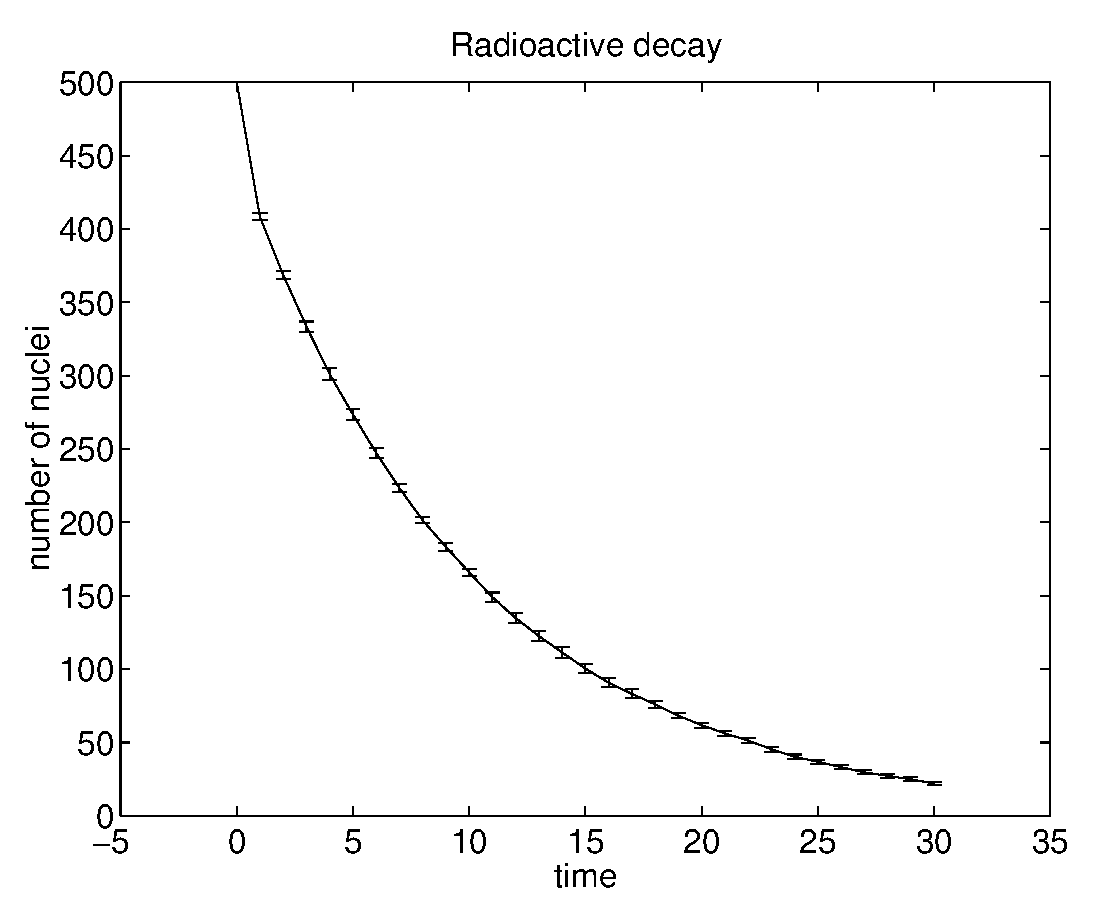
\includegraphics[width=10cm]{./Figures/f_os_decay.eps}
\caption{Stochastic simulation of radioactive decay. The initial
  number of decaying nuclei is {\texttt n0}$= 100$. {\texttt tend}
is 30 and the ensemble average was taken over 10 realizations.
The decay rate is $\gamma=0.1$.}
\end{figure}  

\subsection{The Poisson process}
A further important one--step process is the Poisson process, which
is defined by
\begin{equation}
r(n) = 0; \;\;\; g(n) = q = \text{const}.
\end{equation}
Inserting the above transition rates into the master equation
(\ref{MASTER_ONE_STEP}) we get the master equation defining
the Poisson process
\begin{equation}
\label{MASTER_POISSON}
\frac{\partial}{\partial t} P(n,t|n',t') =
  q [ P(n-1,t|n',t') - P(n,t|n',t')].
\end{equation}
The Poisson process describes a random walk over the integers
$0,1,2,\ldots$. The steps of the walk are all of length $l$ and are 
only to the right. They are performed at random times with 
probability per unit time equal to $q$.

It is instructive to consider the analytical solution of the 
above master equation (\ref{MASTER_POISSON}). The analytical
solution will be constructive with the help of a very useful 
technique which is based upon the characteristic function
\begin{equation*}
G(s,t) = \langle \exp(ins)\rangle = \sum_n P(n,t|n',t') \exp(ins).
\end{equation*}
The  equation of motion for the characteristic function is easily 
obtained with the help of (\ref{MASTER_POISSON}). We find
\begin{equation*}
\frac{\partial}{\partial t} G(s,t) = 
       q \left[ \exp(is) -1 \right] G(s,t).
\end{equation*}
Assuming that at time $t'$ the one--sided random walk starts at
$n'=0$, the initial condition of the above differential equation
reads
\begin{equation*}
G(s,0) = 1.
\end{equation*}
In this case the solution of the above differential equation of 
motion  for the characteristic function is easily found. It reads
\begin{equation*}
G(s,t) = \exp\left\{ tq \left[ \exp(is)-1 \right]\right\}.
\end{equation*}
To read out the analytical solution for the transition probability
$P(n,t|0,0)$ it is convenient to write the above solution in the
form
\begin{eqnarray*}
G(s,t) &= & \exp(-tq) \exp \left[ tq \exp(is)\right] \\
       &= & \sum_{n=0}^{\infty} \exp(-tq) 
             \frac{[tq\exp(is)]^n}{n!}.
\end{eqnarray*}
For $s=0$ and from the definition of the characteristic function
it follows immediately that
\begin{equation*}
P(n,t|0,0) = \exp(-tq) \frac{(tq)^n}{n!},
\end{equation*}
which evidently is a Poisson distribution. As we know the 
characteristic function allows the determination of all moments of 
the stochastic process through the relation
\begin{equation*}
\langle n^m(t) \rangle = \left. 
       \left( -i \frac{\partial}{\partial s} \right) G(s,t)  
       \right|_{s=0}.
\end{equation*}
Applying the above formula we find
\begin{equation*}
\langle n(t) \rangle = qt
\end{equation*}
and
\begin{equation*}
\langle n^2(t) \rangle = qt + (qt)^2.
\end{equation*}
Accordingly, the variance of the Poisson process is given by
\begin{equation*}
\text{Var}(n) = \langle n^2(t) \rangle - \langle n(t) \rangle^2 = 
   qt.
\end{equation*}
The simulation of the Poisson process is straightforward. We make 
use of the program \texttt{onestep.m} and simply write a new 
function \texttt{poissonmaster.m} according to the 
master equation (\ref{MASTER_POISSON}) whose listing can be
seen below.

\subsubsection{Listing of the function {\texttt{poissonmaster.m}}}
\inputlisting{./Listings/poissonmaster.m}

To begin we generate one realization of the Poisson process. To 
this end we run the program with the following parameters:
\texttt{nstart=0}, \texttt{tend=30}, \texttt{nreal=1}. In the 
function \texttt{poissonmaster} we have chosen the transition rate
to be \texttt{q=1}. One realization of the Poisson process can be
seen in Fig. (\ref{F_OS_POI_R}).
\begin{figure}
\label{F_OS_POI_R}
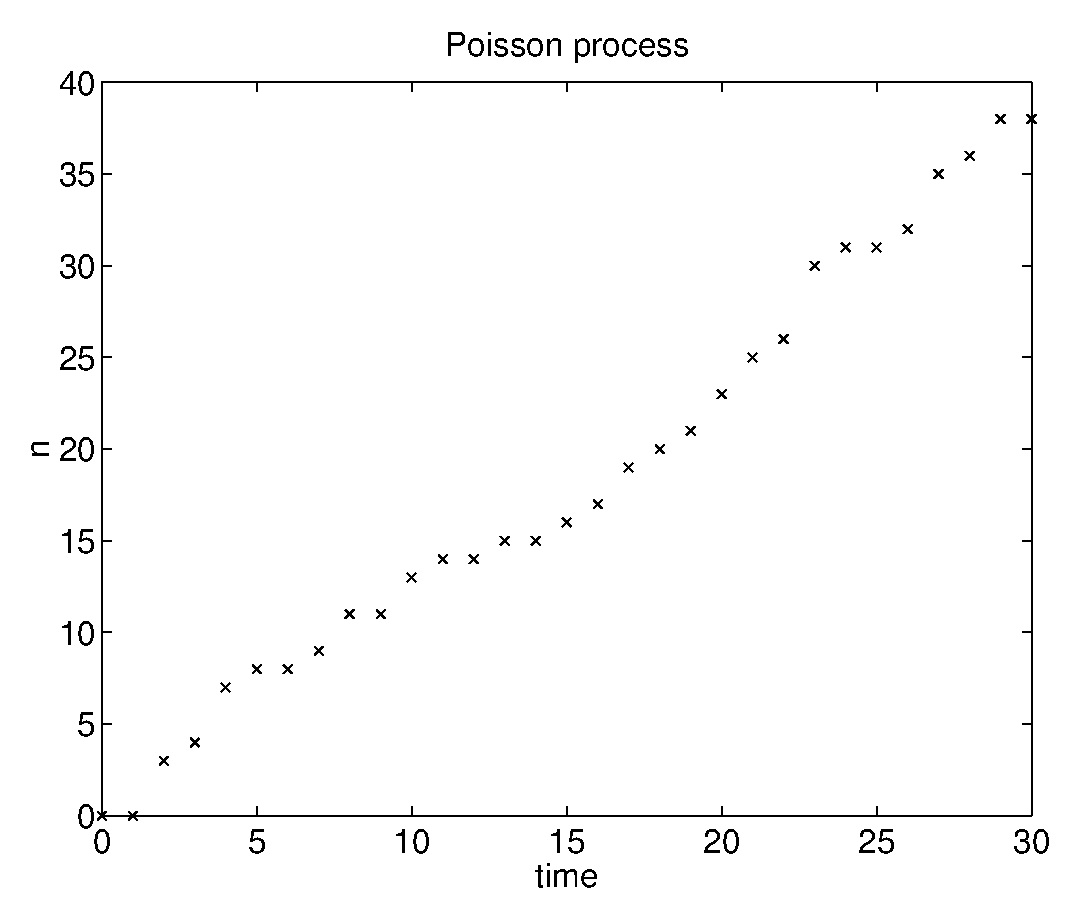
\includegraphics[width=10cm]{./Figures/f_os_poi_r.eps}
\caption{Stochastic simulation of the Poisson process. The 
one--sided random walk starts at \texttt{nstart=0}.  
{\texttt tend} is 30 and \texttt{nreal=1}.
The jump rate is \texttt{q=1}.}
\end{figure}  
In Fig. (\ref{F_OS_POI_1}) we show an ensemble average over 20
realizations of the Poisson process. The other parameters are 
unchanged.
\begin{figure}
\label{F_OS_POI_1}
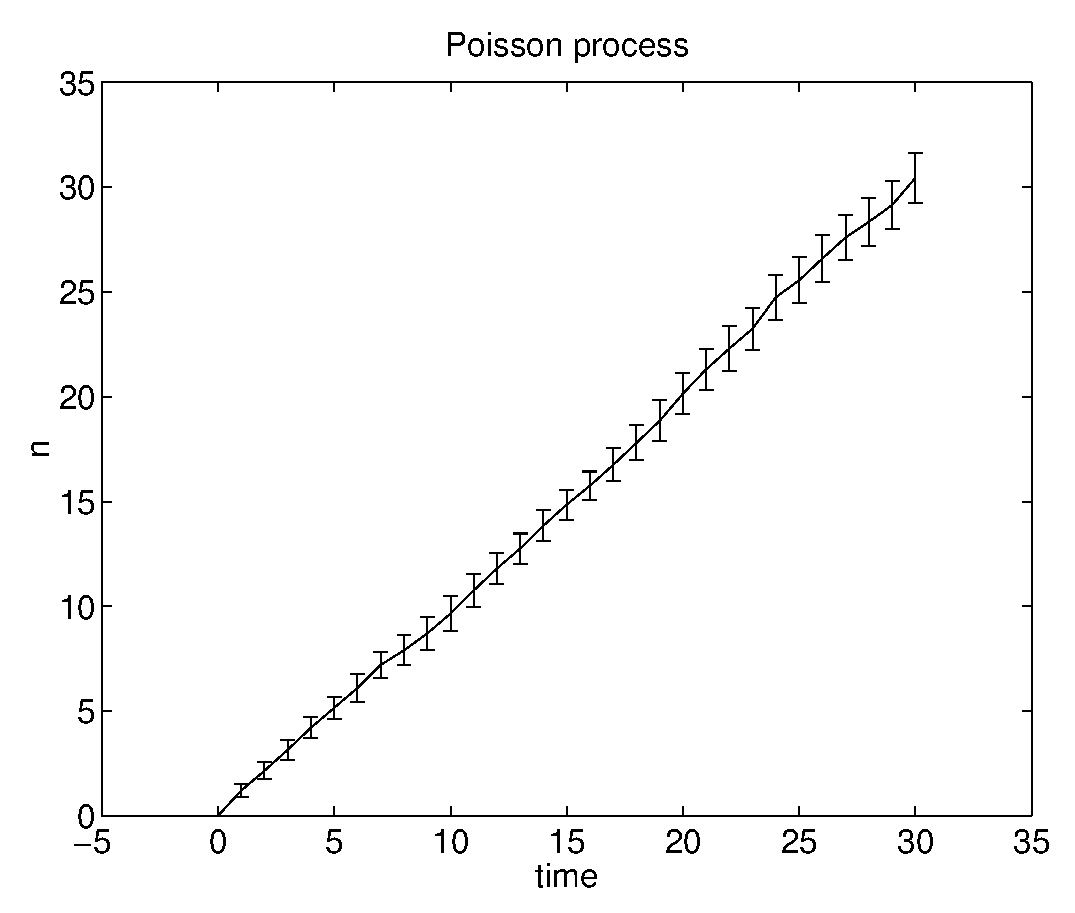
\includegraphics[width=10cm]{./Figures/f_os_poi_1.eps}
\caption{Stochastic simulation of the Poisson process. The 
one--sided random walk starts at \texttt{nstart=0}.  
{\texttt tend} is 30 and \texttt{nreal=20}.
The jump rate is \texttt{q=1}.}
\end{figure}
It is interesting to consider the limit of continuous space for the
Poisson process. Let us denote the distance travelled by 
\begin{equation*}
x=nl.
\end{equation*}
As a function of the new stochastic variable $x$ the 
characteristic function $\tilde{G}$ is
\begin{equation*}
\tilde{G}(s,t) = \langle \exp(isx) \rangle = 
     \exp\{tq[\exp(ils)-1] \}.
\end{equation*}
We perform the limit $l \longrightarrow 0$ keeping 
\begin{equation*}
ql=v=\text{const}
\end{equation*}
and obtain keeping only the terms linear in $l$ in the Taylor
expansion of $\exp(ils)$
\begin{equation*}
\lim_{l\rightarrow 0}\tilde{G}(s,t) = \exp(itvs).
\end{equation*}
So, in the continuum limit the transition probability is
\begin{equation*}
P(x,t|0,0) = \delta(x-vt).
\end{equation*}
Thus, the Poisson process has a deterministic limit. This can also 
be seen by considering, that in the same limit the master equation
for the Poisson process turns into the Liouville equation
\begin{equation*}
\frac{\partial}{\partial t} P(x,t|0,0) = -v 
\frac{\partial}{\partial x} P(x,t|0,0),
\end{equation*}
whose solution is the deterministic process we have just derived.
This behaviour can also be seen in the simulation. To this end
we run the program \texttt{onestep} with the function 
\texttt{poissonmaster} choosing \texttt{q=10}. The result of the 
simulation can be seen in Fig. (\ref{F_OS_POI_2}).
\begin{figure}
\label{F_OS_POI_2}
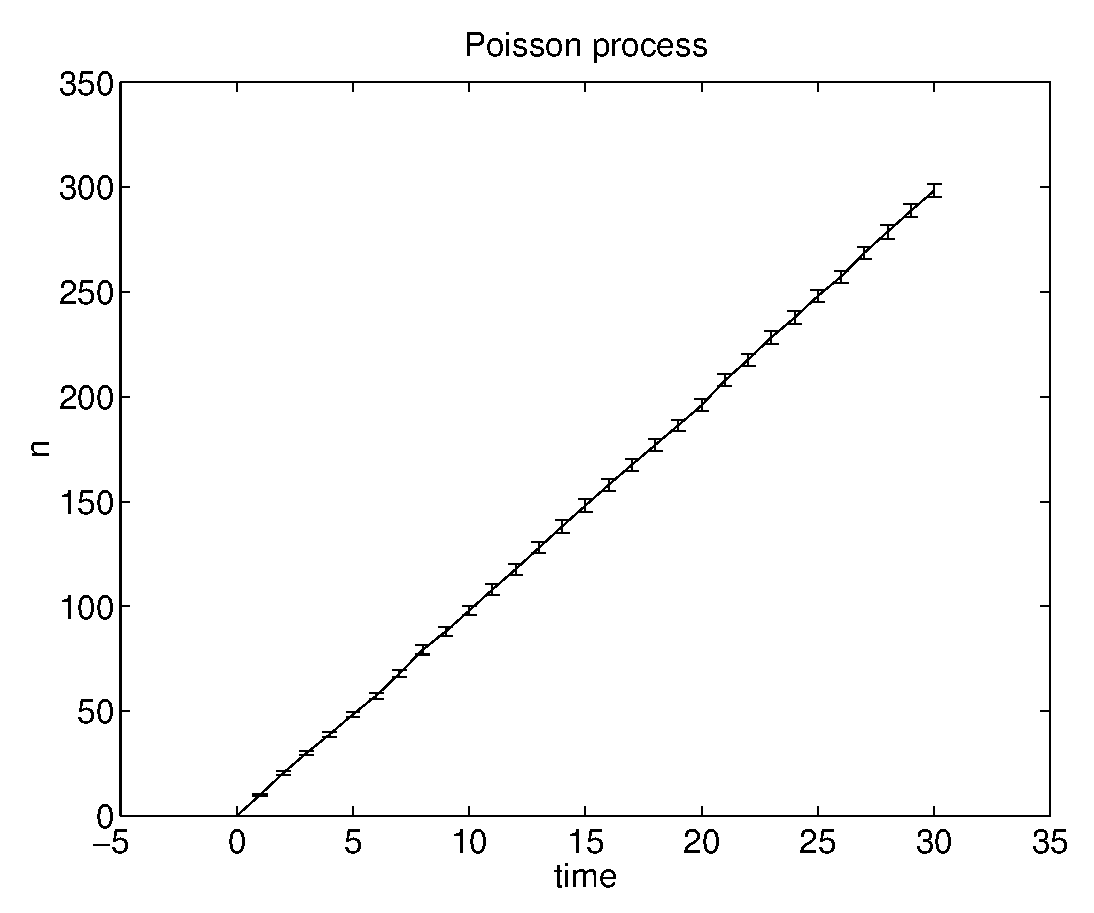
\includegraphics[width=10cm]{./Figures/f_os_poi_2.eps}
\caption{Stochastic simulation of the Poisson process. The 
one--sided random walk starts at \texttt{nstart=0}.  
{\texttt tend} is 30 and \texttt{nreal=20}.
The jump rate is \texttt{q=10}.}
\end{figure}
As we can see for a larger value of \texttt{q} the variance of the
process gets smaller. Thus the dynamics of the process is nearly 
deterministic.

\subsection{The continuous time random walk}
In this subsection we want to consider the master equation for
the one--dimensional random walk. The steps of the walker are of 
length $l$. The positions of the walker are $nl$ and are labelled
by the integer $n$. We already considered the random walk problem 
in Chapter 2.  There the walker was allowed to take steps 
to the left and to the right at some 
discrete times $N\tau$, where the time step $\tau$ was fixed.
Now, we consider a random walk which is continuous in time. The 
walker is allowed to take steps to the left or to the right with 
the probability per unit time $q$. This process is again described 
by a master equation for a one--step process (\ref{MASTER_ONE_STEP})
by choosing
\begin{equation*}
r(n) =g(n) =q.
\end{equation*}
Thus the master equation for the continuous time random walk
reads
\begin{eqnarray}
\label{MASTERWALK}
\frac{\partial}{\partial t} P(n,t|n',t') &=& 
       q \left\{ P(n+1,t|n',t') + P(n-1,t|n',t')\right. \\
       && \left.  - 2 P(n,t|n',t')  \right\}. \nonumber
\end{eqnarray}
Again the above master equation is easily solved with the help of 
the characteristic function $G(s,t)$. It is easy to check that the
characteristic function satisfies the equation
\begin{equation*}
\frac{\partial}{\partial t} G(s,t) = q [\exp(is) +\exp(-is) -2] G(s,t).
\end{equation*}
Assuming that the walker starts at time $t'=0$ in $n'=0$ we find
$G(s,0)=1$ and the solution of the above equation reads
\begin{equation*}
G(s,t) = \exp\{[ \exp(is) +\exp(-is) -2  ]tq\}.
\end{equation*}
With the help of the above expression for the characteristic 
function the moments are easily evaluated. We find
\begin{eqnarray*}
\langle n(t) \rangle &=& 0, \\
\langle n^2(t) \rangle &=& 2tq.
\end{eqnarray*}
Again we find the typical behaviour of a diffusive process.

The continuous time random walk is also easily simulated with the
help of the program \texttt{onestep}. To this end we have to write
a new function \texttt{walkmaster.m} which implements the 
appropriate transition rates.

\subsubsection{Listing of the function \texttt{walkmaster.m}}
\inputlisting{./Listings/walkmaster.m}

We run the program with the following parameters: 
\texttt{nstart=0}, \texttt{nreal=10}, \texttt{tend=30}, and
\texttt{q=1}. The result of the simulation can be seen in
Fig. (\ref{F_CTRW}).
\begin{figure}
\label{F_CTRW}
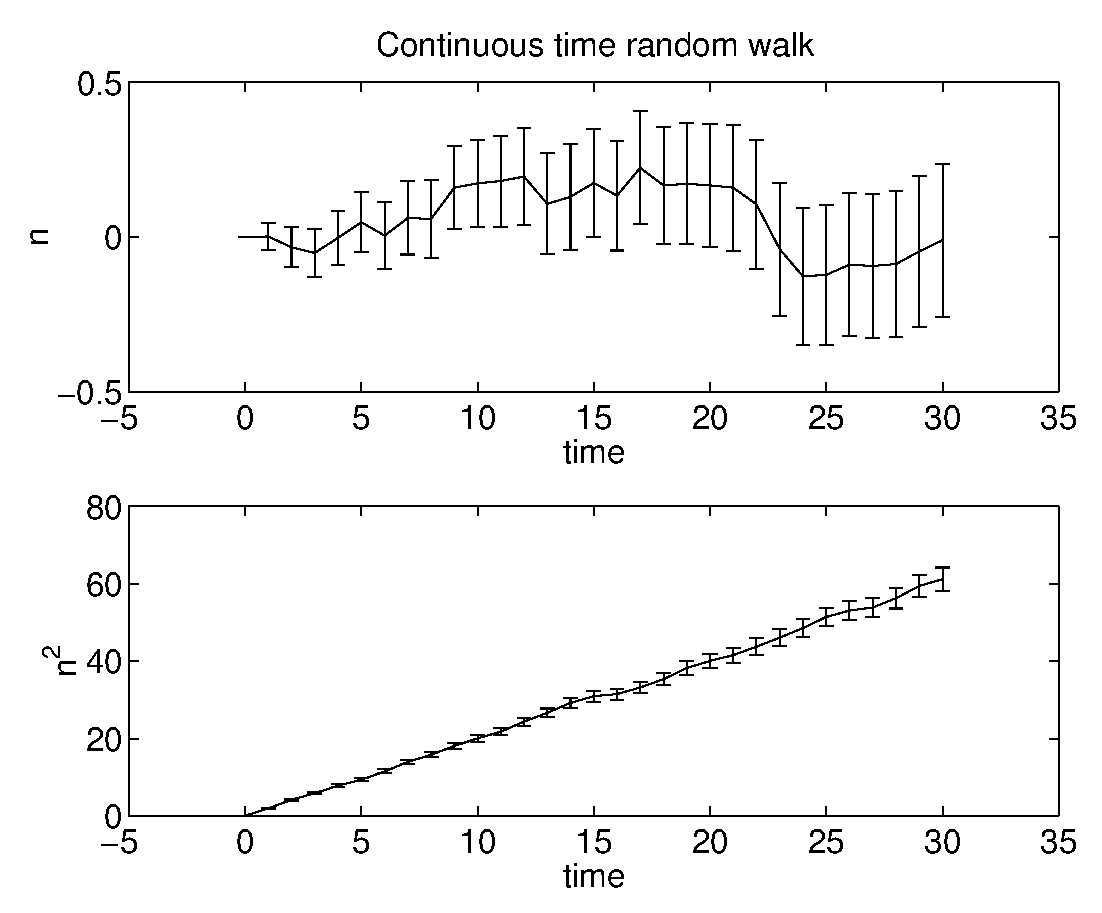
\includegraphics[width=10cm]{./Figures/f_ctrw.eps}
\caption{Stochastic simulation of the continuous time
random walk. The 
random walk starts at \texttt{nstart=0}.  
{\texttt tend} is 30 and \texttt{nreal=20}.
The jump rate is \texttt{q=1}.}
\end{figure}

It is of particular interest to look at the continuous space limit
of the continuous time random walk. Again we write for the 
distance travelled by the walker $x=nl$. The characteristic
function as a function of $x$ reads
\begin{eqnarray*}
\tilde{G}(s,t) &=& G(sl,t) = \langle \exp(ixs) \rangle \\
                &=& \exp\{[\exp(ils) + \exp(-ils)-2]tq \}.
\end{eqnarray*}
The limit of infinitesimally small steps $l \longrightarrow 0$ 
leads to
\begin{equation}
\label{CHAR_WALK_X}
\tilde{G}(s,t) = \exp(-s^2tD),
\end{equation}
where
\begin{equation*}
D=\lim_{l\rightarrow 0} (l^2q).
\end{equation*}
The quantity $D$ can be interpreted as the mean square distance 
traveled  per unit time.  The characteristic function (\ref{CHAR_WALK_X})
is the characteristic function of a Gaussian process of the form
\begin{equation*}
P(x,t|0,0) = \frac{1}{(4\pi Dt)^{1/2}} \exp\left( -x^2/4Dt 
\right).
\end{equation*}
This is the transition probability of a so--called {\em Wiener process},
which can be regarded as a continuous time random walk in the 
limit of infinitesimally small step size. We will consider the 
Wiener process in more detail in the next section.

The following remark may serve as an introduction to the next 
section. Of course, we can also expand directly the master equation
(\ref{MASTERWALK}) as a function of $x$ up to second order terms 
in $l$ and get
\begin{equation*}
\frac{\partial}{\partial t} P(x,t|0,0) =
     (l^2q) \frac{\partial^2}{\partial x^2} P(x,t|0,0),
\end{equation*}
which is a special type of Fokker--Planck equation, as we will see 
in the next section.

\section{The Fokker--Planck equation}
In this section we want to derive the Fokker--Planck equation
(\cite{RISKEN}),
which is a special type of master equation (\cite{VAN_KAMPEN})
in the limit of small jumps.
We begin by expressing the transition probability $w$ as a 
function of the size $r$ of the jump and of the starting point
\begin{equation*}
w(y,y') = w(y';r); \;\;\; r=y-y'.
\end{equation*}
The master equation (\ref{MASTER_JUMP_P}) then reads
\begin{equation}
\label{MASTER_SMALL_JUMP}
\frac{\partial}{\partial t} P(y,t) =
  \int dr w(y-r;r)P(y-r,t) - \int dr w(y;-r)P(y,t).
\end{equation}
In order to consider the limit of small jumps essentially
two assumptions will be needed. The first is that
the function
$w(y;r)$ will be a sharply peaked function of $r$ and will
vary slowly with $y$. To be more precise we assume that a $\delta >0$
exists such that
\begin{eqnarray*}
w(y';r)  & \approx & 0 \;\;\; \text{for} \;\;\; |r|> \delta \\
w(y'+\Delta y;r) & \approx & w(y';r) \;\;\; \text{for} \;\;\; |\Delta y| < 
\delta.
\end{eqnarray*}
The second assumption is that the solution $P(y,t)$ of the master equation 
in this limit will be a slowly varying function of $y$.

If these assumptions hold it is safe to expand the shift from $y$
to $y-r$ in the first integral in 
Eq. (\ref{MASTER_SMALL_JUMP}) in a Taylor series
\begin{equation}
\label{MASTER_EXPAND}
\frac{\partial}{\partial t} P(y,t) = \sum_{\nu=0}^{\infty}
   \frac{(-1)^{\nu}}{\nu!} \left( \frac{\partial}{\partial y} 
   \right)^{\nu}
    \left\{  a_{\nu}(y) P(y,t) \right\}
    - P(y,t) \int_{-\infty}^{\infty} dr w(y;-r),
\end{equation}
where we have defined
\begin{equation*}
a_{\nu}(y) = \int_{-\infty}^{\infty} dr r^{\nu} w(y;r).
\end{equation*}
Since the zeroth term in the sum and the second term of 
Eq. (\ref{MASTER_EXPAND}) cancel the small jumps expansion 
of the master equation reads
\begin{equation}
\frac{\partial}{\partial t} P(y,t) = \sum_{\nu=1}^{\infty}
   \frac{(-1)^{\nu}}{\nu!} \left( \frac{\partial}{\partial y} 
   \right)^{\nu}
    \left\{  a_{\nu}(y) P(y,t) \right\}.
\end{equation}
The above expansion is called the Kramers--Moyal expansion. 
Formally, we can write
\begin{equation}
\frac{\partial}{\partial t} P(y,t) = {\cal{A}}_{KM}^{\dagger}(y)
         P(y,t),
\end{equation}
where we introduced the adjoint generator
\begin{equation*}
{\cal{A}}_{KM}^{\dagger}(y) = \sum_{\nu=1}^{\infty}
   \frac{(-1)^{\nu}}{\nu!} \left( \frac{\partial}{\partial y} 
   \right)^{\nu}
     a_{\nu}(y).
\end{equation*}
It is easy to show by partial integration that the corresponding
generator  reads
\begin{equation*}
{\cal{A}}_{KM}(y) = \sum_{\nu=1}^{\infty}
   \frac{1}{\nu!}  a_{\nu}(y)
    \left( \frac{\partial}{\partial y} 
   \right)^{\nu}.
\end{equation*}
It is clear that dealing with the {\em Kramers--Moyal} expansion will 
not be easier than dealing with the original master equation.

A particularly interesting and useful approximation to a jump process is 
obtained by keeping only terms up to the second order in $\nu$
\begin{equation}
\label{FOKKER_PLANCK}
\frac{\partial}{\partial t} P(y,t) =
-\frac{\partial}{\partial y} \left\{ a_1(y) P(y,t) \right\}
   + \frac{1}{2} \frac{\partial^2}{\partial y^2} 
      \left\{ a_2(y) P(y,t) \right\}.
\end{equation}
The above equation is called the {\em Fokker--Planck equation}.
The first term on the right--hand side is usually called the drift
term since it is essentially Liouvillian. The second term
on the right--hand side is the diffusion term. In a later section
we will learn how to deal with this equation.

\subsection{The Wiener process}
Let us consider the important special case 
of vanishing drift, i.e. $a_1=0$, and diffusion coefficient
equal to one, i.e. $a_2=1$. The generator takes the form 
\begin{equation}
\label{WIENER_GENERATOR}
{\cal{A}}_W = {\cal{A}}_W^{\dagger} = \frac{1}{2} 
     \frac{\partial^2}{\partial y^2},
\end{equation}
and it defines a Wiener process. We already met the corresponding
Fokker--Planck equation, 
when we considered the continuous space limit of the the 
continuous time random walk.
Now we want to write down this Fokker--Planck equation in the form
\begin{equation*}
\frac{\partial}{\partial t}T(w,t|w_0,t_0) =
  \frac{1}{2} \frac{\partial^2}{\partial x^2} T(w,t|w_0,t_0).
\end{equation*}
The above equation can easily be solved with the help of the 
characteristic function
\begin{equation*}
G(s,t) = \int dw T(w,t|w_0,t_0) \exp(isw),
\end{equation*}
where we have assumed that the initial condition on the transition 
probability is
\begin{equation*}
T(w,t_0|w_0,t_0) = \delta(w-w_0).
\end{equation*}
The characteristic function satisfies the equation
\begin{equation*}
\frac{\partial}{\partial t}G(s,t) = - \frac{1}{2} s^2 G(s,t),
\end{equation*}
whose solution is, given the initial condition $G(s,t_0)=\exp(isw_0)$, 
\begin{equation*}
G(s,t) = \exp\left[isw_0 -s^2(t-t_0)/2\right].
\end{equation*}
Performing the inverse Fourier transformation of the above 
expression we find the transition probability
\begin{equation}
\label{TRANS_WIENER}
T(w,t|w_0,t_0)= \frac{1}{[2 \pi (t-t_0)]^{1/2}}
     \exp\left[ -(w-w_0)^2/2(t-t_0)\right].
\end{equation}
Thus, the transition probability density is a Gaussian with
\begin{eqnarray*}
\langle W(t) \rangle &=& w_0 \\
\langle [W(t)-w_0]^2\rangle &=& t-t_0.
\end{eqnarray*}
An initially sharp peaked distribution spreads in time.
It is important to make some remarks on the Wiener process $W(t)$.

The mean square of the Wiener process diverges linearly with time.
As we already know this behaviour is typical for diffusion 
processes and the trajectories of the Wiener process are very 
variable. We will look at the trajectories of the Wiener process 
soon. 

Although the paths of the Wiener process are continuous they are 
not differentiable since the derivative at any point is 
almost certainly infinite (\cite{gardiner}).

The Wiener process plays a central role in the description of 
diffusion processes by means of stochastic differential equations.
The reason is that the increments of the Wiener process
\begin{equation*}
\Delta W_i \equiv W(t_i) - W(t_{i-1}) \equiv W_i -W_{i-1} 
\end{equation*}
are statistically independent. This can be seen in the following 
way. Let us consider the joint probability density
\begin{eqnarray*}
P(w_n,t_n; w_{n-1},t_{n-1}; \ldots ; w_0,t_0) &=&
\prod_{i=0}^{n-1} T(w_{i+1},t_{i+1}|w_i,t_i) P(w_0,t_0).
\end{eqnarray*}
Exploiting the explicit form of the transition probabilities
(\ref{TRANS_WIENER}) the above joint probability density can be 
cast in the following form
\begin{eqnarray*}
\lefteqn{P(w_n,t_n; w_{n-1},t_{n-1}; \ldots ; w_0,t_0) =} \\
& & \prod_{i=0}^{n-1} 
\left\{ \frac{1}{[2 \pi (t_{i+1}-t_i)]^{1/2}}
\exp[-(w_{i+1}-w_i)^2/2(t_{i+1}-t_i)]
\right\}
P(w_0,t_0).
\end{eqnarray*}
Expressed in terms of the increments $\Delta W_i$ the above 
equation reads
\begin{eqnarray*}
\lefteqn{
P(\Delta w_n,\Delta t_n; \Delta w_{n-1},\Delta t_{n-1}; \ldots ; w_0,t_0) =} \\
& &\prod_{i=1}^{n} 
\left\{ \frac{1}{[2 \pi \Delta t_i)]^{1/2}}
\exp[-\Delta w_i^2/2 \Delta t_i]
\right\}
P(w_0,t_0),
\end{eqnarray*}
where we have introduced the variables
\begin{equation*}
\Delta t_i = t_{i} - t_{i-1}.
\end{equation*}
Thus, the increments $\Delta W_i$ are evidently statistically
independent and are distributed according to
\begin{equation*}
P(\Delta w,\Delta t) = \frac{1}{[2 \pi \Delta t)]^{1/2}}
\exp[-\Delta w^2/2 \Delta t].
\end{equation*}

At this point it is convenient to introduce a short hand notation 
for Gaussian distributed random numbers. The Gaussian random 
variable $X$ with mean $m$ and variance $\sigma^2$ will be denoted
by
\begin{equation*}
X \equiv {\bf N}(m,\sigma^2).
\end{equation*}
In particular we will name the random variable $\xi$
\begin{equation*}
\xi \equiv {\bf N}(0,1)
\end{equation*}
the unit normal random variable. In this notation we can write
for the Wiener $W(t)$ process
\begin{equation*}
W(t) = {\bf N} ( W_0, (t-t_0) )
\end{equation*}
and for the increment $\Delta W$
\begin{equation*}
\Delta W(t) = {\bf N} (0, 
     \Delta t ).
\end{equation*}

For later convenience we give two rules concerning the 
transformation of Gaussian random variables. First, let $a$ and $b$
be two numbers, then we have
\begin{equation*}
a +b {\bf N}(m,\sigma^2) = {\bf N} ( a+bm, b^2\sigma^2).
\end{equation*}
In particular we have for a unit normal random variable
\begin{equation*}
a+b\xi = {\bf N}(a,b^2).
\end{equation*}
Second, if ${\bf N}(m_1,\sigma_1^2)$ and ${\bf N}(m_2,\sigma_2^2)$ 
are statistically independent, then
\begin{equation*}
{\bf N}(m_1,\sigma_1^2) + {\bf N}(m_2,\sigma_2^2) =
   {\bf N}(m_1+m_2,\sigma_1^2+\sigma_2^2).
\end{equation*}
The above rule expresses the fact that, as we know, that Gaussian 
random variables remain Gaussian distributed under addition.
The rules just given can be demonstrated with the help of the 
random variable transformation theorem.

With the help of the first above rule it is clear that the 
increment $\Delta W$ can be expressed as
\begin{equation*}
\Delta W = \sqrt{\Delta t} \xi,
\end{equation*}
where $\xi$ is the unit normal random variable.

Let us now generate numerically some realizations of the Wiener 
process. To this end we need a way of calculating for a given 
value of the Wiener process $W(t)$ at time $t$ the value of the
process at time $t+\Delta t$. We will present an algorithm which
is exact for any positive value of $\Delta t$ (\cite{GILLESPIE}).

The algorithm exploits the fact that we know analytically the
conditional transition probability density. $T(w,t|w',t')$ is a 
Gaussian  with  mean $w'$ and variance $\sigma^2=2(t-t')$.
Accordingly, given $W(t)$ the increment $\Delta W(t)$
\begin{equation}
\label{ADVANCE_WIENER}
W(t+\Delta t) = W(t) + \Delta W(t)
\end{equation}
is distributed according to a Gaussian with zero mean and variance
$\sigma^2=2\Delta t$. The above formula is the update formula
for the algorithm for the generation of realizations of the Wiener
process. The algorithm essentially consists of the following 
steps:

(i) Let $W(t)$ be given.

(ii) Draw a Gaussian distributed random number $\Delta W$
with zero mean and variance $\sigma^2=2\Delta t$).

(iii) Advance the stochastic process according to the formula
(\ref{ADVANCE_WIENER}).

(iv) Goto (i) until the desired final time is reached.

A flow diagram of the program \texttt{wiener.m} can be seen in 
Fig. (\ref{F_WIENER_ALGORITHM}). 
\begin{figure}
\label{F_WIENER_ALGORITHM}
\includegraphics[width=6cm]{./Figures/f_wiener_algorithm.eps}
\caption{Flow diagram of the program \texttt{wiener.m}}
\end{figure}
\subsubsection{Listing of the function \texttt{wiener.m}}
\inputlisting{./Listings/wiener.m}

Let us run the program two times with the following parameters
\texttt{xstart=0}, \texttt{tend=50}, \texttt{deltat=0.01}, 
\texttt{nreal=1} in order to generate two realizations of the 
Wiener process. The two independent realizations can be seen 
on Figs. (\ref{F_WIENER_R1}) and (\ref{F_WIENER_R2}). The great 
variability of the realizations is evident. 
\begin{figure}
\label{F_WIENER_R1}
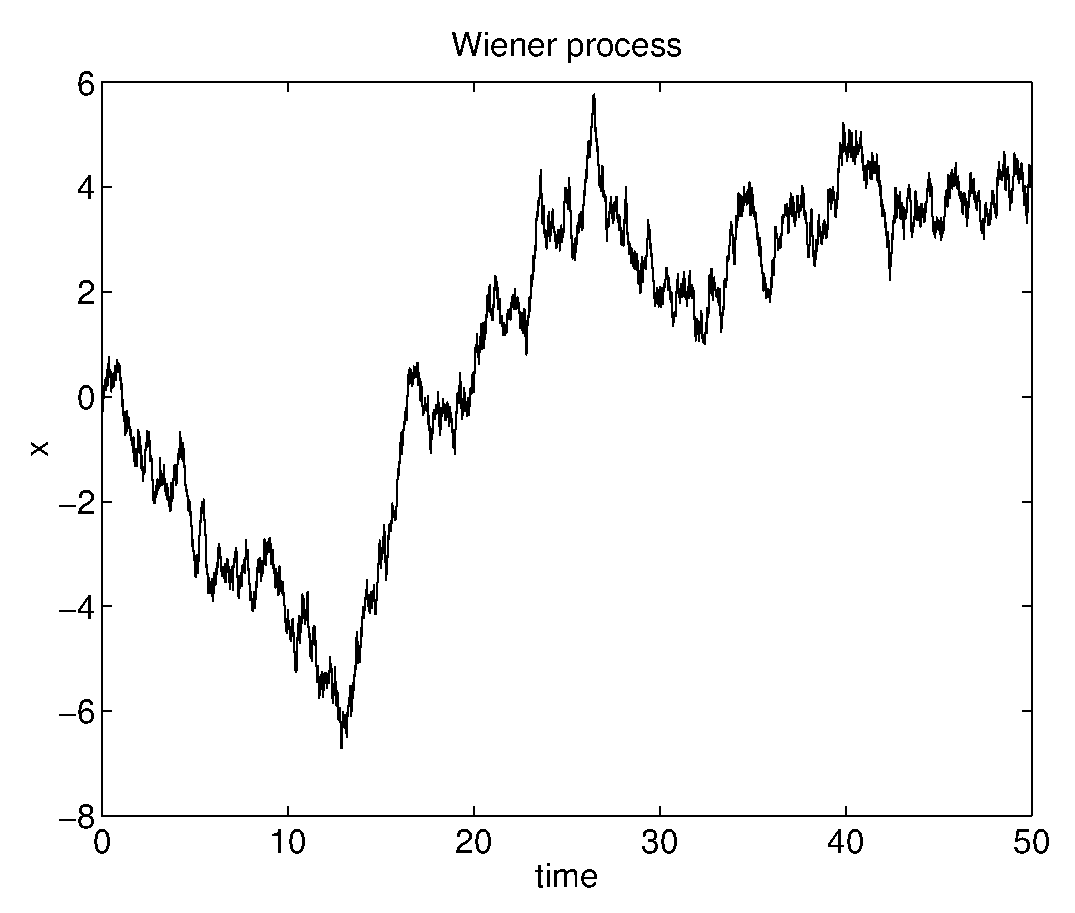
\includegraphics[width=10cm]{./Figures/f_wiener_r1.eps}
\caption{One realization of the Wiener process.
The parameters used in the simulation are \texttt{xstart=0},
\texttt{tend=50}, \texttt{deltat=0.01}, and \texttt{nreal=1}.}
\end{figure}
\begin{figure}
\label{F_WIENER_R2}
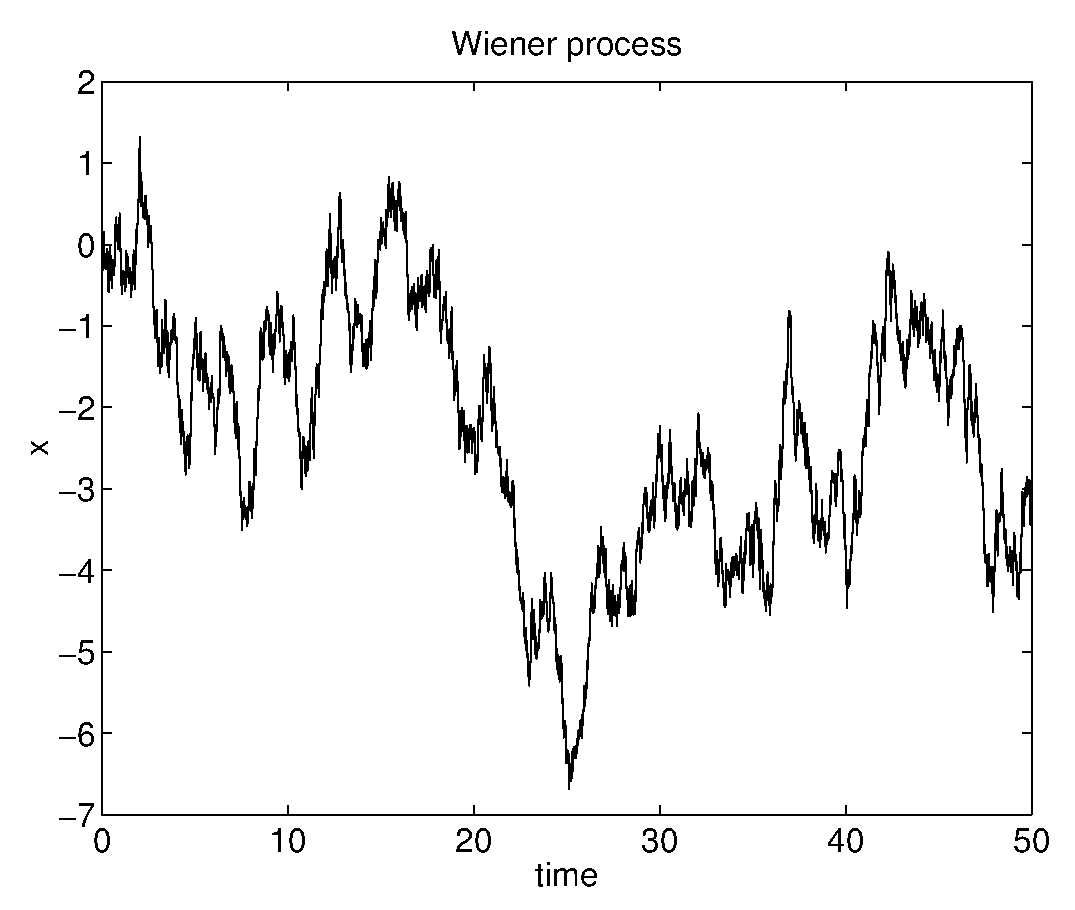
\includegraphics[width=10cm]{./Figures/f_wiener_r2.eps}
\caption{One realization of the Wiener process.
The parameters used in the simulation are \texttt{xstart=0},
\texttt{tend=50}, \texttt{deltat=0.01}, and \texttt{nreal=1}.}
\end{figure}
In Fig. (\ref{F_WIENER}) we show an ensemble average of the
Wiener process over 1000 realizations.
\begin{figure}
\label{F_WIENER}
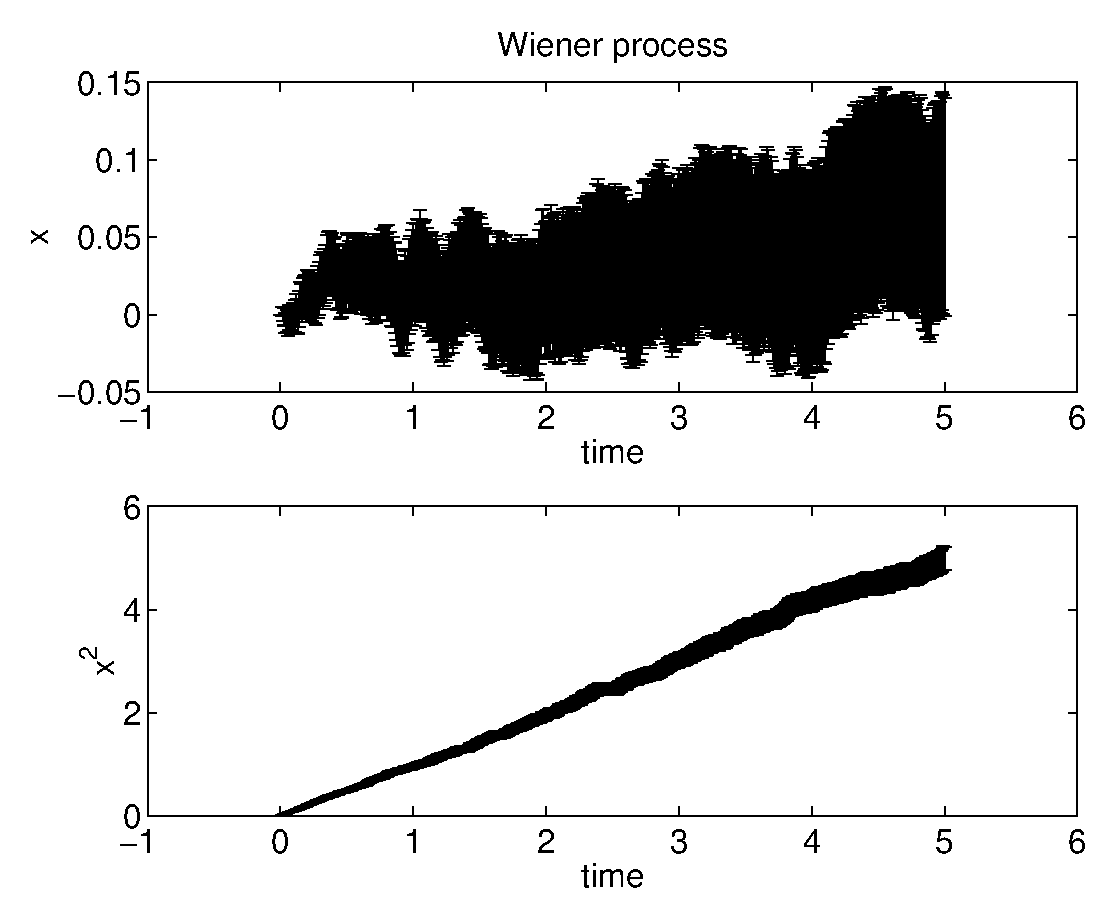
\includegraphics[width=10cm]{./Figures/f_wiener.eps}
\caption{One realization of the Wiener process.
The parameters used in the simulation are \texttt{xstart=0},
\texttt{tend=5}, \texttt{deltat=0.01}, and \texttt{nreal=1000}.}
\end{figure}

\subsection{The Ornstein--Uhlenbeck Process}
Up to now we have considered only Fokker--Planck equations 
without drift. 
As a simple example of a Fokker--Planck equation with an 
additional linear drift we consider
\begin{equation}
\label{ORNSTEIN}
\frac{\partial}{\partial t} T(x,t|x',t') = 
\frac{\partial}{\partial x} [qx T(x,t|x',t')] 
+ \frac{1}{2} D \frac{\partial^2}{\partial x^2} T(x,t|x',t').
\end{equation}
The above Fokker--Planck equation defines the Ornstein--Uhlenbeck
process. 

Again, we can look at the equation of motion for the characteristic
function of the Ornstein--Uhlenbeck process
\begin{equation*}
G(s,t) = \int_{-\infty}^{\infty} dx \exp(isx) T(x,t|x',t').
\end{equation*}
The equation reads
\begin{equation*}
\frac{\partial}{\partial t}G(s,t) = -qs \frac{\partial}{\partial s} 
G(s,t) - \frac{1}{2} Ds^2 G(s,t).
\end{equation*}
The above partial differential equation may be solved by the 
method of characteristics (\cite{gardiner}). Its solution
for $T(x,t_0|x_0,t_0)=\delta(x-x_0)$ requires the
initial condition 
\begin{equation*}
G(s,0) = \exp(ix_0s)
\end{equation*}
and reads
\begin{equation*}
G(s,t) = \exp\left[ -\frac{Ds^2}{4q}[1-\exp(-2q(t-t_0))] + 
 isx'\exp(-q(t-t_0)) 
\right].
\end{equation*}
Hence, the transition probability $T(x,t|x',0)$ is a Gaussian
with mean
\begin{equation}
\label{MEAN_ORNSTEIN}
\langle X(t) \rangle = x_0\exp(-q(t-t_0))
\end{equation}
and variance
\begin{equation}
\label{VAR_ORNSTEIN}
\text{Var} \{ X(t) \} = \frac{D}{2q} [1- \exp(-2q(t-t_0))].
\end{equation}
Since the Ornstein--Uhlenbeck process is a Gaussian process we can write
\begin{equation*}
X(t) = {\bf N}(X_0\exp(-2q(t-t_0)), 
     \frac{D}{2q} (1-\exp(-2q(t-t_0)) ).
\end{equation*}
In contrast to the Wiener process the Ornstein--Uhlenbeck process
has a stationary distribution in the limit $t\longrightarrow \infty$
which is a Gaussian with zero mean and variance $D/2q$.



We now turn to the numerical simulation of realizations of the 
Ornstein--Uhlenbeck process. The problem is to find a way of
determining  from the value of the process $X$ at time $t$
its value at a later time $t+\Delta t$. As for the generation of 
trajectories of the Wiener process it is possible to construct
an update formula for the Ornstein--Uhlenbeck process which is 
exact for any positive value of the time increment $\Delta t$
(\cite{GILLESPIE96}). In order to derive an update formula we
replace in Eqs. (\ref{MEAN_ORNSTEIN}) and (\ref{VAR_ORNSTEIN})
for the mean and variance of the Ornstein--Uhlenbeck process
$t$ by $t+\Delta t$ and $t_0$ by $t$ and accordingly $x_0$ by
$X(t)$. Since we know that the Ornstein--Uhlenbeck process
is Gaussian distributed it is now clear that the update
formula reads
\begin{equation}
X(t+\Delta t) = X(t) \exp(-qt) 
+ \left[ \frac{D}{2q} [1-exp(-2q\Delta t)] \right]^{1/2} \xi,
\end{equation}
where $\xi$ is a Gaussian distributed random number with zero 
mean and unit variance. Since we know how to generate Gaussian 
distributed random numbers the algorithm for the generation of 
realizations of the Ornstein--Uhlenbeck process with diffusion constant
$D$ and inverse relaxation time $q$ reads

(i) Specify the values of $D$, $q$, $x_0$, $\Delta t$.

(ii) Compute the constant coefficients 
\begin{equation*}
\mu \equiv \exp(-q \Delta t)
\end{equation*}
and
\begin{equation*}
\sigma \equiv \left[ \frac{D}{2q} [1-exp(-2q\Delta t)] 
\right]^{1/2}.
\end{equation*}

(iii) Initialize setting $X=x_0$ and $t=0$.

(iv) Replace $t$ by $t+\Delta t$. Terminate the simulation if $t$
exceeed $t_{\text{end}}$.

(v) Generate a Gaussian distributed random number $\xi$ and 
update the process replacing $X$ by $\mu X + \sigma \xi$.

(vi) Goto (iv).

In Fig. (??) we show the flow diagram of the program 
\texttt{ornstein.m} which will be used to generate the 
realizations. The listing of the program can be seen below.

\subsubsection{Listing of the program \texttt{ornstein.m}}
\inputlisting{./Listings/ornstein.m}

One realization of the Ornstein--Uhlenbeck process generated with 
help of the algorithm we have just constructed can be seen in Fig.
(\ref{F_ORNSTEIN_R})

\begin{figure}
\label{F_ORNSTEIN_R}
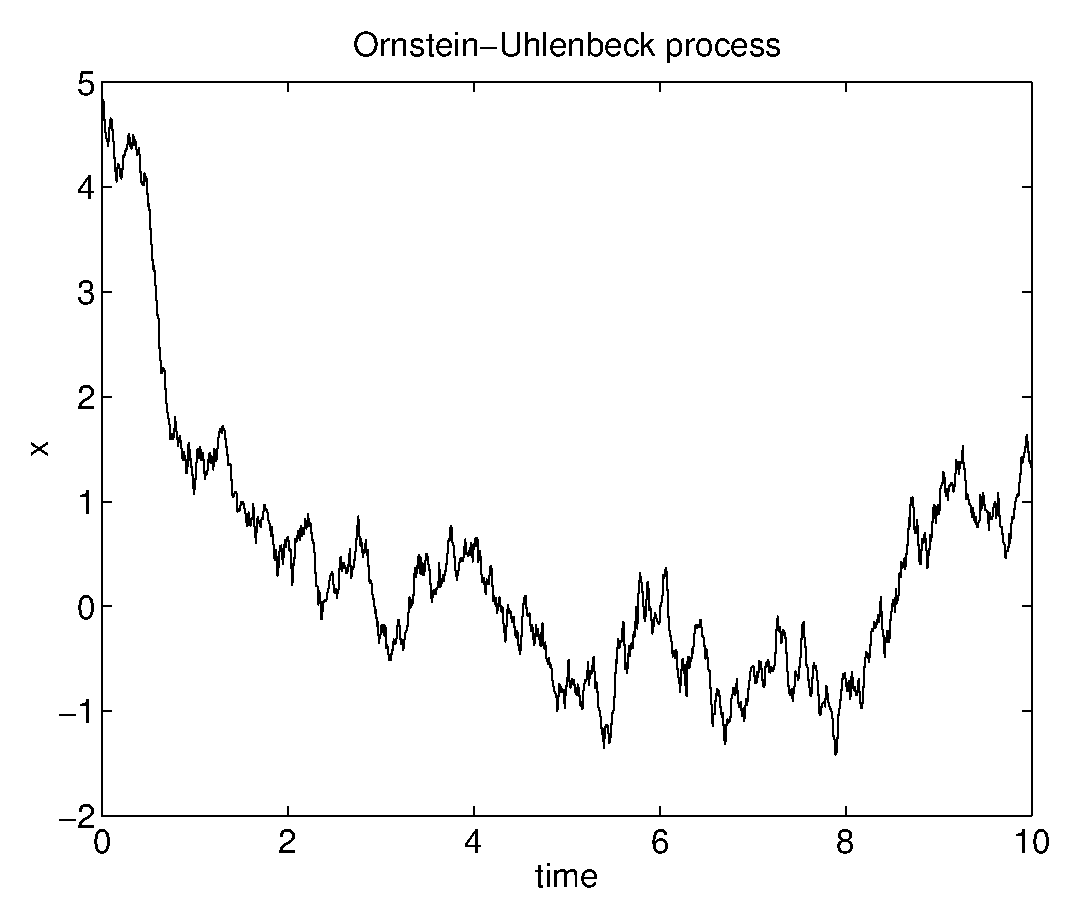
\includegraphics[width=10cm]{./Figures/f_ornstein_r.eps}
\caption{One realization of the Ornstein--Uhlenbeck process. The
 parameters used in the simulation are \texttt{xstart=5},
\texttt{tend=10}, \texttt{deltat=0.01}, \texttt{nreal=1},
\texttt{q=1}, and \texttt{D=1}.}
\end{figure}

The average over 10 realizations of the Ornstein--Uhlenbeck 
process can be seen in Fig. (\ref{F_ORNSTEIN}).
\begin{figure}
\label{F_ORNSTEIN}
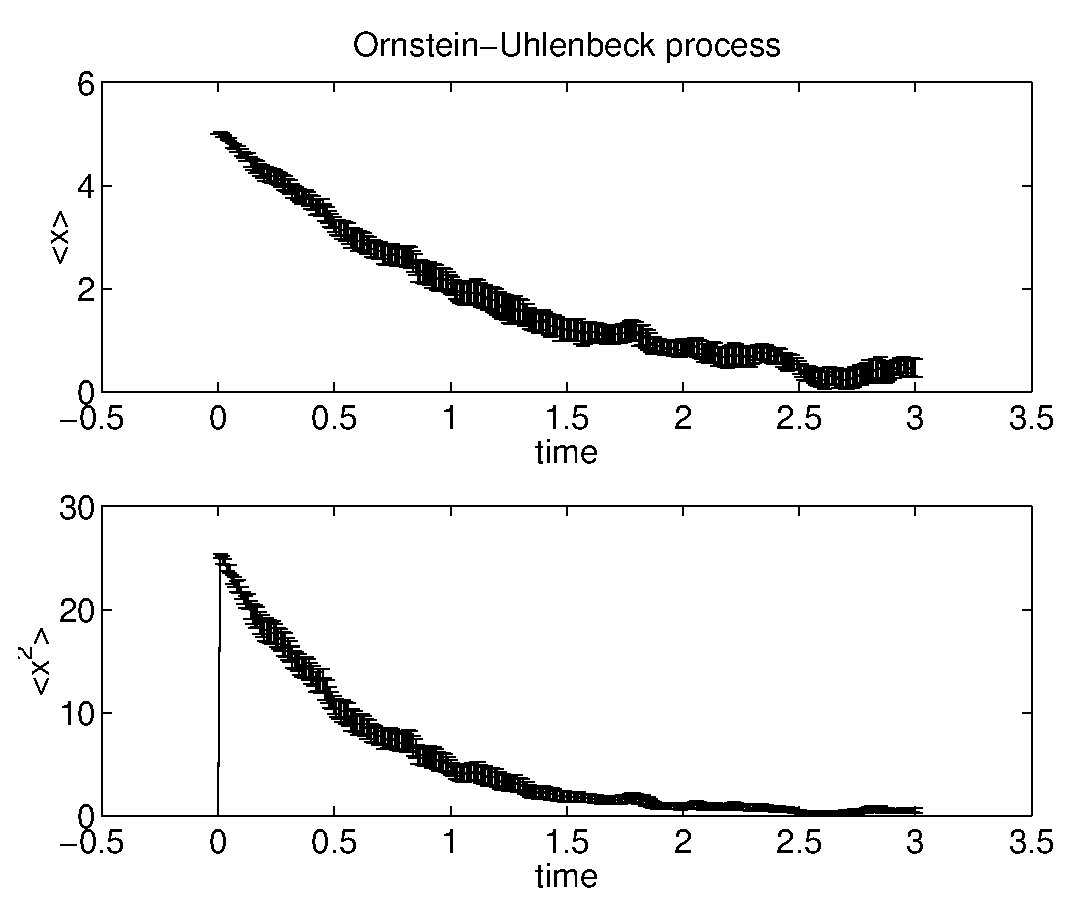
\includegraphics[width=10cm]{./Figures/f_ornstein.eps}
\caption{The average over 10 realizations of the Ornstein--Uhlenbeck 
process. The
 parameters used in the simulation are \texttt{xstart=5},
\texttt{tend=50}, \texttt{deltat=0.01}, \texttt{nreal=10},
\texttt{q=1}, and \texttt{D=1}.}
\end{figure}

%%%%%%%%%%%%%%%%%%%%%%%%%%%%%%%%%%%%%%%%%%%%%%%%%%%%%%%%%%%%%%%%%%%
%%%%%%%%%%%%%%%%%%%%%%%%%%%%%%%%%%%%%%%%%%%%%%%%%%%%%%%%%%%%%%%%%%
\section{Exercises}

\begin{Ex}
\label{Linear_One_Step}
\textbf{Linear one-step process - quantized harmonic oscillator in a %
    radiation field  \cite[page 143]{kampen}} \\
Let $n=0,1,2.\ldots$ numerate the state of a quantized harmonic oscillator 
with energy $h\nu(n+1/2).$ Transitions between the states are induced by the
interaction of the oscillator with the radiation field. The transition 
probability is given by the dipole moments. The only allowed transitions
according to the dipole moments are from $n$ to $n+1$ and from $n$ to $n-1$
(see quantum mechanics lecture).

Therefore the transition rates (probabilities per unit time) are:
\begin{itemize}
\item $g(n-1)=\beta n$ for the transition $(n-1) \rightarrow n$ and
\item $r(n)=\alpha n$ for the transition $n \rightarrow (n-1).$
\end{itemize}
$\alpha$ and $\beta$ are two constants, which depend only on the radiation
density at the frequency $\nu$ and not on $n.$ 

Finally the Master equation for this special one-step process reads
$$ \frac{\partial}{\partial t} P(n,t) = \alpha n P(n+1,t) +\beta(n+1)P(n-1,t)
     -(\alpha n+\beta(n+1))P(n,t).$$

Write a program to simulate the given Master-equation for the one-step
process using the numerical scheme, learned in the lecture.
Choose the parameters $\alpha$ and $\beta$. The result should be a
plot of $P(n,t)$ for different $n$. Plot also $P(n)$ at large $t$, which 
gives the distribution of the
harmonic oscillators with $n$ (and therefore the energy) in the steady state.

The exact stationary solution of the Master-equation
is $P_S(n)= \text{const} \cdot \left(\frac{\beta}{\alpha}\right)^n.$ 
\end{Ex}

\begin{Ex}
\label{Nonlinear_One_Step}
\textbf{Non-linear one-step process - growth of a competitive %
    population \cite[page 163]{kampen} } \\
The number of individuals of some species is called $n.$ The death rate for
this population is $\alpha$ and the birth rate (e.g. by fission)
is $\beta.$ $\alpha$ and $\beta$ are fixed and independent of the
age, otherwise it would not be a Markov process. Both rates are per unit time.

This would be still a linear one-step process. So consider an additional
rate: the competition rate between the individuals of the population.
This rate is an additional death rate and is $\gamma(n-1).$

Therefore the transition rates (probabilities per unit time) are:
\begin{itemize}
\item $g(n)=\beta n$ for the transition $n\rightarrow n+1$
\item $r(n)=\alpha n+\gamma n(n-1)$ for the transition $n \rightarrow n-1.$
\end{itemize}
$\alpha$, $\beta$ and $\gamma$ are constants, which do not depend on $n.$

Finally the Master equation for this one-step process reads
$$ \frac{\partial}{\partial t} P(n,t) = (\alpha n+\gamma n(n-1))P(n+1,t) +
     \beta n P(n-1,t) - (\alpha n+\beta n+\gamma n(n-1))P(n,t).$$

Write again a program to simulate the Master equation and again choose suitable
parameters $\alpha, \beta,\gamma.$ View the time dependence of the population $n$
and try to find out the behaviour of the stationary solutions.

The equation for the first moment (so called macroscopic equation) is called
the {\em Malthus-Verhulst equation} and reads
$$ \dot{<n>} = (\beta-\alpha)<n>-\gamma <n>^2.$$
If you neglect the nonlinear term on the right hand side, 
you get {\em Malthus law}. Then
the solution is just an exponential growth of the population. 

The solutions to the nonlinear equation can be calculated and you get
$$ <n>=\frac{\beta-\alpha}{\gamma} \quad\text{and}\quad <n>\equiv 0 ,$$
where the first one is the stable solution (a so called attractor) 
and the second one is unstable.

{\em example parameters:} $\alpha=0.5, \beta=1, \gamma=0.05 .$
\end{Ex}

\begin{Ex}
\label{Random_Telegraph}
\textbf{The Random Telegraph Process \cite[page 77]{gardiner}} \\
The Random-Telegraph process is the most simple Markov-process possible.
It is a discrete process, which has only two possible states, called
$n=0$ and $n=1$. The master-equation reads
\begin{eqnarray}
 \frac{\partial}{\partial t} P(0,t\mid n'') &= bP(1,t\mid n'')-aP(0,t\mid n'') \\
 \frac{\partial}{\partial t} P(1,t\mid n'') &= aP(0,t\mid n'')-bP(1,t\mid n''). \\
\end{eqnarray}
$a$ and $b$ are the transition rates from state $0\rightarrow 1$
and $1\rightarrow 0$. Examples of this equation are processes, which jump
from one state to the other and back (e.g. spin flipping). 

We can rewrite the two above equations into one equation, resulting in 
the familiar master-equation - DO IT. (you have to ????)
Then write a program to
simulate the master-equation. Use $n=1$ as the initial condition.
For the long time behavior - the stationary solution - the initial
condition is not significant. Try different settings for 
the parameters $a$ and $b$.

Compare the results of the simulation with the exact analytical results.
For $t\to\infty$ the stationary solution for the first moment is:
$$ P(0)=\frac{b}{a+b}, \quad P(1)=\frac{a}{a+b} ,$$  
and
$$ <n> = \sum_{n=0}^1 nP(n)=P(1)=\frac{a}{a+b} .$$
And for the stationary covariance (for the second moment set $t=t'$) 
we get $(t\ge t')$
$$ <n(t)n(t')> = \left(\frac{a}{a+b}\right)^2+\frac{ab}{(a+b)^2}
        e^{-(a+b)(t-t')} .$$

{\em Comment:} This is an example of an ergodic process (a process with
identical ensemble mean and time mean), where you can 
explicitly prove the ergodicity. 
Because if the correlation time is finite, the
system is ergodic. And in this case the correlation time is
$$t_C := \frac{1}{\text{var}(n(0))}\int_0^\infty dt |\text{var}(n(t))| = 
              \frac{1}{(a+b)}$$ 
and therefore finite.
\end{Ex}

\begin{Ex}
\label{Monomolecular_Reaction}
\textbf{Monomolecular Chemical Reaction $A \leftrightarrows X$  %
       \cite[page 183]{schnakenberg} } \\
A further example of a discrete one-step process is a chemical reaction,
where an atom can be either bound to a molecule (call it state X) 
or be by itself (call it state A). We assume that we have an A-reservoir,
so that there are always enough atoms to become absorbed by a molecule. 
The number of molecules (state X) is called $N$, the number of atoms $A.$ 
Another example of
this situation would be an atom in the ground state at a given temperature.
The atom jumps to a higher state and back, depending on the temperature;
assuming low temperatures (A-reservoir).

For chemical reactions the transition rates are given by the rate-constant
$k$, depending on the temperature. The derivation is based on the 
Sto�zahlansatz. So the transition of atoms to molecules is proportional
to the number of atoms in the reservoir $A$ and the transition of molecules
releasing an atom is proportional to the number of molecules $N.$
$$ W_{N+1,N} = A \quad \text{and} \quad W_{N-1,N} = kN .$$

Then the master-equation is
$$ \frac{\partial}{\partial t} P(N,t) = AP(N-1,t)+k(N+1)P(N+1,t)-(A+kN)P(N,t).$$

Again write a program to simulate the master-equation. Use $k=1, A=100$ for
the parameters and $N(0)=A$ as initial value.
Then compare the simulation results with the analytical results:
$$ <N(t)> = A+ (<N(0)>-A)e^{-t} \longrightarrow A \quad\text{for}\quad 
                 t\to\infty,$$
$$ P_{\text{stat}}(N) = \frac{A^N}{N!} e^{-kA} \qquad 
          \text{Poisson-distribution} . $$ 
Also try different parameters and initial conditions.

{\em Comment:} In this example we assumed that there is enough time for the 
reactants to diffuse in the volume. That means the diffusion of atoms and 
molecules is very fast compared to the time a reaction takes place.
If the two time scales are almost the same, we also have to simulate
the diffusion. Such systems are known as reaction-diffusion systems
- we will discuss them later on.
\end{Ex}

\begin{Ex}
\label{Payroll}

\end{Ex}

%%%%%%%%%%%%%%%%%%%%%%%%%%%%%%%%%%%%%%%%%%%%%%%%%%%%%%%%%%%%%%%%%%%%%


\bibliographystyle{peter}
\bibliography{V_98,simulit}

%%%%%%%%%%%%%%%%%%%%%%%%%%%%%%%%%%%%%%%%%%%%%%%%%%%%%%%%%%%%%%%%%%
%%%%%%%% Ende von Kap. 4 %%%%%%%%%%%%%%%%%%%%
%%%%%%%%%%%%%%%%%%%%%%%%%%%%%%%%%%%%%%%%%%%%%%%%%%%%%%%%%%%%%%%%%%%%%


%%% Chapter 5 

\chapter{Stochastic Differential Equations}

In the previous section we have derived an exact simulation algorithm
for the generation of trajectories of the Ornstein--Uhlenbeck process.
The ``exact'' update formula was
\begin{equation*}
X(t+\Delta t) = X(t) \exp(-q \Delta t) +
  \left[ \frac{D}{2q}(1-\exp(-2q\Delta t)) \right]^{1/2} \xi(t),
\end{equation*}
where we have now written $\xi(t)$ to stress the fact that at each
time step $t$ we have to draw another Gaussian distributed random 
number. The update formula is exact in the sense that it holds for
arbitrary values of $\Delta t$.

However, it will turn out to be convenient to have an update formula
which works for small values of $\Delta t$. To this end we expand the
exact update formula to first order in $\Delta t$ and obtain
\begin{eqnarray}
X(t+\Delta t)& =& X(t) (1- q \Delta t) + 
   \left[ \frac{D}{2q} (2q \Delta t) \right]^{1/2} \xi(t) \nonumber
   \\
\label{SDE_APPROX} 
  & = & X(t) - qX(t) \Delta t + \sqrt{D} \sqrt{\Delta t} \xi(t).
\end{eqnarray}
In the limit $\Delta t \rightarrow 0$ this approximate update formula
turns exact.  We recognize immediately that the stochastic increment in
this discretized version of the Ornstein--Uhlenbeck process scales
with the square root of the time increment $\Delta t$.

Note that in deriving the above discretized update formula we have 
intentionally omitted the terms linear in $\Delta t$ stemming from 
the expansion of the factor in front of the stochastic term. In 
doing so we have achieved that the update formula has an important
property. Namely, it is selfconsistent in the following sense
(\cite{GILLESPIE}). Let us apply the above formula twice, starting from,
\begin{equation*}
X(t+2\Delta t) = X(t+\Delta t) 
 - qX(t+ \Delta t) \Delta t + \sqrt{D} \sqrt{\Delta t} \xi(t+\Delta t).
\end{equation*}
Inserting (\ref{SDE_APPROX}) we immediately obtain keeping 
terms up to first order in $\Delta t$
\begin{equation*}
X(t+2 \Delta t) = X(t) - q X(t) 2 \Delta t +
   \sqrt{D} \sqrt{\Delta t} [\xi(t) + \xi(t+\Delta t)].
\end{equation*}
Since $\xi(t)$ and $\xi(t+\Delta)$ are statistically independent
Gaussian stochastic processes we have
\begin{equation*}
\xi(t) + \xi(t+\Delta t) = {\bf N}(0,1) + {\bf N}(0,1) =
  {\bf N}(0,2) = \sqrt{2} {\bf N}(0,1),
\end{equation*}
so that we finally have
\begin{equation*}
X(t+2 \Delta t) = X(t) - q X(t) 2 \Delta t +
   \sqrt{D} \sqrt{2 \Delta t} \xi(t).
\end{equation*}
This selfconsistency of the discretized stochastic differential 
equation expresses essentially the fundamental properties
of the propagator of a Markov process as they are defined in
the Chapman--Kolmogorov equation.


Due to the presence of a stochastic term, the Gaussain stochastic
process $\xi(t)$, the above equation is a discretized version of a 
so--called {\em stochastic differential equation} (SDE). It is the aim
of this section to introduce into some  peculiarities of stochastic
differential equations. In particular we will also show the
equivalence of stochastic processes defined in terms of stochastic differential
equations and in terms of Fokker--Planck equations.

The above expression is a special case of the  {\em standard form} of
a stochastic differential equation (some times stochastic
differential equations are also called {\em Langevin} equations):
\begin{equation}
\label{SDE_LANGEVIN_DISCR}
X(t+dt) = X(t) + A(X(t),t)dt + \sqrt{D(X(t),t)} \xi(t) dt^{1/2},
\end{equation}
where we have replaced $\Delta t$  by $dt$ to stress the infinitesimal
character of the above equation. The term proportional to $dt$ is
called the {\em drift term}, whereas the term proportional to
$\sqrt{dt}$ is called the diffusion term. 

The above definition of the stochastic process $X(t)$
in terms of a stochastic differential equation  cleary shows that
the stochastic process $X(t)$ is continuous, but, in general, not 
differentiable. This can be seen by writing
Eq. (\ref{SDE_LANGEVIN_DISCR}) as
\begin{equation*}
\label{eq:XiinSDE}
\frac{X(t+dt) - X(t)}{dt} = A(X(t),t) + \frac{\sqrt{D(X(t),t)} \xi(t)}
                                              {\sqrt{dt}}.
\end{equation*}
Obviously, the limit $dt \rightarrow 0$ of the above equation does not
exist, unless $D\equiv 0$. Thus, a purely stochastic Markov process
is everywhere continuous but nowhere differentiable. Nevertheless it is
customary in the physical literature to ``pretend'' (\cite{GILLESPIE})
that $dx/dt$ exists even for
non vanishing $D$. In fact we know that we can write (see section
\ref{sec:WienerProcess})
\begin{equation*}
\frac{\xi(t)}{\sqrt{dt}} = \frac{1}{\sqrt{dt}} {\bf N}(0,1) =
{\bf N}(0,1/dt).
\end{equation*}
So, we may define a Gaussian {\em white noise process} as
\begin{equation*}
\eta(t) \equiv \lim_{dt \rightarrow 0}  {\bf N}(0,1/dt).
\end{equation*}
With the help of the above definition, we can now formally write
(compare with \ref{eq:XiinSDE})
\begin{equation*}
\frac{d}{dt} X(t) = A(X(t),t) + \sqrt{D(X(t),t)} \eta(t).
\end{equation*}
This equation is called the white noise form of the Langevin equation.
The white noise process introduced above does have the following
averaged properties:
\begin{eqnarray*}
\langle \eta(t) \rangle &=& 0 \\
\langle \eta(t) \eta(t') \rangle &=& \delta(t-t'),
\end{eqnarray*}
which satisfy the requirement of no correlation at different
times. Note, that the white noise process  $\eta$ has
infinite variance. Accordingly, the spectral density, i.e.,
the Fourier transform of the correlation function of $\eta$ is 
constant. This is the reason for calling $\eta$ a white noise
process.

It is important to establish precisely the relationship
between the white noise process and the Wiener process
(\cite{GILLESPIE}).
We know already that the special Wiener process $dW(dt)$
is a normal random variable with mean zero and variance $dt$
\begin{equation*}
dW(dt) = {\bf N}(0,dt).
\end{equation*}
It follows from the theorems of Gaussian probability densities
that
\begin{equation*}
{\bf N}(0,dt) =  dt {\bf N}(0,1/dt).
\end{equation*}
Because of the definition of the Gaussian white noise process we 
can conclude that
\begin{equation*}
dt \eta(t) = dW(dt)
\end{equation*}
and hence we have formally in the limit $dt \rightarrow 0$
\begin{equation*}
\frac{dW}{dt} = \eta(t).
\end{equation*}
This equation asserts that the derivative of the Wiener process is 
the white noise process. However, we know already that the Wiener
process is not differentiable so that the white noise process must 
be ill--defined. We will see shortly how these formal difficulties 
may easily be circumvented in the proper definition
of stochastic differential equations. Before doing so we will 
consider for a 
moment the most classical Langevin equation of statistical 
physics, namely the one describing Brownian motion.

\section{The Langevin Equation and Brownian Motion}
In 1908 Langevin considered the problem of the dynamical 
description of Brownian motion (\cite{VAN_KAMPEN}). 
He suggested that the equation of 
motion of a Brownian particle with mass $m=1$ be described by the
following differential equation for the velocity $V$
\begin{equation}
\label{LANGEVIN}
\frac{d}{dt} V = -\gamma V + L(t),
\end{equation}
where the terms on the right hand--side of the above equation 
model the forces which the surrounding molecules excerpt on the 
Brownian particle. Since these forces are unknown in detail the 
following assumptions were postulated. The Brownian particle 
moving in the fluid of surrounding particles feels
a dissipative drag force which is proportional to its velocity, $\gamma$  being 
the friction coefficient. Furthermore, the Brownian particle hits
the surrounding particles. These collisions cause irregular 
changes in the velocity of the Brownian particle. Thus, the external force
$L(t)$ is modeled as a zero mean, temporally uncorrelated
randomly fluctuating force. The first two moments of the
stochastic process $L(t)$ are assumed to 
have the following properties
\begin{eqnarray*}
\langle L(t) \rangle &=& 0 \\
\langle L(t) L(t') \rangle &=& \Gamma \delta(t-t').
\end{eqnarray*}

The Langevin equation is the prototype of a stochastic 
differential equation, i.e. of a differential equation whose
coefficients are random functions of the time with some given
statistical properties. 
It is clear that choosing $L(t)=\sqrt{\Gamma} \eta(t)$,
where $\eta(t)$ is a Gaussian white noise process, the Langevin 
equation of Brownian motion describes an Ornstein--Uhlenbeck
process.
The stochastic process $V(t)$ is 
completely defined once an initial condition $V(0)=V_0$ is specified.
Its formal solution reads
\begin{equation*}
V(t) = V_0 \exp(-\gamma t) + \exp(-\gamma t) 
    \int_0^t dt' \exp(\gamma t') L(t').
\end{equation*}
Taking the average over an ensemble of Brownian particles all
having the same initial condition we find for the mean value of 
the velocity
\begin{equation*}
\langle V(t) \rangle = V_0 \exp(-\gamma t),
\end{equation*}
where we made use of the statistical properties of the Langevin 
force $L(t)$. Accordingly, the second moment of the velocity field
is found to be
\begin{eqnarray*}
\langle V^2(t) \rangle &=& V_0^2 \exp(-2\gamma t)
          + \exp(-2 \gamma t) \int_0^t dt'' \int_0^t dt'
             \exp(\gamma (t' + t'')) \langle L(t') L(t'') \rangle 
             \\
          &=& V_0^2 \exp(-2\gamma t) + \frac{\Gamma}{2 \gamma}
             [1-\exp(-2 \gamma t)].
\end{eqnarray*}
Up to now the constant $\Gamma$ was left unspecified. From 
equilibrium statistical physics (theorem of equipartition of energy) 
we  expect that for long times 
\begin{equation*}
\langle V^2(t\rightarrow \infty) \rangle = kT.
\end{equation*}
Hence we have
\begin{equation}
\label{FDT1}
\Gamma = 2 \gamma kT
\end{equation}
and we have established a relation between the attrition 
coefficient $\gamma$ and the random fluctuations.
Eq. (\ref{FDT1}) is a simple version of the so--called
fluctuation--dissipation theorem.


\section{Stochastic Integration}
It is the aim of this section to show how the formal problems
arising in the formulation of Langevin equations can be avoided.
Let us begin by formulating the Langevin equation in a discrete 
way,
\begin{equation*}
dX(t) = a(X(t),t) dt + b(X(t),t) \eta(t) dt,
\end{equation*}
where $a(X(t),t)$ is a deterministic drift and $b(X(t),t)$ is the 
diffusion term, $\eta(t)$ being a Gaussian white noise process.
We proceed by integrating the above equation from $t_0$ to $t$
and obtain for each sample path
\begin{equation*}
X(t) = X(t_0) + \int_{t_0}^t ds a(X(s),s) 
+ \int_{t_0}^t b(x(s),s) \eta(s) ds.
\end{equation*}
Since the Wiener process $W(t)$ can be represented as the integral
over a white noise process, i.e.,
\begin{equation}
W(t) = \int_{t_0}^t ds \eta(s)
\end{equation}
the integral form of the Langevin equation can be written as
\begin{equation}
\label{SDE_INTEGRAL}
X(t) = X(t_0) + \int_{t_0}^t ds a(X(s),s) 
+ \int_{t_0}^t b(x(s),s) dW(s).
\end{equation}
The above expression is 
expected to make sense because the Wiener process is continuous. 
We will see shortly that the above 
equation does have a precise meaning. In fact
from here on a solution of a stochastic differential equation will be 
interpreted as a solution 
of the corresponding integral equation, which will be written
in the short--hand notation
\begin{equation*}
dX(t) =   a(X(t),t) dt + b(x(t),t) dW(t).
\end{equation*}

Of course, the second integral in Eq. (\ref{SDE_INTEGRAL}) is not 
an ordinary integral.  It is an integral with respect to the 
Wiener process $W(t)$. Such integrals are called {\em stochastic 
integrals} and we will define and discuss them now. For a precise
mathematical definition of stochastic integrals see \cite{GARD, 
POTTER,KLOEDEN_AN,OETTINGER}. We will follow here the more
{\em physical} line of reasoning of \cite{gardiner}.

\subsection{Definition of the Stochastic Ito Integral}
The starting point for the definition of the Ito integral is the
following reasoning. For $b(X(t),t)=b=\text{const}$, the stochastic 
integral
\begin{equation*}
I = \int_{t_0}^t bdW(s)
\end{equation*}
is expected to be defined and to be equal to
\begin{equation*}
I = b \{ W(t) - W(t_0) \}.
\end{equation*}
In general it seems to be safe to treat the stochastic 
integral 
\begin{equation*}
I(f) = \int_{t_0}^t f(X(s),s) dW(s)
\end{equation*}
as a kind of Riemann--Stieltjes integral, i.e., as a limit of 
partial sums. To do so we divide the interval $[t_0,t]$ into $n$
subintervals
\begin{equation*}
t_0 \le t_1 \le t_2 \le \cdots \le t_{n-1} \le t_n \equiv t
\end{equation*}
and define intermediate points $\tau_i$
\begin{equation*}
t_{i-1} \le \tau_i \le t_i.
\end{equation*}
The stochastic integral $I(f)$ is then defined as the limit
of the partial sums
\begin{equation*}
S_n = \sum_{i=1}^n f(\tau_i) \left[  W(t_i) - W(t_{i-1}) \right].
\end{equation*}
In general it turns out that the definition of the stochastic 
integral depends on the particular choice of the intermediate 
point $\tau_i$. In the definition of the Ito stochastic integral
the intermediate points are chosen to be at the beginning of
the corresponding time interval, i.e.,
\begin{equation*}
\tau_i = t_{i-1}.
\end{equation*}
Accordingly the Ito stochastic integral is defined as the limit of 
the partial sums
\begin{equation*}
S_n = \sum_{i=1}^n f(t_{i-1}) [  W(t_i) - W(t_{i-1}) ].
\end{equation*}
The limit of the sequence of partial sums is to be understood in the
following sense. The random variable $S_n$ is said to converge to $S$
 in the mean square limit if
\begin{equation*}
\lim_{n \rightarrow \infty}
 <(S_n -S)^2> =0.
\end{equation*}
The above limit is usually written as
\begin{equation*}
\text{ms-} \lim_{n \rightarrow \infty} S_n = S.
\end{equation*}
In this sense the Ito stochastic integral of the function $f(t)$ is
defined as
\begin{equation*}
\int_{t_0}^t f(x(t'),t') dW(t') = \text{ms-}\lim_{n \rightarrow \infty}
   \left\{ \sum_{i=1}^{n} f(t_{i-1}) [W(t_i) - W(t_{i-1})] 
   \right\}.
\end{equation*}

\subsection{The Stratonovich Stochastic Integral}
\label{STRATONOVICHSUB}
An alternative definition of a stochastic  integral has been given by
Stratonovich. He suggested the following definition
\begin{equation}
\label{STRATONOVICHDEFI}
S\int_{t_0}^t f(x(t'),t') dW(t') = \text{ms-}\lim_{n \rightarrow \infty}
   \left\{ \sum_{i=1}^{n} f( \frac{x(t_{i})+ x(t_{i-1})}{2}, t_{i-1}) 
[W(t_i) - W(t_{i-1})]   \right\}.
\end{equation}
The $S$ in front of the integral denotes a Stratonovich integral
in contrast to the Ito integral.
Note, that in this definition the integrand is evaluated in an
averaged way.

\subsection{Ito Calculus}
We now want to derive some very useful formulas. In order to do so 
we have to introduce a special class of functions. A function $g(t)$
is called a {\em nonanticipating function} of $t$ if for all
$s$ and $t$ such that $t<s$, $g(t)$ is statistically independent 
of $W(s)-W(t)$. In other words $g(t)$ is independent of the 
behaviour of the Wiener process in the future of $t$. Within the 
context of the stochastic differential equations such functions 
are quite reasonable since they express the fact that the future 
does not affect the present. This guarantees, evidently, 
causality.

We are now in the position to give the proof of the fundamental 
equation of Ito calculus, namely, that
\begin{equation*}
dW(t)^2 = dt 
\end{equation*}
and that
\begin{equation*}
dW(t)^{2+N} =0 
\end{equation*}
for $N \ge 1$. These formulas will allow for a comfortable 
handling of stochastic differentials.

We begin by proofing that
\begin{equation}
\label{PROOFDW2DT}
\int_{t_0}^t \left[ dW(t') \right]^2 g(t') = \int_{t_0}^t dt' 
g(t')
\end{equation}
for a nonanticipating function $g(t)$. By definition of the 
stochastic Ito integral we have
\begin{eqnarray*}
\int_{t_0}^t \left[ dW(t') \right]^2 g(t') & = & 
\text{ms-}\lim_{n \rightarrow \infty} \sum_i g_{i-1} \Delta W_i^2 \\
   & = & \lim_{n \rightarrow \infty} 
    < \left[ \sum_i g_{i-1} \Delta W_i^2 \right]^2>.
\end{eqnarray*}
Eq. (\ref{PROOFDW2DT}) is of course to be understood in the mean
square sense, so we consider the following expression
\begin{eqnarray*}
I & = & \lim_{n \rightarrow \infty} 
< \left[ \sum_i g_{i-1} (\Delta W_i^2  -\Delta t_i)\right]^2   > 
\\
& = & \lim_{n \rightarrow \infty} 
<  \sum_i (g_{i-1})^2 (\Delta W_i^2  -\Delta t_i^2)
+\sum_{i>j} 2 g_{i-1}g_{j-1} (\Delta W_j^2  -\Delta t_j)
 (\Delta W_i^2  -\Delta t_i) >.
\end{eqnarray*}
We can now exploit the fact that in the first sum in the above expression
the $(g_{i-1})^2$ and $(\Delta W_i^2  -\Delta t_i^2)$ and accordingly in the 
second sum $g_{i-1}g_{j-1} (\Delta W_j^2  -\Delta t_j)$ and 
$(\Delta W_i^2  -\Delta t_i)$ are statistically independent from 
each other because the function $g$ is nonanticipating and because 
of the properties of the Wiener process. This statistical 
independence permits to factorize the mean value. So we find
\begin{equation*}
I = 2 \lim_{n \rightarrow \infty} 
\left[ \sum_i \Delta t_i <(g_{i-1})^2> \right],
\end{equation*}
where we have used the following properties of the Wiener process
\begin{equation*}
<\Delta W_i^2> = \Delta t_i
\end{equation*}
and
\begin{equation*}
<(\Delta W_i^2 - \Delta t_i)^2> = 2 \Delta t_i^2.
\end{equation*}
Hence we can conclude that
\begin{equation*}
\text{ms-}\lim_{n \rightarrow} 
\left( \sum_i g_{i-1} \Delta W_i^2 - \sum_i g_{i-1} \Delta t_i \right)
=0.
\end{equation*}
Since 
\begin{equation*}
\text{ms-}\lim_{n\rightarrow \infty} \sum_i g_{i-1} \Delta t_i =
\int_{t_0}^t dt' g(t')
\end{equation*}
we have completed the proof of Eq. (\ref{PROOFDW2DT}).
The importance of Eq. (\ref{PROOFDW2DT}) is the following one. Because
of the definition of stochastic differential equations $dW(t)$
occurs only in integrals, so that we can explicitly write
\begin{equation*}
dW(t)^2 \equiv dt.
\end{equation*}
Accordingly, it is straightforward to show that in the same sense
\begin{equation*}
dW(t)^{2+N} \equiv 0, \;\;\; \text{for} \;\;\; N>0.
\end{equation*}
In the following it will be of some importance to have 
multiplication rules for stochastic differentials. The following
multipication table sums up the rules for products of stochastic 
differntials.
\begin{table}
\caption{Multiplication table for products of stochastic differentials.}
\begin{center}
\begin{tabular}{|c||c|c|c|}\hline 
$\times$ & $dW$ & $dW^2$ & $dt$ \\ \hline \hline
$dW$     & $dt$ & $0$    & $0$   \\ \hline
$dW^2$   &  $0$ & $0$    &  $0$  \\ \hline
$dt$     &  $0$ & $0$    & $0$  \\ \hline
\end{tabular}
\end{center}
\end{table}
As an example of the application of the above formulas we consider the
integration of a polynomial. Let us look at
\begin{eqnarray*}
d[W(t)]^n & = & [W(t) + dW(t)]^n - W(t)^n \\
          & = & \sum_{r=1}^n \binom{n}{r} W(t)^{n-r} dW(t)^r .
\end{eqnarray*}
Using the fact that $dW(t)^r = 0$ for $r>2$ we conclude that
\begin{equation*}
d[W(t)]^n = n W(t)^{n-1}dW(t) +
\frac{n(n-1)}{2} W(t)^{n-2} dt
\end{equation*}
so that
\begin{equation*}
\int_{t_0}^t W(t')^n dW(t') = \frac{1}{n+1}  [W(t)^{n+1} - W(t_0)^{n+1}]
   -\frac{n}{2} \int_{t_0}^t W(t')^{n-1} dt.
\end{equation*}



\section{Ito Stochastic Differential Equations}
Having defined stochastic integrals the proper definition of a
stochastic differential equation can be given (Again we follow 
\cite{gardiner}. The mathematically interested reader should
consult \cite{GARD,KLOEDEN_AN,POTTER}). The stochastic variable
$X(t)$ obeys the Ito stochastic differential equation
\begin{equation}
\label{ITOSDE}
dX(t) = a(X(t),t) dt + b(X(t),t) dW(t)
\end{equation}
if for all $t$ and $t_0$ the following integral equation holds
\begin{equation}
X(t) = X(t_0) + \int_{t_0}^t ds a(X(s),s) 
     + \int_{t_0}^t dW(s) b(X(s),s).
\end{equation}

\subsection{Ito's Formula}
In this subsection we want to consider a function
$f$ of the stochastic variable $X(t)$ and derive an Ito stochastic
differential equation for $f$. We begin by expanding the differential 
$df(x(t))$ to second order in $dW(t)$
\begin{eqnarray*}
df(X(t)) & = & f(X(t)+dX(t)) - f(X(t)) \\
         & = & f'(X(t)) dX(t) + \frac{1}{2} f''(X(t)) dX(t)^2 + \ldots.
\end{eqnarray*}
Inserting the Ito stochastic differential equation (\ref{ITOSDE})
for $dX(t)$ we get
\begin{eqnarray*}
df(X(t)) &=&  f'(X(t)) \{a(X(t),t)dt + b(X(t),t) dW(t) \} \\
      & & + \frac{1}{2} f''(X(t)) b(X(t),t)^2 [dW(t)]^2 + \ldots ,
\end{eqnarray*}
where we have discarded all other terms of higher order. Using
finally $[dW(t)]^2 =dt$ we get
\begin{eqnarray}
\label{ITOFORMULA}
df(X(t)) &=& \{a(X(t),t) f'(X(t)) +  \frac{1}{2} f''(X(t)) b(X(t),t)^2
\} dt  \nonumber \\
    & & + b(X(t),t)f'(X(t)) dW(t).
\end{eqnarray}
The above equation is Ito's formula and expresses the fact that 
in general for stochastic differential equations
the change of variables is not given by the rules of 
ordinary calculus.


\subsection{The Equivalence of Stochastic Differential Equations 
  and of the Fokker--Planck Equation}
Let us now look at the time development of the expectation value 
of an arbitrary function
$f(X(t))$.
Using Ito's formula we immediately have
\begin{eqnarray*}
\frac{<df(X(t))>}{dt} & = & \left< \frac{df(X(t))}{dt} \right> = 
               \frac{d}{dt} <f(X(t)) > \\
       & = & < a(X(t),t) f'(X(t)) +   \frac{1}{2} f''(X(t)) b(X(t),t)^2   >.
\end{eqnarray*} 
Since, $X(t)$ is a Markov process it does have a conditional
probability density $T(x,t|x_0,t_0)$ and accordingly we can write
\begin{eqnarray*}
\frac{d}{dt} <f(X(t)) > &=& \int dx f(x) \frac{\partial}{\partial t} 
         T(x,t|x_0,t_0) \\
          & = & \int dx 
       [a(X(t),t) f'(X(t)) +   \frac{1}{2} f''(X(t)) b(X(t),t)^2] T(x,t|x_0,t_0).
\end{eqnarray*}
The above equation can now be integrated by parts. Disregarding
surface terms we obtain
\begin{equation*}
\int dx f(x) \frac{\partial}{\partial t} T = \int dx f(x)
   \{ - \frac{\partial}{\partial x}[a(x,t)T] + \frac{1}{2} 
        \frac{\partial^2}{\partial x^2}[b(x,t)^2 T] \}.
\end{equation*}
Since, by construction $f$ is an arbitrary function of $x$ we can
conclude that
\begin{equation*}
 \frac{\partial}{\partial t} T(x,t|x_0,t_0) =
    - \frac{\partial}{\partial x}[a(x,t)T(x,t|x_0,t_0)] + \frac{1}{2} 
        \frac{\partial^2}{\partial x^2}[b(x,t)^2 T(x,t|x_0,t_0)].
\end{equation*}
We immediately recognize that the above equation is a Fokker--Planck
equation. Hence we have shown the equivalence of a diffusion
process defined in terms of a stochastic differential equation with
drift coefficient $a(x(t),t)$ and a diffusion coefficient
$b(X(t),t)^2$ and the above Fokker--Planck equation.

\section{The Stratonovich Stochastic Differential Equation}
In subsection \ref{STRATONOVICHSUB} we have seen that it is 
possible to give other definitions of the stochastic integral.
One such definition is the Stratonovich stochastic integral defined 
in Eq. (\ref{STRATONOVICHDEFI}). It is clear that it is then possible 
to define stochastic differential equations using the 
Stratonovich integral, i.e.,
\begin{equation}
\label{STRATOSDE}
X(t) = X(t_0) + \int_{t_0}^t ds \alpha(x(s),s) +
      S \int_{t_0}^t dW(s) \beta(x(s),s).
\end{equation}
In the mathematical literature it is customary to write
the Stratonovich integral in the form
\begin{equation*}
\int_{t_0}^t  \beta(x(s),s) \circ dW(s) 
\equiv S\int_{t_0}^t  \beta(x(s),s) dW(s) ,
\end{equation*}
where the notation $\circ$ is called the {\em Ito circle}. From
here on we will also stick to this notation.
It is the aim of this subsection to show that stochastic 
differential equations defined in terms of the Stratonovich 
integral are equivalent to some appropriate Ito stochastic 
differential equations.

To this end we assume that the above $x(t)$ is also a solution of the Ito 
stochastic differential equation
\begin{equation}
\label{ITOSDEINS}
dx(t) = a(x(t),t) dt + b(x(t),t) dW(t)
\end{equation}
and try to derive expressions for the corresponding $\alpha$ and $\beta$
in Eq. (\ref{STRATOSDE}).

We begin by establishing the relation between the Ito and the 
Stratonovich integral. By definition of the Stratonovich integral 
we have
\begin{equation}
\label{STRATOIAPP}
\int_{t_0}^t  \beta(x(s),s) \circ dW(s) \approx
 \sum_i \beta \left( \frac{x(t_i) + x(t_{i-1})}{2},t_{i-1} \right)
  [W(t_i) -W(t_{i-1})].
\end{equation}
Using
\begin{equation*}
x(t_i) = x(t_{i-1}) + dx(t_{i-1})
\end{equation*}
the argument of the $\beta$ function can be written as
\begin{equation*}
\beta \left( \frac{x(t_i) + x(t_{i-1})}{2},t_{i-1} \right) =
 \beta \left( x(t_{i-1}) + \frac{1}{2} dx(t_{i-1}) ,t_{i-1}\right).
\end{equation*}
Then, with the help of the Ito stochastic differential equation 
(\ref{ITOSDEINS}) in the form
\begin{equation*}
dx(t_i) = a(x(t_{i-1}),t_{i-1}) (t_i -t_{i-1}) + 
   b(x(t_{i-1}),t_{i-1}) (W(t_i) -W(t_{i-1}))
\end{equation*}
and of Ito's formula we get
\begin{eqnarray*}
\beta \left( \frac{x(t_i) + x(t_{i-1})}{2},t_{i-1} \right) & = &
 \beta(t_{i-1}) + \left[ a(t_{i-1}) \frac{\partial}{\partial x} 
 \beta(t_{i-1}) + \frac{1}{4} b^2(t_{i-1})
                  \right] \frac{1}{2}(t_{i} - t_{i-1}) \\
 &  + & \frac{1}{2} b(t_{i-1}) \frac{\partial}{\partial x} 
 \beta(t_{i-1}) [W(t_i) - W(t_{i-1})].
\end{eqnarray*}
The above expression can now be inserted back into the Eq. 
(\ref{STRATOIAPP}). Exploiting the fact that Ito calculus allows us to set 
$dW^2=dt$ and to drop the terms $dt^2$ and $dtdW$ we find
\begin{eqnarray*}
\int_{t_0}^t  \beta(x(s),s) \circ dW(s) & \approx &
\sum_i \beta(x(t_{i-1}),t_{i-1}) [W(t_i) - W(t_{i-1})] \\
 &  + & \frac{1}{2} \sum_i b(x(t_{i-1}),t_{i-1}) 
 \frac{\partial}{\partial x} \beta(x(t_{i-1}),t_{i-1}) (t_i - 
 t_{i-1}).
\end{eqnarray*}
Since the first term on the right side of the above equation is a
partial sum of an Ito integral we conclude from the above discrete
formula that
\begin{equation}
\int_{t_0}^t  \beta(x(s),s) \circ dW(s) = 
\int  \beta(x(t'),t') dW(t') 
 + \frac{1}{2} \int b(x(t'),t') 
 \frac{\partial}{\partial x} \beta(x(t'),t') dt'.
\end{equation}
The above formula gives us the relation between the Ito and the 
Stratonovich integral of a function $\beta(x(t),t)$ in which $x(t)$
is the solution of the Ito stochastic differential equation
(\ref{ITOSDEINS}). The relation between the Ito and the 
Stratonovich form of stochastic differential equations can be seen 
by setting
\begin{eqnarray*}
\alpha(x(t),t) & = & a(x(t),t) - \frac{1}{2} b(x(t),t) 
\frac{\partial}{\partial x} b(x(t),t), \\
\beta(x(t),t) & = & b(x(t),t).
\end{eqnarray*}
We then get the following important equivalence.

The Ito stochastic differential equation
\begin{equation}
dx = a dt + b dW(t)
\end{equation}
is equivalent to the Stratonovich stochastic differential equation
\begin{equation}
dx = [a- \frac{1}{2} b \frac{\partial}{\partial x}b] dt + b \circ 
dW(t).
\end{equation}
Conversely, the Stratonovich stochastic differential equation
\begin{equation*}
dx = \alpha dt + \beta \circ dW(t)
\end{equation*}
is equivalent to the Ito stochastic differential equation
\begin{equation*}
dx = [\alpha + \frac{1}{2} \beta \frac{\partial}{\partial x} 
\beta]dt + \beta dW(t).
\end{equation*}

\subsection{Ito or Stratonovich?}
We have just seen that a given stochastic differential 
equation can be interpreted in two ways: in the sense of Ito and 
in the sense of Stratonovich. Each of the two interpretations can be converted
equivalently in the other version of the stochastic differential 
equation. Thus, the question arises: When modeling a physical 
system which interpretation should we use? 

At the basis of the problem is the fact that 
in the {\em more physical} Langevin equations we are confronted
with a $\delta$ correlated white noise process.
Hence, the proper 
mathematical analysis of stochastic differential equations was based 
on the {\em mathematically safe} Wiener process and we were led
automatically to the ambiguities of defining Riemann sums for 
stochastic integrals.

All these difficulties can be circumvented by the following 
reasoning. Real processes in nature do have finite correlation 
times. Their spectrum might be flat, but not up to infinite 
frequencies. Such a noise term is called colored  noise and could 
have zero mean and the following correlation function
\begin{equation*}
< \eta(t) \eta(t+\tau) > = \frac{\sigma^2}{2m} \exp(- m |\tau|).
\end{equation*}
The corresponding colored noise Langevin equation would read
\begin{equation}
\dot{X}(t) = a(X(t),t) + b(X(t),t) \eta(t).
\end{equation}
For such a colored noise process the Riemann sums do converge and 
no ambiguity exists in choosing an interpretation.

In other words the ambiguities vanish by performing first the 
integration of the above colored noise Langevin equation and then 
perform the white noise limit $\sigma \rightarrow \sigma m$ and 
$m \rightarrow \infty$. Proceeding in this way we automatically 
get the Stratonovich interpretation of the stochastic differential 
equation. This is the content of the Wong-Zakai theorem 
(\cite{HORSTHEMKE}). A good discussion of the Ito--Stratonovich
dilemma can be found in \cite{VAN_KAMPEN}.



\section[The Euler--Maruyama Method]%
{The numerical integration of stochastic differential 
equations: The Euler--Maruyama method}
Let us begin this section by review some basic facts of numerical 
methods for the simulation of {\em deterministic} ordinary 
differential equations (\cite{GARCIA,PRESS}). 
To this end we consider the initial value 
problem
\begin{eqnarray*}
\frac{dx}{dt} &=& a(t,x), \\
   x(t_0) & = & x_0.
\end{eqnarray*}
The most widely used numerical algorithms for the solution of the 
above problem are \index{finite differences} techniques. The simplest such 
method is the \index{Euler method}. The basic idea of the Euler 
method is to approximate the derivative on the right hand of the 
differential equation by the first order approximation
\begin{equation*}
\frac{dx}{dt} = \frac{x(t+\Delta t) - x(t)}{\Delta t} + O(\Delta 
t).
\end{equation*}
An approximate solution of the initial value problem can then be 
constructed by iterating the following recursion relation
\begin{equation*}
x(t+\Delta t) = x(t) + a(t,x)\Delta t.
\end{equation*}
Alternatively, introducing the time discretization
$t_0 < t_1 < \ldots t_n$ with equal increments $\Delta t$
the Euler algorithm can be formulated as
\begin{equation}
\label{EULERODE}
x_{n+1} = x_{n} + a(t_n,x_n) \Delta t,
\end{equation}
where it is intended that $x_n = x(t_n)$. Once, the initial value 
$x_0$ has been specified the approximation $x_1, x_2, \ldots, x_n$ 
can be determined by applying Eq. (\ref{EULERODE}) recursively.


Let us now turn our attention to the easiest finite difference 
method for the integration of stochastic differential equations
\cite{HONERKAMP,KLOEDEN_NUM,OETTINGER}.
Essentially, we have already met the easiest method for the 
numerical integration of stochastic differential equation while 
motivating them at the beginning of this chapter.
Assume that we are interested in the solution of the following
initial value problem for an Ito stochastic differential equation
\begin{eqnarray*}
dX(t) &=& a(X(t),t) dt + b(X(t),t) dW(t), \\
X(t_0) &=& X_0,
\end{eqnarray*}
where $X_0$ is the initial condition at time $t_0$. The simplest 
discretization scheme for the above differential equation
is the Euler scheme, which in the context of stochastic 
differential equations is sometimes called the Euler--Maruyama
method. For a given partition 
$t_0 < t_1 < \cdots < t_{n-1} < t_n=t_{end}$ 
the Euler scheme is given by
\begin{eqnarray*}
\tilde{X}_n &=& \tilde{X}_{n-1} +a (\tilde{X}_{n-1},t_{n-1}) \Delta 
t_n + b(\tilde{X}_{n-1},t_{n-1}) \Delta W_n, \\
\tilde{X_0} &=& X_0,
\end{eqnarray*}
where $\Delta t_n = t_n - t_{n-1}$ and $\Delta W_n$
is the Wiener increment
\begin{equation*}
\Delta W_n = W(t_n) - W(t_{n-1}).
\end{equation*}
Usually, we have $\Delta t_n = \Delta t = \text{const}$, so that
we can generate the Wiener increment with the help of the formula
\begin{equation*}
\Delta W_n = \xi \sqrt{\Delta t},
\end{equation*}
where $\xi$ is a gaussian distributed random variable with mean 
zero and unit variance. The random variable $\tilde{X}_n$ 
generated by this iterative scheme is expected to approximate the 
stochastic process $X(t)$. Sometimes the above scheme is also 
termed the stochastic difference equation associated with the 
corresponding stochastic differential equation.

In order to characterize the quality of the approximation schemes 
for stochastic differential equations we have to introduce the 
concept of strong convergence. We say that a discrete 
approximation $\tilde{X}$ with maximum time step $\Delta t$
converges strongly to $X$ at time $t_{end}$ if
\begin{equation*}
\lim_{\Delta t \rightarrow 0} <|X(t_{end}) - \tilde{X}(t_{end})|> 
=0.
\end{equation*}
The order of convergence $\nu$ determines the numerical efficiency
of a given numerical approximation scheme. If there exists a 
positive constant $c$, which is independent of $\Delta t$ such 
that for sufficiently small $\delta t$ we have
\begin{equation*}
<|X(t_{end}) - \tilde{X}(t_{end})|^2>^{1/2} \le c (\Delta t)^{\nu},
\end{equation*}
then we say that the approximation scheme converges strongly with
order $\nu$. 
The above criterion is simply the generalization of the usual 
deterministic convergence criterion and reduces to it when the 
diffusion coefficient vanishes and the initial condition is
deterministic (\cite{KLOEDEN_AN}). 
The concept of a strongly  convergent scheme is relevant for the
following reason: A strongly convergent scheme gives 
approximations to the individual trajectories of the 
stochastic process. This is very important when the simulation is 
expected to resolve characteristic features of the trajectories of 
a stochastic process.

It can be shown that the Euler scheme  has strong 
order of convergence $\nu = 0.5$. Thus the oder of strong 
convergence of the stochastic Euler scheme is quite poor.

Fortunately, quite often one is not interested in constructing the 
individual realizations of the stochastic process but only in some 
averaged quantities, e.g., in some moments of the stochastic 
process. This is always the case, if the stochastic differential 
equation is regarded as an efficient numerical tool for the
solution of a given Fokker--Planck equation. Namely, the latter 
contains only information about the moments of the stochastic 
process and not about the trajectories themselves. In these cases
one is interested in the {\em weak} solutions of stochastic 
differential equations. An approximation scheme is said to 
converge weakly with order $\nu$ at time $t_{end}$ if for 
sufficiently smooth functions $g$ there exists a positive constant 
$c$, which does not depend on $\Delta t$ such that for 
sufficiently small $\Delta t$ we have
\begin{equation*}
|<g(X(t_{end})> - <g(\tilde{X}(t_{end}))>| \le c (\Delta t)^{\nu}.
\end{equation*}
Under suitable smoothness conditions for the functions $g$ the 
Euler scheme can be shown to have order of weak convergence 
$\nu=1$.

\subsection{The Ornstein-Uhlenbeck Process}
As a first example of the application of the Euler algorithm
we consider again the Ornstein--Uhlenbeck process.
The implementation of the stochastic Euler algorithm has been 
realized in the program \texttt{sdeornstein}.

\subsubsection{Listing of the program \texttt{sdeornstein.m}}
\inputlisting{./Listings/sdeornstein.m}

The algorithm is very similar to the algorithm for the generation 
of exact trajectories of the Ornstein--Uhlenbeck process. 
Instead of looking at the realizations we estimate the expectation
value for $<X^2>$ at the fixed final time \texttt{tend=4} 
(\texttt{tstart=0}). Choosing $q=1$ and $D=1$ the exact value of
$<X^2(t=4)>$ is expected to be
\begin{equation*}
<X^2(t=4)> = \frac{1}{2}(1-\exp(-8)) = 0.4998.
\end{equation*}
Since we know from the general discussion of the Euler algorithm
that the expectation values converge to the exact result linearly 
with the time step we have included in the program a \texttt{for}
loop over \texttt{istep} time steps \texttt{deltat} to see explicitly this
dependence. At the end of the simulation we perform a linear fit
of the results with the help of the function \texttt{polyfit} in 
order to be able to extrapolate the results to $\Delta t =0$.

The results of the simulation for 50.000 realizations 
and \texttt{deltat=0.2, 0.1, 0.05, 0.025} are summarized in the following 
table 
\begin{table}
\caption{Results of the simulation of the Ornstein--Uhlenbeck 
process with the stochastic Euler method for different values of 
the time step. The parameters of the Ornstein-Uhlenbeck process
are \texttt{q=1}, \texttt{D=1}. The simulation was run from
\texttt{tstart=0} to \texttt{tend=4} for 50000 realizations.
The timesteps used are \texttt{deltat=0.2, 0.1, 0.05, 0.025}.}
\begin{center}
\begin{tabular}{|c|c|c|} \hline \hline
$\Delta t$ & $<X^2>$ & $\sigma$ \\ \hline \hline
0.2      & 0.557979 & 0.00354552 \\ \hline
0.1      & 0.523506 & 0.00331771  \\ \hline
0.05     & 0.511591 & 0.00322181  \\ \hline
0.025    & 0.506859 & 0.00320129  \\ \hline \hline
\end{tabular}
\end{center}
\end{table}
The same data have been plotted in Fig. (\ref{F_SDEORN_50}).
\begin{figure}
\label{F_SDEORN_50}
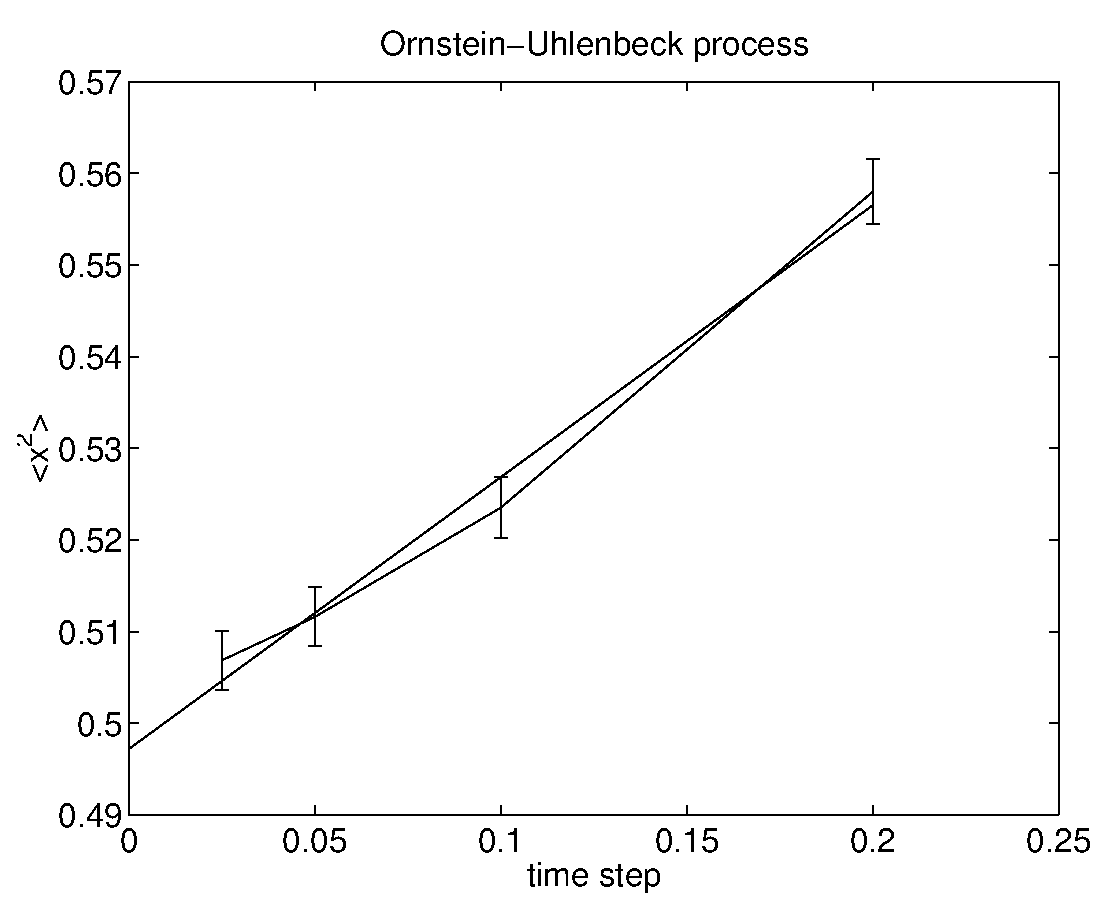
\includegraphics[width=10cm]{./Figures/f_sdeorn_50.eps}
\caption{Results of the simulation of the Ornstein--Uhlenbeck 
process with the stochastic Euler method for different values of 
the time step. The parameters of the Ornstein-Uhlenbeck process
are \texttt{q=1}, \texttt{D=1}. The simulation was run from
\texttt{tstart=0} to \texttt{tend=4} for 50000 realizations.
The timesteps used are \texttt{deltat=0.2, 0.1, 0.05, 0.025}.} 
\end{figure}
The figure clearly shows the expected linear convergence of the 
estimate to the expected exact result. The linear extrapolation 
leads to the estimate $<X^2>|_{t=4}=0.497182$, which is in very 
good agreement with the expected exact result. The simulation took
1729 sec on the laptop.

\subsection{Noise Induced Transitions}
In this second example of the application of the stochastic Euler 
method we want to simulate a stochastic differential equation with
multiplicative noise and consider noise induced transitions.

Let us begin by looking at the following deterministic dynamical 
system
\begin{equation*}
\frac{d}{dt} x(t) = \frac{1}{2} - x(t),
\end{equation*}
for $x \in [0,1]$. Obviously, this dynamical system has one 
fix point at $x_0=1/2$. This fix point can be shown to be 
asymptotically stable. 

We now want to perturb this system by adding a multiplicative 
noise term on the right hand of the above equation of motion.
To be precise we want to replace the deterministic equation of 
motion by the Ito stochastic differential equation
\begin{equation}
\label{SDENOISEIN}
dX(t) = (\frac{1}{2} - X(t))X(t)dt + \epsilon X(t) (1-X(t)) dW(t),
\end{equation}
where $\epsilon <0$

In order to understand the results of the simulation  we want to 
look at the stationary solution of the corresponding 
Fokker--Planck equation. The latter reads
\begin{equation*}
\frac{\partial}{\partial t} = - \frac{\partial}{\partial x} [a(X(t)) P(X,t) ]
      + \frac{1}{2} \frac{\partial^2}{\partial 
      x^2}[b(X(t))P(X,t)],
\end{equation*}
where we have used
\begin{equation*}
a(X(t)) = \left(\frac{1}{2} - X(t)\right) X(t)
\end{equation*}
and
\begin{equation*}
b(X(t)) = [\epsilon X(t) (1-X(t))]^2.
\end{equation*}
Of course, the stationary solution has to satisfy
\begin{equation*}
\lim_{t \rightarrow \infty} \frac{\partial}{\partial t} P(X,t) =0
\end{equation*}
and hence
\begin{equation*}
\frac{d}{dx} [a(X(t)) P(X,t) ] - \frac{1}{2} \frac{\partial^2}{\partial 
      x^2}[b(X(t))P(X,t)] =0.
\end{equation*}
The above equation can be written as
\begin{equation}
\label{DDXJ}
\frac{d}{dx} J(x) =0,
\end{equation}
with 
\begin{equation*}
J(x) = a(X(t)) P(X,t)  - \frac{1}{2} \frac{\partial}{\partial 
      x}[b(X(t))P(X,t)].
\end{equation*}
In order to satisfy Eq. (\ref{DDXJ}) $J$ must be constant. If we 
assume that the stationary density $P_S(x) \longrightarrow 0$ for 
$|x| \longrightarrow \infty$ then the constant in question must be 
zero and we can conclude that
\begin{equation*}
\frac{d}{dx} [b(x) P_S(x)] = 2 a(X)P_S(x).
\end{equation*}
Dividing both sides by $b(x)P_S(x)$ we get
\begin{equation*}
\frac{d [b(x) P_S(x)]}{b(x) P_S(x)} = \frac{2a(x)}{b(x)}.
\end{equation*}
Integrating the above expression gives
\begin{equation*}
\ln [b(x) P_S(x)] = \int_c^x dx' \frac{2a(x')}{b(x')}
\end{equation*}
or
\begin{equation*}
P_S(x) = \frac{N}{b(x)} \exp\{-\phi (x)\},
\end{equation*}
where
\begin{equation*}
\phi(x) = - \int_c^x dx' \frac{2a(x')}{b(x')}.
\end{equation*}
The factor $N$ is a normalization constant to be chosen such that
\begin{equation*}
\int_a^b P_S(x) dx =1.
\end{equation*}

Transposing the above sketched general theory to the stochastic 
differential equation of interest  we get the stationary density,
which is sometimes also called the invariant density,
\begin{equation*}
P_S(x) = \frac{N}{x(1-x)} \exp\left( - \frac{1}
           {\epsilon^2 x(1-x)}\right)
\end{equation*}

Now we are in the position to simulate the stochastic differential
equation (\ref{SDENOISEIN}). This will be done with the help of 
the program \texttt{sdenoisein.m}.

\subsubsection{Listing of the program \texttt{sdenoisein.m}}
\inputlisting{./Listings/sdenoisein.m}
The program generates trajectories of the stochastic process with 
the help of the Euler algorithm. At the end of the simulation we evaluate 
numerically the stationary distribution with the help
of the MATLAB plotting function \texttt{hist}.

In a first run we perform a simulation of 5000 trajectories for 
the following parameters \texttt{xstart=0.5}, \texttt{epsilon=1},
\texttt{tend=4}, and \texttt{deltat=0.01}. The initial condition
was always chosen to be \texttt{xstart=0.5}. The resulting histogram
of the invariant density can be seen in Fig. 
(\ref{F_SDENOISEIN_1}).

\begin{figure}
\label{F_SDENOISEIN_1}
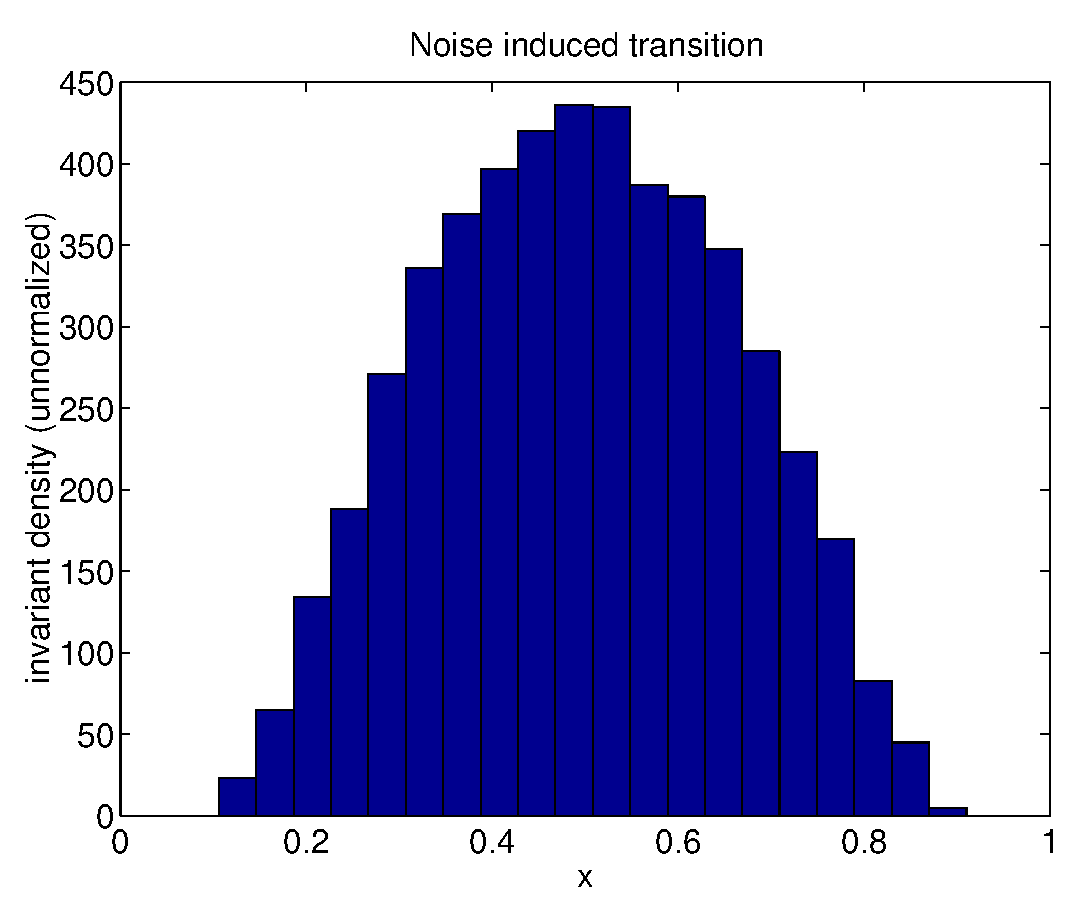
\includegraphics[width=10cm]{./Figures/f_sdenoisein_1.eps}
\caption{Histogram of the invariant density of the stochastic differential 
equation with multiolicative noise. The simulation was run from
\texttt{tstart=0} to \texttt{tend=4} for 5000 realizations.
The initial condition was chosen to be \texttt{xstart=0.5}.
The timestep used was \texttt{deltat=0.01} and the multiplicative noise 
constant was \texttt{epsilon=1}.} 
\end{figure}

It is clear from the histogram that the most probable value of $X$ 
lies around 0.5 and is therefore identical with the fixed point of 
the corresponding deterministic process.

Now we run the program with the same parameters as above but 
choose the multiplicative noise constant to be \texttt{epsilon=3}.
The result of this second simulation can be seen in Fig. 
(\ref{F_SDENOISEIN_2}).
\begin{figure}
\label{F_SDENOISEIN_2}
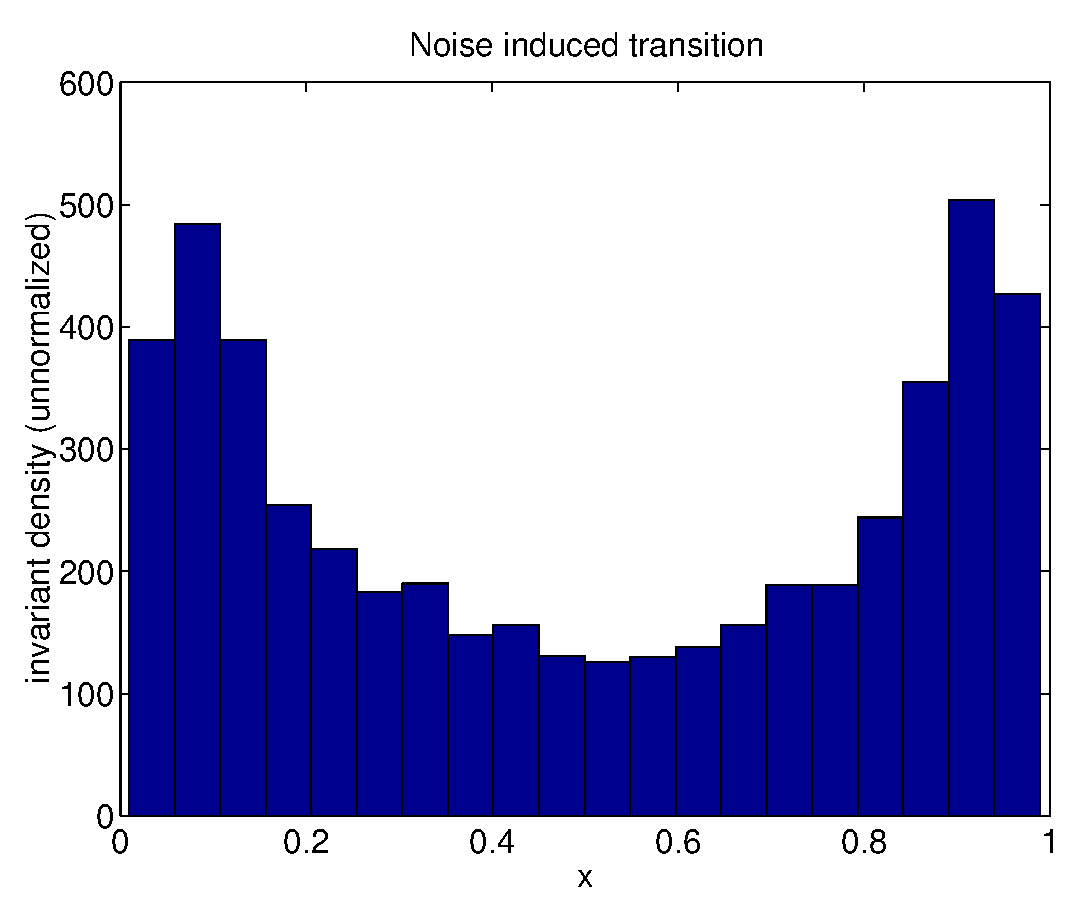
\includegraphics[width=10cm]{./Figures/f_sdenoisein_2.eps}
\caption{Histogram of the invariant density of the stochastic differential 
equation with multiolicative noise. The simulation was run from
\texttt{tstart=0} to \texttt{tend=4} for 5000 realizations.
The initial condition was chosen to be \texttt{xstart=0.5}.
The timestep used was \texttt{deltat=0.01} and the multiplicative noise 
constant was \texttt{epsilon=3}.} 
\end{figure}
It is evident from this figure that the invariant density changes 
its character. Now there is no longer one value of $X$ which is 
more probable. The histogram shows a minimum for $X=0.5$ and two 
equally high maxima at around 0.1 and 0.9. As a consequence of 
the larger noise the system undergoes a "stochastic bifurcation" 
which changes the number of the maxima of the invariant density. 
Such a phenomenon is called a {\em noise induced transition}.

Let us now try to see whether this observation is in agreement 
with the stationary density we have derived at the beginning of 
this subsection. The maxima of the stationary distribution are 
easily evaluated from the equation
\begin{equation*}
0 = \frac{d}{dx}P_S(x_m)
\end{equation*}
which explicitly reads
\begin{equation*}
0= (1-2x_m) [1- \epsilon^2 x_m (1-x_m) ].
\end{equation*}
For $0 < \epsilon <2$ the invariant density has an extremum, 
namley a maximum at $x_m =x_0= 1/2$, which is the fixed point of the 
deterministic equation of motion. For $\epsilon > 2$ the invariant
density posses a minimum at $x_0 =1/2$ and two maxima of equal 
height at $x_{m1,m2}$
\begin{equation*}
x_{m1,m2} = \frac{1}{2} \left(1 \pm  \sqrt{1 - (4/\epsilon^2)} 
\right).
\end{equation*}
Thus for the value of \texttt{epsilon=3} chosen in the second 
simulation the maxima are expected  to be at 0.8727 and 0.1273 
respectively. The histogram reproduced in Fig. (\ref{F_SDENOISEIN_2})
is in agreement with this theoretical prediction.


\section{Stochastic Resonance}
In order to get aquainted with 
the numerical integration of stochastic differential equations we discuss a
phenomenon which occurs as
the response of a nonlinear system in the presence of noise: stochastic 
resonance. For a comprehensive introduction see \cite{Lanzara,Bulsara}. 
We already know that the effect of noise on the time evolution of 
deteministic linear system is rather trivial. If the statistical properties of
the input noise are known it is straightforward to compute the statistical
properties of the output signal. For nonlinear systems the situation changes
dramatically. The presence of the noise influences the evolution of the
system often in a counterintuitive way. The numerical integration of the
corresponding stochastic differential equations allows us to look at the
realizations of the process and to gain insight in these interesting
phenomena. 

The phenomenon of stochastic resonance was proposed by Benzi \textit{et al.}
\cite{Benzi1,Benzi2} in a series of papers in which they address the problem
of the periodic switching of the Earth's climate between periods of relative
warmth and ice ages. It is known from the statistical analysis of continental
ice volume over the last million years that this switching is random and that 
it occurs with an approximate period of 100000 years. It is as well known that
the eccentricity of the Earth orbit varies with roughly the same period. 
However,
the associated variations of the solar energy influx on the earth surface are
so small, that climatologists doubt that  such a small external periodic force
effect might induce such climatic changes. In their seminal papers Benzi
\textit{et al.} represent the global climate with the help of a bistable
``climatic potential''. One minimum of the potential represents a small
temperture typical of an ice age, the other one a more  warm climate.
These authors then show that the weak periodic variation of the eccentricity
together with other random perturbations modelled as additive noise (e.g.
short--term climate fluctuations) might explain the periodicity observed for
the transition between one and the other of the two stable climate 
states. They name this
phenomenon stochastic resonance for the following reason: the
signal--to--noise ratio, i.e. the response of the system, is maximized when a
parameter of the stochastic force is tuned to an optimal value.

It is the aim of this section to introduce the basic principles of stochastic
resonance \cite{McNamara,Gammaitoni} and to simulate a simple model 
showing this phenomenon.
It is clear from the example discussed above that the basic mechanism  of 
stochastic resonance relies upon three essential ingredients:
a bistable system, a periodic driving signal, and a noise signal.

The simplest version of a one--dimensional nonlinear dynamical system 
is the damped anharmonic oscillator with the following equation of motion
\begin{equation}
m \frac{d^2x}{dt^2} + \gamma \frac{dx}{dt} = - \frac{dU(x)}{dx} 
 + \sqrt{D} \chi(t).
\end{equation}
The above Langevin equation describes the motion of a classical particle of
mass $m$ in a potential $U(x)$ and with an additive stochastic force
$\chi(t)$,
where $\chi(t)$
is a Gaussian white noise characterized by
\begin{equation}
\langle \chi(t) \rangle =0; \;\;\; \langle \chi(t) \chi(t')\rangle =
\delta(t - t').
\end{equation}
The potential $U$ is bistable and we assume that it has the simple form
(see figure \ref{fig:BistablePotential})
\begin{equation}
U(x) = -a \frac{x^2}{2} + b \frac{x^4}{4}.
\end{equation}
\begin{figure}[htbp]
  \begin{center}
    \includegraphics[width=\textwidth]{Figures/BistablePotential.eps}
    \caption{The potential $U(x)=-a \frac{x^2}{2} + b \frac{x^4}{4}$ 
      for $a=1$ and $b=1$.}
    \label{fig:BistablePotential}
  \end{center}
\end{figure}
For $a> 0$ the potential $U$ is bistable with an unstable state at $x=0$
and two stable states at $x_s = \pm \sqrt{a/b}$. The stable states are
separated by a barrier of height $\Delta U = a^2/4b$. The system remains
dynamically stable for $b>0$, and becomes monostable for $a \le 0$.
Furthermore we assume that the system is overdamped by neglecting the inertial
term $m d^2x/dt^2$. 
Rescaling the resulting Langevin equation with the damping constant
$\gamma$  we finally obtain the so--called stochastic Ginzburg--Landau
equation
\begin{equation}
\label{Stoch_Ginzburg_Landau}
\frac{dx(t)}{dt} = ax - bx^3 + \sqrt{D} \chi(t),
\end{equation}
an equation which is often encountered in the theory of nonequilibrium
critical phenomena. 

\subsection{Reaction Rate Theory}
Let us now investigate some fundamental properties of the above dynamical
system. We begin by considering the case $D=0$ (no fluctuations). If the 
system is initially in a stable state it remains there for ever. 
The typical local
time scale is the relaxation time $\tau_r$ inside the wells. This time scale 
can be determined by considering small variations around the 
minimum of the well.
To do so we linearize Eq. (\ref{Stoch_Ginzburg_Landau}) 
around the stable state $x_s = \sqrt{a/b}$ with the help of
\begin{equation}
x(t) = x_s + \delta x(t)
\end{equation}
and obtain
\begin{equation}
\frac{d(\delta x)}{dt} = -2a \delta x.
\end{equation}
Thus, the  time scale $\tau_r$ of the relaxation inside the wells is
\begin{equation}
  \tau_r = \frac{1}{2a} = \frac{1}{U''(x_s)}.
\end{equation}

The situation changes in the presence of noise. The fluctuating forces allow
the system to jump between the two stable states. If the noise strength $D$ 
is small compared to the barrier height, these jumps are rare events. 
It is a well--know result of Kramers reaction--rate theory (see e.g.
\cite{Haenggi:Kramers}) that the mean escape time $T_e(x)$ out of one basin of
attraction can be written for sufficiently low noise ($\Delta U/D \gg 1$)in 
the form of the Arrhenius law
\begin{equation}
  \label{eq:Arrhenius}
  T_e(x) = A \exp(\Delta U(x)/D),
\end{equation}
where $A$ is a prefactor which depends on the form of the potential. For the
special potential we consider here, performing a Gaussian approximation of the
potentail around the minimum and the maximum and using the condition
$\Delta U/ D >> 1$ one gets the so--called Kramers
formula (or Arrhenius formula) for the escape time of a bistable system
\begin{equation}
\label{eq:Kramers}
  \tau_k = \frac{2\pi}{\sqrt{|U''(0)|U''(x_s)}} \exp [ 2 \Delta U / D ].
\end{equation}
The escape time $\tau_k$ is the global time scale of the bistable system.
The physical content of the assumptions we stated above is the following
one: The Kramers time $\tau_k$ is derived under the assumption that the
probability density within a well is roughly in equilibrium when the escape
takes place. Thus, the condition $\Delta U/D \gg 1$ guarantees that the two
time scales, the relaxation time and the Kramers time are different. The
system relaxes quickly (on a short time scale) to a local equilibrium at the
stable states and approaches global equilibrium (transitions over the barrier)
on a slow time scale. It follows from Eq. (\ref{eq:Kramers}) that
\begin{equation}
  \frac{\tau_k}{\tau_r} = 2 \sqrt{2} \pi \exp(2 \Delta U /D) \gg 1.
\end{equation}
The rate to jump over the barrier $W_k$ is obviously the inverse escape time
\begin{equation}
  w_k = \tau_k^{-1} = \frac{a}{\sqrt{2} \pi} \exp(-2 \Delta U/D).
\end{equation}

\subsection{The Stochastic Resonance}
Having reviewed some basic results of the theory of nonlinear stochastic
systems we are now ready to look at the phenomenon of stochastic resonance.
In the preceeding subsections we made use only of two of the basic ingredients
of the recipe for stochastic resonance. The phenomenon only occurs in the
presence of a periodic driving signal. If we add such a signal to the bistable
system just considered its dynamics will be governed by the following Langevin
equation
\begin{equation}
  \frac{dx}{dt} = - \frac{\partial U(x,t)}{\partial x} + \sqrt{D} \chi(t), 
\end{equation}
where the bistable potential takes now the form
\begin{equation}
\label{eq:bistablepotential}
  U(x,t) = -a \frac{x^2}{2} +b \frac{x^4}{4} - Ax \cos(\omega_s t),
\end{equation}
where $A$ and $\omega_s= 2 \pi/T_s$ are the amplitude 
and the frequency of the periodic
signal. As a consequence of the periodic forcing term the potential tilts
periodically between up  and down. When the periodic force is at its
maximum (or minimum)  the difference between the escape rates from the two
states is maximum. The periodic forcing is assumed to be so
weak that it can not let the particle roll periodically from one potential
well into the other one. Nevertheless, the noise--induced hopping beween the
two wells  may become synchronized with the weak periodic forcing. This is 
signature of stochastic resonance. Stochastic resonance manifests itself by a
synchronization of activated hopping between the potential minima with the
weak periodic forcing. 

The manifestation of the phenomenon may be visualized with the help of the
output signal. It is clear that in the absence of the periodic driving
the escape process is induced by the fluctuating force and is random. Thus, in
this case the output signal $x(t)$ looks like dichotomous noise. The
probability density of residence times between two jumps is exponential
\begin{equation}
  P(t) = \frac{1}{\tau_k} \exp(-t/\tau_k),
\end{equation}
where the Kramers time can be
interpreted as the mean residence time spent by the system in one well.
The periodic driving force alters this situation. The modulation synchronizes
the hopping. The output signal reveals a quasiperiodic contribution to the
jump process, which has a maximum if the system jumps, on average, two times
per cycle of the external forcing. This is the stochastic resonance condition,
which for small driving frequencies $\omega_s \ll \omega_k$ 
can be approximated by \cite{Jung}
\begin{equation}
\label{eq:ResonanceCondition}
  T_s = 2 \tau_k = \frac{2 \pi \sqrt{2}}{a} \exp(2 \Delta U / D).
\end{equation}
The same condition formulated in terms of the noise intensity reads
\begin{equation}
\label{eq:ResonanceConditionD}
  D_0 = \frac{2 \Delta U}{\ln(a/(\sqrt{2} \omega_s))}.
\end{equation}
At this resonance condition the coherent contribution of the jump process has
a maximum.

Now that we have learned the basic aspects of stochastic resonance let us 
write a program to simulate it. Before doing so it is very helpful to write
the basic equations of motion in dimensionless form. To this end we write
the bistable potential (\ref{eq:bistablepotential}) in the form
\begin{equation}
  \label{eq:bistabledimless}
  U(x,t) = \Delta U \left[ -2\left( \frac{x}{x_s} \right)^2 
                           + \left( \frac{x}{x_s} \right)^4 \right] - 
                 U_1 \left(\frac{x}{x_s} \right) \cos(\omega_s t),.
\end{equation}
where $U_1 = A x_s$. The Langevin equation of motion can then be written as
\begin{equation}
  \label{eq:langevindimless1}
  \frac{dx}{dt} = 4 \Delta U \left( \frac{x}{x_s^2} - 
                   \frac{x^3}{x_s^4} \right)
                  + \frac{U_1}{x_s} \cos(\omega_s t)
                  + \sqrt{D} \xi(t).
\end{equation}
If we devide the above equation through $4 \Delta U$ and multiply it by $x_s$
\begin{equation}
  \label{eq:langevindimless2}
  \frac{1}{x_s} \frac{x_s^2}{4 \Delta U} \frac{dx}{dt} 
 =  \left( \frac{x}{x_s} - 
                   \frac{x^3}{x_s^3} \right)
                  + \frac{U_1}{ 4 \Delta U } \cos(\omega_s t)
                  + \frac{x_s}{4 \Delta U}\sqrt{D} \xi(t).
\end{equation}
If we now choose the unit of length to be $x_s$ and the time unit to be
$1/a$, note that $x_s^2/4 \Delta U = 1/a$, the dimensionless form of the above
equation reads
\begin{equation}
  \label{eq:langevindimless3}
  dx 
 =  \left( x - 
              x^3 \right)dt 
                  + \frac{U_1}{ 4 \Delta U} \cos(\omega_s t)dt
                  + \sqrt{D} \eta(t) \sqrt{dt},
\end{equation}
where for notational convenience we have named $x$ and $t$ to denote the 
corresponding dimensionless quantities and $D$ denotes the dimensionless
noise intensity. Recall, that in the units defined above $D$ has the dimension
$a x_s^2$.

%%%% ????????????? \inputlisting{StochasticResonance.java}

Before running the program let us formulate the resonace condition in
dimensionless units. It follows from Eq. (\ref{eq:ResonanceConditionD}) that
\begin{equation}
  \label{eq:ResonanceConditionDless}
  D_0= \frac{1}{2 \ln (1/\sqrt{2} \omega_s)}.
\end{equation}
To give a numerical example, for $\omega_s= 0.1$ the  time scale matching
condition states that we have to choose $D= 0.2556$. Let us run now the
program keeping first $\omega_s$ fixed and varying $D$ and then keeping $D$
fixed and varying $\omega_s$.



Here comes the simulation and the discussion.


Now we could discuss:
\begin{itemize}
\item the periodic response
\item the signal to noise ratio
\end{itemize}

Let us finally look at the spectrum of the output signal. ...



Since its original formulation the phenomenon of stochastic resonance has been
observed in several physical and biological systems. These observations are
reviewed in 
\cite{Gammaitoni} and the introductory article \cite{Bulsara} .


%%%%%%%%%%%%%%%%%%%%%%%%%%%%%%%%%%%%%%%%%%%%%%%%%%%%%%%%%%%%%%%%%%

\section{Exercises}

\begin{Ex}
\label{Johnson_Noise}
\textbf{Johnson Noise \cite[]{gillespie:96} } \\
Johnson noise is the thermally generated electrical noise appearing in a conductor. 
Assume we have a rigid wire loop of self-inductance $L$ and resistance $R$ at
absolute temperature $T$. We can visualize this using the figure below. 
\begin{center}
\includegraphics[width=5cm]{f_johnson.eps}
\end{center}
There is no external potential, just the interactions between the conducting
electrons and the vibrations of the atomic lattice give rise to a temporally \text{var}ying
electromotive force in the loop (for details see \cite[]{gillespie:96}). 

The circuit equation gives (the integral of the electric potential around the 
loop must be zero)
$$ -RI(t)+V(t)-L\frac{dI(t)}{dt}=0.$$
Taking averages gives (assume $<V(t)>=0$) $$ -L\frac{d<I(t)>}{dt} =R<I(t)> .$$
If we can measure $I(t)$ we have an experimental way of determining $R$ and $L$.

We rewrite the first equation using $\tau:=L/R$ and $V(t):=Lc^{1/2}\Gamma(t)$, where
$\Gamma(t)$ is a Gaussian white noise and $c>0$ constant:
$$ \frac{dI(t)}{dt}=-\frac{1}{\tau}I(t)+c^{1/2}\Gamma(t) .$$
This is just the Langevin-equation for an Ornstein-Uhlenbeck process with
relaxation time $\tau$ and diffusion constant $c.$
The diffusion constant $c$ can be calculated by using the equipartition
theorem of statistical mechanics and applying the results for the 
Ornstein-Uhlenbeck process. We get $c=2kTR/L^2.$

Write a program to solve the Langevin equation for $I(t)$ with the initial
condition $I(t)=i_0.$ Use the Euler method for solving stochastic
differential equations. Use the three different sets of parameters:
\begin{itemize}
\item $\tau=1, c=1, i_0=0, \Delta t=0,001 $
\item $\tau=1, c=1, i_0=0, \Delta t=0,0001 $
\item $\tau=0,001, c=1.000.000, i_0=0, \Delta t=0,001 $
\end{itemize}
(Remark: the first and the third parameter set lead to the same
constant $\tau c^{1/2}$ for discussing $\tau\to 0$, the limit to Gaussian
white noise.)

The exact solution is ($\mathbf{N}( , )$ denotes a normal distribution):
$$ I(t)= \mathbf{N}\left(i_0e^{- \frac{R}{L}(t-t_0)} , \frac{kT}{L}
        \left(1-e^{-2\frac{R}{L}(t-t_0)}\right) \right) .$$

Also calculate the (auto-)covariance function $ C_I(t'):=\text{cov}(I_s(t),I_s(t+t')) $
(the subscript $s$ indicates that the process should be stationary)
and analyze the spectrum thereof - use a log-log plot for the
spectrum. The spectrum is the cosine transform of $C_I$.
\end{Ex}


%%%%%%%%%%%%%%%%%%%%%%%%%%%%%%%%%%%%%%%%%%%%%%%%%%%%%%%%%%%%%%%%%%%%%

\bibliographystyle{peter}
\bibliography{V_98,simulit}



%%% Local Variables: 
%%% mode: latex
%%% TeX-master: t
%%% End: 


%%% Chapter 6 

%%% Chapter 7 

%%% Chapter 8 

%%% Chapter 9 


%%% Anhaenge
\appendix
%
% Program Listings of the Exercices
%

\chapter{Listings}
\small

\section{Photoabsorption}
\inputlisting{Listings/Photoabsorbtion.m}

\section{Monte-Carlo-Intgegration}
\subsection{Standard Routine}
\inputlisting{Listings/MCI_Standard.m}
\subsection{Hit and Miss Method}
\inputlisting{Listings/Hit_and_Miss.m}

\section{Euler Constant}
\inputlisting{Listings/darts.m}

\section{Random Walk 1D}
\inputlisting{Listings/rw_1d.m}

\section{Random Walk 2D}
\inputlisting{Listings/rw_2d.m}

\section{Self-Avoiding Random Walk 2D}
\inputlisting{Listings/rw_2d_sa.m}

%%\include{historic}
%%\include{dict}

% Bibliographien
\bibliographystyle{peter}
\bibliography{V_98}
%%\addtocontents{toc}{\protect\vspace{1.5ex}}
%%\addcontentsline{toc}{chapter}{\protect\numberline{}Bibliography}
%%\clearpage

% Now insert the Index
%%\addtocontents{toc}{\protect\vspace{1.5ex}}
%%\addcontentsline{toc}{chapter}{\protect\numberline{}Index}
%%\printindex

\end{document}
